%\documentclass[12pt,a4paper]{scrartcl}
\documentclass[12pt,a4paper]{article}

\makeatletter % Technical doc - START

\usepackage[utf8]{inputenc}
\usepackage[T1]{fontenc}
\usepackage{ucs}

\usepackage[french]{babel,varioref}

\usepackage[top=2cm, bottom=2cm, left=1.5cm, right=1.5cm]{geometry}
\usepackage{enumitem}

\usepackage{multicol}

\usepackage{makecell}

\usepackage{color}
\usepackage{hyperref}
\hypersetup{
    colorlinks,
    citecolor=black,
    filecolor=black,
    linkcolor=black,
    urlcolor=black
}

\usepackage{amsthm}

\usepackage{tcolorbox}
\tcbuselibrary{listingsutf8}

\usepackage{ifplatform}

\usepackage{ifthen}

\usepackage{cbdevtool}



% MISC

\newtcblisting{latexex}{%
	sharp corners,%
	left=1mm, right=1mm,%
	bottom=1mm, top=1mm,%
	colupper=red!75!blue,%
	listing side text
}

\newtcblisting{latexex-flat}{%
	sharp corners,%
	left=1mm, right=1mm,%
	bottom=1mm, top=1mm,%
	colupper=red!75!blue,%
}

\newtcblisting{latexex-alone}{%
	sharp corners,%
	left=1mm, right=1mm,%
	bottom=1mm, top=1mm,%
	colupper=red!75!blue,%
	listing only
}


\newcommand\env[1]{\texttt{#1}}
\newcommand\macro[1]{\env{\textbackslash{}#1}}



\setlength{\parindent}{0cm}
\setlist{noitemsep}

\theoremstyle{definition}
\newtheorem*{remark}{Remarque}

\usepackage[raggedright]{titlesec}

\titleformat{\paragraph}[hang]{\normalfont\normalsize\bfseries}{\theparagraph}{1em}{}
\titlespacing*{\paragraph}{0pt}{3.25ex plus 1ex minus .2ex}{0.5em}


\newcommand\separation{
	\medskip
	\hfill\rule{0.5\textwidth}{0.75pt}\hfill
	\medskip
}


\newcommand\extraspace{
	\vspace{0.25em}
}


\newcommand\whyprefix[2]{%
	\textbf{\prefix{#1}}-#2%
}

\newcommand\mwhyprefix[2]{%
	\texttt{#1 = #1-#2}%
}

\newcommand\prefix[1]{%
	\texttt{#1}%
}


\newcommand\inenglish{\@ifstar{\@inenglish@star}{\@inenglish@no@star}}

\newcommand\@inenglish@star[1]{%
	\emph{\og #1 \fg}%
}

\newcommand\@inenglish@no@star[1]{%
	\@inenglish@star{#1} en anglais%
}


\newcommand\ascii{\texttt{ASCII}}


% Example
\newcounter{paraexample}[subsubsection]

\newcommand\@newexample@abstract[2]{%
	\paragraph{%
		#1%
		\if\relax\detokenize{#2}\relax\else {} -- #2\fi%
	}%
}



\newcommand\newparaexample{\@ifstar{\@newparaexample@star}{\@newparaexample@no@star}}

\newcommand\@newparaexample@no@star[1]{%
	\refstepcounter{paraexample}%
	\@newexample@abstract{Exemple \theparaexample}{#1}%
}

\newcommand\@newparaexample@star[1]{%
	\@newexample@abstract{Exemple}{#1}%
}


% Change log
\newcommand\topic{\@ifstar{\@topic@star}{\@topic@no@star}}

\newcommand\@topic@no@star[1]{%
	\textbf{\textsc{#1}.}%
}

\newcommand\@topic@star[1]{%
	\textbf{\textsc{#1} :}%
}

\makeatother % Technical doc - END


\usepackage{lymath}


\begin{document}

\renewcommand\labelitemi{\raisebox{0.125em}{\tiny\textbullet}}
\renewcommand{\labelitemii}{---}

\title{%
	Le package \texttt{lymath}:\\%
	des formules plus sémantiques\\%
	{\footnotesize Code source disponible sur \url{https://github.com/bc-latex/ly-math}.}\\%
{\footnotesize Version \texttt{1.2.0-beta} développée et testée sur \macosxname{}.}%
}
\author{Christophe BAL}
\date{2020-07-05}

\maketitle


\vspace{2em}

\hrule

\tableofcontents

\vspace{1.5em}

\hrule

\newpage

\section{Introduction}

\LaTeX{} est un excellent langage, pour ne pas dire le meilleur, pour rédiger des documents contenant des formules mathématiques.
Malheureusement toute la puissance de \LaTeX{} permet d'écrire des codes très peu sémantiques.
Le modeste but du package \verb+lymath+ est de fournir quelques macros sémantiques pour la rédaction de formules mathématiques élémentaires. Considérons le code \LaTeX{} suivant.

\begin{latexex-alone}
Sachant que $f^\prime(x) = cos(x^2)$ sur $[a ; b]$ , nous avons :

$\displaystyle \int_a^b cos(x^2) dx = \left[ f(x) \right]_{x=a}^{x=b}$.
\end{latexex-alone}


Avec \verb+lymath+, vous pouvez écrire le code suivant.

\begin{latexex-alone}
Sachant que $\sder{f}(x) = cos(x^2)$ sur $\intervalC{a}{b}$, nous avons :

$\dintegrate*{a}{b}{cos(x^2)}{x} = \hook{a}{b}{f(x)}{x}$.
\end{latexex-alone}


Même si certaines commandes sont plus longues à écrire que ce que permet \LaTeX{}, il y a des avantages à utiliser des commandes sémantiques.
\begin{enumerate}
	\item La mise en forme dans votre document devient consistante.

	\item Il est facile de changer une mise en forme sur l'ensemble d'un document ou localement via certaines options.

	\item \verb+lymath+ résout certains problèmes "complexes" pour vous.
\end{enumerate}


% ---------------------- %


\section{Comment lire cette documentation ?}

Le choix a été fait de fournir des exemples comme documentation du package suivis de fiches techniques des macros-commandes \emph{(voir la section dédiée \ref{techincal-ids})}. Les exemples se présentent comme ci-dessous et sont généralement très courts.

\begin{latexex}
$\dintegrate*{a}{b}{cos(x^2)}{x}
 =
 \hook*{a}{b}{f(x)}{x}$
\end{latexex}


% ---------------------- %


\section{A propos des macros}

\subsection{Règles de nommage}

\subsubsection{Les macros de même \og type \fg}

Les macros partageant une même fonctionnalité mathématique suivent les règles suivantes.
\begin{enumerate}
	\item Un nom de base explicite est choisi comme par exemple \macro{dotproduct} pour \inenglish{produit scalaire} ou \macro{set} pour \inenglish{ensemble}.

	\item Si besoin, on spécialise du point de vue sémantique avec un préfixe et/ou un suffixe. Voici deux exemples.
	\begin{enumerate}
		\item Dans \macro{vdotproduct}, le préfixe \prefix{v} est pour \whyprefix{v}{ecteur} car cette macro s'utilise avec des noms de vecteurs \verb+u+ et \verb+v+ et non directement des vecteurs \verb+\vect{u}+ et \verb+\vect{v}+.

		\item Dans \macro{setproba}, le suffixe \prefix{proba} est pour \whyprefix{proba}{bilité} car cette macro sert à écrire des ensembles munis d'une probabilité
	      \footnote{
	      	Ce choix est assumé même si on obtient un nom faisant penser à \emph{\og régler ... \fg} au lieu de \emph{\og ensemble de type ... \fg}.
		  }.
	\end{enumerate}

	\item Si l'on propose différentes mises en forme pour une même signification sémantique alors ceci se fera via des versions étoilées et/ou par le biais d'option(s) comme dans \macro{dotproduct[r]} pour obtenir des produits scalaires utilisant des chevrons \emph{(\prefix{r} est pour \whyprefix{r}{after} soit \inenglish{chevron})}.
\end{enumerate}


% ---------------------- %


\subsubsection{Les formes \og négatives \fg{} des macros}

Les formes \og négatives \fg{} des macros auront un nom préfixé par la lettre \prefix{n} en référence à \whyprefix{n}{ot}. C'est l'usage dans le monde \LaTeX{} comme par exemple pour \macro{neq}. 


% ---------------------- %


\subsubsection{Les macros en mode \texttt{displaystyle}}

Les macros évitant d'avoir à taper \macro{displaystyle} auront un nom préfixé par la lettre \prefix{d} comme par exemple dans \macro{dintegrate}.


% ---------------------- %


\subsubsection{Les macros standards redéfinies}

Certaines macros comme \verb+\frac+ sont un peu revues par \verb+lymath+.
Dans ce cas, les versions standard restent accessibles en utilisant le préfixe \prefix{std} ce qui donne ici la macro \macro{stdfrac}.


% ---------------------- %


\subsection{Les arguments : deux conventions à connaître}

\subsubsection{Avec un nombre fixé d'arguments}

Dans ce cas, c'est la syntaxe \LaTeX{} usuelle qui sera à utiliser comme dans \macro{dotprod\{u\}\{v\}}.


% ---------------------- %


\subsubsection{Avec un nombre variable d'arguments}

Certaines macros offrent la possibilité de fournir un nombre variable d'arguments comme dans \macro{coord\{x | y | z | t\}} et \macro{coord\{x | y\}}.
Ceci se fait en utilisant un seul argument, au sens de \LaTeX{}, dont le contenu est formé de morceaux séparés par des traits verticaux \verb+|+.
Ainsi dans \macro{coord\{x | y | z | t\}}, l'unique argument \verb+x | y | z | t+, au sens de \LaTeX{}, sera analysé par \verb+lymath+ comme étant formé des quatre arguments \verb+x+ , \verb+y+ , \verb+z+ et \verb+t+.


% ---------------------- %


\subsubsection{Important}

Certaines macros pourront demander des arguments non utilisés pour la mise en forme. Pourquoi cela ? Tout simplement pour permettre des copier-coller lors de la rédaction : voir par exemple le calcul du déterminant de deux vecteurs du plan pour vérifier leur colinéarité \emph{(ceci est présenté dans la section \ref{colinearity-criteria})}.


% ---------------------- %


\section{Couleurs}

Certaines macros utilisent de la couleur. Les choix faits sont tels que l'impression en noir et blanc ne soit pas impactée.
\section{Quelques modifications générales}

\subsection{Deux séparateurs d'arguments par défaut}

La macro \macro{lymathsep} définit le séparateur d'arguments de premier niveau, et \macro{lymathsubsep} celui des arguments de deuxième niveau.
Cette documentation utilisant l'option \verb+french+ de \verb+babel+, la valeur de 
\macro{lymathsep} est \fbox{\,\lymathsep$\vphantom{F}$\,} 
et celle de
\macro{lymathsubsep} est \fbox{\,\lymathsubsep$\vphantom{F}$\,} .
Sans ce choix, les valeurs de \macro{lymathsep} et \macro{lymathsubsep} seront \fbox{\,\lymathsubsep$\vphantom{F}$\,} et \fbox{\,\lymathsep$\vphantom{F}$\,} respectivement.
%\section{Quelques modifications générales}

\subsection{Espace et point-virgule avec l'option \texttt{french} de \texttt{babel}}

\textbf{Seulement si vous utilisez \texttt{babel} avec l'option \texttt{french}}, comme c'est le cas dans cette documentation, alors vous verrez le même espacement autour du point-virgule dans $A(x;y)$. Que c'est beau !
%\section{Quelques modifications générales}

\subsection{Espace et fractions}

Quand on utilise \macro{frac} ou \macro{dfrac}, de petits espaces sont automatiquement ajoutés pour éviter d'avoir des traits de fraction trop petits. Le comportement par  défaut se retrouve en utilisant les macros \macro{stdfrac} et \macro{stddfrac}. Voici un exemple.

\begin{latexex}
$\frac{2}{3}  = \stdfrac{2}{3}$  ,
$\dfrac{2}{3} = \stddfrac{2}{3}$
\end{latexex}


% ---------------------- %
%\section{Quelques modifications générales}

\subsection{Espace et racines n-ièmes d'un réel}

\macro{sqrt} a été redéfinie pour ajouter un peu d'espaces. Le comportement par défaut se retrouve en utilisant la macro \macro{stdsqrt}. Voici un exemple.


\begin{latexex}
$\sqrt{2}   = \stdsqrt{2}$   ,
$\sqrt{x_2} = \stdsqrt{x_2}$

$\sqrt[n]{45} = \stdsqrt[n]{45}$ ,
$\sqrt[p]{7}  = \stdsqrt[p]{7}$
\end{latexex}


% ---------------------- %
%\section{Quelques modifications générales}

\subsection{Espace après la négation logique}

\macro{neg} a été redéfinie pour ajouter un peu d'espace après le symbole. Le comportement par défaut se retrouve en utilisant la macro \macro{stdneg}. Voici un exemple.


\begin{latexex}
$\neg A = \stdneg A$

$\neg\neg A = \stdneg \stdneg A$
\end{latexex}


% ---------------------- %
%\section{Quelques modifications générales}

\subsection{Sommes et produits en mode ligne}

Pour limiter l'espace, \LaTeX{} affiche $\sum_{k=0}^{n}$ et non $\dsum_{k=0}^{n}$ sauf si l'on utilise la commande \macro{displaystyle}.
Les macros \macro{dsum} et \macro{dprod} permettent de se passer de \macro{displaystyle}.
Voici un exemple.


\begin{latexex}
 $\dsum_{k=0}^{n} 2^k
= \sum_{k=0}^{n} 2^k$

 $\dprod_{k=1}^{n} k
= \prod_{k=1}^{n} k$
\end{latexex}


% ---------------------- %
\section{Logique et fondements}

\subsection{Différents types de comparaisons \og standard \fg}

D'un point de vue pédagogique, il peut être intéressant de disposer de différentes façon d'écrire une égalité, une non égalité ou une inégalité.
Bien entendu on tord les règles de typographie avec ce type de pratique mais c'est pour le bien de la communauté éducative.


\subsubsection{Définir quelque chose}

L'exemple suivant montre deux façons de rédiger une égalité signifiant une définition \emph{(la section \ref{text-for-opes} explique comment est défini le texte \emph{\og \textopdef \fg})}.

\begin{latexex}
$f(x) \eqdef x^3 + 1$

$f(x) \eqdef* x^3 + 1$
\end{latexex}


% ---------------------- %


\subsubsection{Indiquer une identité}

L'exemple suivant montre deux façons de rédiger des identités avec une notation symbolique non standard \emph{(la section \ref{text-for-opes} explique comment est défini le texte \emph{\og \textopid \fg})}.

\begin{latexex}
$(a + b)^2 \eqid a^2 + b^2 + 2 a b$

$(a + b)^2 \eqid* a^2 + b^2 + 2 a b$
\end{latexex}


% ---------------------- %


\subsubsection{Une égalité à vérifier ou non, une hypothèse, une condition}

Se reporter à la section \ref{text-for-opes} pour savoir comment sont définis les textes \emph{\og \textopcons \fg} , \emph{\og \textopcond \fg} et \emph{\og \textophyp \fg}.

\begin{latexex}
$(a + b)^3 \eqtest a^3 + b^3 + 3 a b$

$(a + b)^3 \neqid a^3 + b^3 + 3 a b$

$x \neqhyp 0$  ou
$x \neqcond 0$ ou
$x \eqcons 0$
\end{latexex}


% ---------------------- %


\subsubsection{Une égalité indiquant le choix d'une valeur ou l'application d'une relation}

La section \ref{text-for-opes} permet de savoir comment les textes \emph{\og \textopchoice \fg} et \emph{\og \textopappli \fg} sont définis.

\begin{latexex}
$x \geqcond 4$ implique
$x^2 \geqcons 16$.

Donc $x \eqchoice 123$ donne
$123^2 \geqappli 16$.
\end{latexex}


% ---------------------- %


\subsubsection{Une égalité indiquant l'équation d'une courbe}

La section \ref{text-for-opes} permet de savoir comment les texte \emph{\og \textopplot \fg} est défini \emph{(la macro \emph{\macro{setgeo}} est présentée dans la section \ref{set-geo})}.

\begin{latexex}
$M \in \setgeo{C}: y \eqplot x^2 + 3$
donne
$y_M \eqappli x_M^2 + 3$.
\end{latexex}


% ---------------------- %


\subsubsection{Différents types d'inéquations}

Le principe reste le même pour les symboles d'équations excepté qu'il n'y a ici aucune écriture purement symbolique. Voici un code \og fourre-tout \fg{} montrant quelques exemples.

\begin{latexex}
$x \leqtest x^2$ ou $x \lesscons x^2$ ou
$x \geqhyp 1$    ou $x \gtrcond 2$.
\end{latexex}


% ---------------------- %


\subsubsection{Des formes négatives aussi pour les inéquations}

Tous les opérateurs de comparaison ont une forme négative qui s'obtient en préfixant le nom de l'opérateur par \verb+n+.
Voici quelques exemples d'utilisation.

\begin{latexex}
$x \nlesshyp 3$ ou
$y \nleqtest 4$ ou
$z \ngeqcons 5$
\end{latexex}


% ---------------------- %


\subsubsection{Une table récapitulative}

La table \ref{table:decorations-operators} \vpageref{table:decorations-operators} fournit toutes les associations autorisées entre opérateurs de comparaison et décorations.


% ---------------------- %


\subsubsection{Textes utilisés} \label{text-for-opes}

Voici les macros définissant les textes utilisés qui tiennent compte de l'utilisation ou non de l'option \verb+french+ de \verb+babel+. Nous ne donnons que les versions françaises.

\vspace{-.5em}

% == All texts - START == %

\begin{multicols}{2}
    \macro{textopappli} donne \emph{\og \textopappli \fg}

    \macro{textopchoice} donne \emph{\og \textopchoice \fg}

    \macro{textopcond} donne \emph{\og \textopcond \fg}

    \macro{textopcons} donne \emph{\og \textopcons \fg}

    \macro{textopdef} donne \emph{\og \textopdef \fg}

    \macro{textophyp} donne \emph{\og \textophyp \fg}

    \macro{textopid} donne \emph{\og \textopid \fg}

    \macro{textopplot} donne \emph{\og \textopplot \fg}

    \macro{textoptest} donne \emph{\og \textoptest \fg}
\vfill\null\end{multicols}

% == All texts - END == %


% ---------------------- %
%\section{Logique et fondements}

\subsection{Équivalences et implications}

\subsubsection{Des symboles supplémentaires}

\newparaexample{Implication réciproque}

En plus des opérateurs \macro{iff} et \macro{implies} proposés par \LaTeX{}, il a été ajouté l'opérateur \macro{liesimp}, où l'on a inversé les groupes syllabiques de \macro{implies}, un opérateur pour pour obtenir $\liesimp$
\footnote{
	Penser aussi aux preuves d'équivalence par double implication.
},
ainsi que des versions négatives. Voici un exemple d'utilisation.

\begin{latexex}
$(A \implies B)
 \iff (B \liesimp A)$

$(A \implies B)
 \niff (A \nimplies B)$
\end{latexex}


% ---------------------- %


\newparaexample{Des opérateurs décorés}

Tout comme pour les comparaisons, il existe des versions décorées de type test, hypothèse, condition \dots{} 
Elles sont toutes présentes dans l'exemple suivant.

\begin{latexex}
$A \iffappli B \niffchoice C$

$A \impliescond B \nimpliescons C$

$A \liesimphyp B \nliesimptest C$
\end{latexex}


\subsubsection{Une table récapitulative}

La table \ref{table:decorations-operators} \vpageref{table:decorations-operators} montre toutes les associations autorisées entre opérateurs logiques et décorations.


% ---------------------- %


\subsubsection{Équivalences et implications verticales}

\paragraph{À quoi cela sert-il ?}

Dans la section \ref{explain-proof} est expliqué comment détailler les étapes d'un raisonnement. Avec cet outil, il devient utile d'avoir des versions verticales non décorées des symboles d'équivalence et d'implication. Voici comment les obtenir \emph{(tous les cas possibles ont été indiqués)}.
Bien entendu le préfixe \prefix{v} est pour \whyprefix{v}{ertical}.

\begin{latexex}
\begin{tabular}{cccccc}
    $A$          & $B$
  & $C$          & $D$
  & $E$          & $F$
  \\
    $\viff$      & $\vimplies$   
  & $\vliesimp$  & $\nviff$
  & $\nvimplies$ & $\nvliesimp$
  \\
    $A$          & $B$
  & $C$          & $D$
  & $E$          & $F$
\end{tabular}
\end{latexex}


% ---------------------- %
%\section{Logique et fondements}

\subsection{Tables des décorations possibles des opérateurs}

La table \ref{table:decorations-operators} \vpageref{table:decorations-operators} donne toutes les associations autorisées entre opérateurs et décorations.
Il faut retenir que les versions étoilées produisent des écritures symboliques. 


% == Table - START == %

\begin{table}[h]
    \caption{Décorations}
    \begin{center}
        \begin{tabular}{c|c|c|c|c|c|c|c|c|c|c|c}
             Préfixe & \verb+appli+ & \verb+choice+ & \verb+cond+ & \verb+cons+ & \verb+def+ & \verb+def*+ & \verb+hyp+ & \verb+id+ & \verb+id*+ & \verb+plot+ & \verb+test+ \\
            \hline \makecell{\macro{eq}} & $\times$ & $\times$ & $\times$ & $\times$ & $\times$ & $\times$ & $\times$ & $\times$ & $\times$ & $\times$ & $\times$ \\
            \hline \makecell{\macro{neq}} & $\times$ & $\times$ & $\times$ & $\times$ &          &          & $\times$ & $\times$ &          & $\times$ & $\times$ \\
            \hline \makecell{\macro{less}\\\macro{nless}\\\macro{leq}\\\macro{nleq}\\\macro{gtr}\\\macro{ngtr}\\\macro{geq}\\\macro{ngeq}} & $\times$ & $\times$ & $\times$ & $\times$ &          &          & $\times$ &          &          & $\times$ & $\times$ \\
            \hline \makecell{\macro{iff}\\\macro{niff}\\\macro{implies}\\\macro{nimplies}\\\macro{liesimp}\\\macro{nliesimp}} & $\times$ & $\times$ & $\times$ & $\times$ &          &          & $\times$ &          &          &          & $\times$ \\
        \end{tabular}
    \end{center}
    \label{table:decorations-operators}
\end{table}

% == Table - END == %
%\section{Logique et fondements}

\subsection{\texorpdfstring{Des versions alternatives du quantificateur $\exists$}%
                           {Des versions alternatives du quantificateur existentiel}}
         
\paragraph{Quantifier l'existence}

Voici deux versions, l'une classique, et l'autre beaucoup moins, permettant de préciser le quantificateur $\exists$.

\begin{latexex}
$\existsone x \in E$ pour
\og il existe un seul $x$ \fg.

$\existmulti{\leq 1} y \in F$ pour
\og il existe au plus un $y$ \fg.

$\existmulti{=1} \eqdef \existsone$
\end{latexex}


% ---------------------- %


\paragraph{Versions négatives}

\begin{latexex}
$\nexistsone$ pour
\og il n'existe pas un unique \fg.

$\existmulti{\neq1} \eqdef \nexistsone$

$\nexistmulti{>4}$ pour
\og il n'existe pas plus de quatre \fg.

$\nexists$ vient de \verb+amssymb+.
\end{latexex}


% ---------------------- %
%\section{Logique et fondements}

\subsection{Détailler un raisonnement simple}

\subsubsection{Version pour le lycée et après} \label{explain-proof}

\newparaexample{Avec les réglages par défaut}

L'environnement \env{explain} permet de détailler les étapes principales d'un calcul ou d'un raisonnement simple en s'appuyant sur la macro \macro{explnext} dont le nom vient de \emph{\og \whyprefix{expl}{ain} \prefix{next} step \fg} soit \inenglish{expliquer la prochaine étape}
\footnote{
    Cet environnement utilise aussi le package \texttt{witharrows} qui est très sympathique pour expliquer des étapes de calcul.
}.
On dispose aussi de \macro{explnext*} pour des explications descendantes et/ou montantes 
\footnote{
    Les explications données ne doivent pas être trop longues car ce serait contre-productif.
}.

\medskip


Ci-dessous se trouve un exemple, très farfelu vers la fin, où l'on utilise les réglages par défaut.
Notons au passage que ce type de présentation n'est sûrement pas bien adaptée à un jeune public pour lequel une 2\ieme{} façon de détailler des calculs et/ou un raisonnement simple est proposée plus bas dans la section \ref{explain-proof-for-youngs}.

\begin{latexex-flat}
\begin{explain}
    (a + b)^2
        \explnext{On utilise $x^2 = x \cdot x$.}
    (a + b) (a + b)
        \explnext*{Double développement depuis la parenthèse gauche.}%
                  {Double factorisation pas facile.}
    a^2 + a b + b a + b^2
        \explnext*{}%
                  {Commutativité du produit.}
    a^2 + 2 a b + b^2
        \explnext*{Commutativité de l'addition.}%
                  {}
    a^2 + b^2 + 2 a b
\end{explain}
\end{latexex-flat}


\begin{remark}
    Il faut savoir que la mise en forme est celle d'une formule ce qui peut rendre service comme dans l'exemple suivant.

\begin{latexex}
Un calcul avec un placement pouvant être 
utile :
\begin{explain}
    (a + b)^2
        \explnext{Identité remarquable.}
    a^2 + b^2 + 2 a b
\end{explain}
\end{latexex}

Avec un retour à la ligne, il faudra donc si besoin gérer l'espacement vertical.

\begin{latexex}
Mon calcul pas trop proche.

\medskip
\begin{explain}
    (a + b)^2
        \explnext{Identité remarquable.}
    a^2 + b^2 + 2 a b
\end{explain}
\end{latexex}
\end{remark}


\begin{remark}
    Voici des petites choses à connaître sur les macros \macro{explnext} et \macro{explnext*}.
    \begin{enumerate}
        \item \macro{expltxt} est utilisée par \macro{explnext} pour mettre en forme le texte d'explication.

        \item \macro{expltxtup} et \macro{expltxtdown} sont utilisées par \macro{explnext*} décorer les textes d'explication juste avant leur mise en forme finale via \macro{expltxtupdown}.

        \item \macro{explnext} et \macro{explnext*} utilisent la macro constante \macro{expltxtspacein} pour l'espacement entre le symbole et la courte explication. Par défaut, cette macro vaut \verb+2em+.
    \end{enumerate}
 
\end{remark}


% ---------------------- %


\newparaexample{Utiliser un autre symbole globalement}

L'environnement \env{explain} possède plusieurs options dont l'une est \verb+ope+ qui vaut \verb+{=}+ par défaut. Ceci permet de faire ce qui suit sans effort.

\begin{latexex}
\begin{explain}[ope = \viff]
    x^2 + 10 x + 25 = 0
        \explnext{Identité remarquable.}
    (x + 5)^2 = 0
        \explnext{$P^2 = 0$ si et 
                  seulement si $P = 0$.}
    x = -5
\end{explain}
\end{latexex}


% ---------------------- %


\newparaexample{Juste utiliser des symboles}

Si l'argument obligatoire de la macro \macro{explnext} est vide alors seul le symbole est affiché \emph{(ne pas oublier les accolades vides)}. Voici un court exemple de ceci.

\begin{latexex}
\begin{explain}[ope = \viff]
    a^2 = b^2
        \explnext{}
    a = \pm b
\end{explain}
\end{latexex}


% ---------------------- %


\newparaexample{Utiliser un autre symbole localement}

La macro \macro{explnext} possède un argument optionnel qui utilise par défaut celui de l'environment. En utilisant cette option, on choisit alors localement le symbole à employer. Voici un exemple d'utilisation complètement farfelu bien que correct.

\begin{latexex}
\begin{explain}[ope = \viff]
    0 \leq a < b
        \explnext[\vimplies]%
                 {Croissance de $x^2$ 
                  sur $\RRp$.}
    a^2 < b^2
        \explnext{}
    a^2 - b^2 < 0
        \explnext{Identité remarquable.}
    (a - b)(a + b) < 0
        \explnext[\vimplies]{}
    a \neq b
\end{explain}
\end{latexex}


% ---------------------- %


\newparaexample{Choisir la mise en forme des explications}

Pour la mise en forme des explications à double sens, la macro \macro{explnext} fait appel à la macro \macro{expltxt}.
Par défaut, le package utilise la définition suivante.

\begin{latexex-alone}
\newcommand\expltxt[1]{%
    \text{\color{blue}\footnotesize \{\,{\itshape #1}\,\} }%
}
\end{latexex-alone}


Pour la mise en forme des explications à sens unique, la macro \macro{explnext*} fait appel aux macros \macro{expltxtup}, \macro{expltxtdown} et \macro{expltxtupdown}.
Par défaut le package utilise les définitions suivantes.

\begin{latexex-alone}
\newcommand\expltxtup[1]{%
    $\uparrow$ #1 $\uparrow$%
}

\newcommand\expltxtdown[1]{%
    $\downarrow$ #1 $\downarrow$%
}

\newcommand\expltxtupdown[2]{{%
    \displaystyle\footnotesize\color{blue}%
    \left\{\,%
        \genfrac{}{}{0pt}{}{%
            \text{\itshape\expltxtdown{\samesizeas{#1}{#2}}}%
        }{%
            \text{\itshape\expltxtup{\samesizeas{#2}{#1}}}%
        }%
    \,\right\}%
}}
\end{latexex-alone}


Nous allons expliquer comment obtenir l'affreux exemple ci-dessous montrant que l'on peut adapter si besoin la mise en forme.

% ==================== %

\bgroup

\newcommand\myexpltxt[2]{%
    \text{\color{#1} \footnotesize \itshape \bfseries #2}%
}

\renewcommand\expltxt[1]{%
    \myexpltxt{gray}{$\Downarrow$ #1 $\Uparrow$}%
}

\renewcommand\expltxtup[1]{%
    \myexpltxt{orange}{$\Uparrow$ #1 $\Uparrow$}%
}

\renewcommand\expltxtdown[1]{%
    \myexpltxt{red}{$\Downarrow$ #1 $\Downarrow$}%
}

\renewcommand\expltxtupdown[2]{%
    \displaystyle\color{blue!20!black!30!green}\genfrac{\langle}{\rangle}{1pt}{}{%
        \expltxtdown{\samesizeas{#1}{#2}}%
    }{%
        \expltxtup{\samesizeas{#2}{#1}}%
    }%
}


\begin{latexex}
\begin{explain}
    (a + b) (a + b)
        \explnext{Se souvenir de $P\cdot P = P^2$.}%
    (a + b)^2
        \explnext*{Id. Rm. - Dév.}%
                  {Id. Rm. - Facto.}
    a^2 + 2 a b + b^2
\end{explain}
\end{latexex}

\egroup


La mise en forme a été obtenue en utilisant le code \LaTeX{} suivant où la macro \macro{samesizeas\{\#1\}\{\#2\}} rend le texte \verb+#1+ aussi large que \verb+#2+ en ajoutant des espaces supplémentaires tout en centrant le résultat final si besoin  \emph{(ne pas oublier de passer en mode texte via \macro{text})}.

\begin{latexex-alone}
\newcommand\myexpltxt[2]{%
    \text{\color{#1} \footnotesize \itshape \bfseries #2}%
}

\renewcommand\expltxt[1]{%
    \myexpltxt{gray}{$\Downarrow$ #1 $\Uparrow$}%
}

\renewcommand\expltxtup[1]{%
    \myexpltxt{orange}{$\Uparrow$ #1 $\Uparrow$}%
}

\renewcommand\expltxtdown[1]{%
    \myexpltxt{red}{$\Downarrow$ #1 $\Downarrow$}%
}

\renewcommand\expltxtupdown[2]{%
    \displaystyle\color{blue!20!black!30!green}%
    \genfrac{\langle}{\rangle}{1pt}{}{%
        \expltxtdown{\samesizeas{#1}{#2}}%
    }{%
        \expltxtup{\samesizeas{#2}{#1}}%
    }%
}
\end{latexex-alone}


% ==================== %
%\section{Logique et fondements}

%\subsection{Détailler un raisonnement simple}

\subsubsection{Version pour les collégiens} \label{explain-proof-for-youngs}

L'environnement \env{explain} avec l'option \verb+style = ar+
\footnote{
    Cet environnement utilise aussi le package \texttt{witharrows}.
}
utilise des flèches pour indiquer les explications
\emph{(\prefix{ar} est pour \whyprefix{ar}{row} soit \inenglish{flèche})}.
Dans ce cas d'utilisation, la macro \macro{explnext*} permet d'avoir une flèche unidirectionnelle, vers le haut ou le bas au choix, ou bien d'écrire deux indications dont l'une est montante et l'autre descendante.

\medskip

Il existe aussi l'option \verb+style = sar+ lorsque la toute 1\iere{} étape n'est pas expliquée
\emph{(\prefix{s} est pour \whyprefix{s}{hort} soit \inenglish{court})}.
Attention car forcément ceci nécessite au tout début de l'environnement l'usage de la macro \macro{explnext} sans aucun contenu !


% ---------------------- %


\newparaexample{Des flèches à double sens}

\begin{latexex}
\begin{explain}[style = ar]
    (a + b)^2
        \explnext{Identité remarquable}
    a^2 + 2 a b + b^2
        \explnext{}
    a^2 + b^2 + 2 a b
\end{explain}
\end{latexex}


% ---------------------- %


\newparaexample{Des flèches unidirectionnelles}

Ce qui suit est juste là comme démo. car les explications y sont un peu farfelues.

\begin{latexex-flat}
\begin{explain}[style = ar]
    (a + b)^2
        \explnext*{Via $P^2 = P \cdot P$.}
                  {Via $P \cdot P = P^2$.}
    (a + b) (a + b)
        \explnext*{Double développement.}%
                  {Double factorisation (pas simple).}
    a^2 + a b + b a + b^2
        \explnext*{Commutativité du produit.}%
                  {}
    a^2 + 2 a b + b^2
        \explnext*{}%
                  {Commutativité de l'addition.}
    a^2 + b^2 + 2 a b
\end{explain}
\end{latexex-flat}


% ---------------------- %


\newparaexample{Ne pas expliquer le tout début}

L'environnement étoilé \env{explain} avec l'option \verb+style = sar+ débute différemment la mise en forme.
Bien entendu ici le tout premier \explnext{} doit avoir un argument vide !

\begin{latexex-flat}
\begin{explain}[style = sar]
    (a + b) (a + b)
        \explnext{}
    (a + b)^2
        \explnext{Identité remarquable.}
    a^2 + b^2 + 2 a b
\end{explain}
\end{latexex-flat}


% ---------------------- %


\newparaexample{Choisir son symbole}

Voici comment faire où l'implication finale est juste là pour la démonstration \emph{(on notera une petite bidouille un peu sale à faire pour avoir un alignement à peu près correct)}.

\begin{latexex}
\begin{explain}[style = ar, ope = \iff]
    a^2 + 2 a b + b^2 = 0
        \explnext{}
    (a + b)^2 = 0
        \explnext[\:\implies]%
                 {$P^2 = 0$ ssi $P = 0$.}
    a + b = 0
\end{explain}
\end{latexex}


Avec la version courte, on obtient ce qui suit.

\begin{latexex-flat}
\begin{explain}[style = sar, ope = \iff]
    a^2 + 2 a b + b^2 = 0
        \explnext{}
    (a + b)^2 = 0
        \explnext[\:\implies]%
                 {$P^2 = 0$ ssi $P = 0$.}
    a + b = 0
\end{explain}
\end{latexex-flat}
%\section{Logique et fondements}

%\subsection{Détailler un raisonnement simple}

\subsubsection{De courts commentaires}

\newparaexample{Sans alignement}

Il est possible d'ajouter de petits commentaires via \macro{comthis} où \prefix{comthis} est pour \whyprefix{com}{ment} \prefix{this} soit \inenglish{commenter ceci}.
 
\begin{latexex}
\begin{explain}
    (a + b)^2
        \comthis{Forme facto.}
        \explnext*{Id.Rq. -- Dév.}%
                  {Id.Rq. -- Facto.}
    a^2 + 2 a b + b^2
        \comthis{Forme dév.}
\end{explain}
\end{latexex}


\begin{remark}
	La mise en forme du texte des commentaires est fait via la macro personnalisable \macro{explcom}.
	Quant à l'espacement ajouté entre le texte et son commentaire il est défini par la macro \macro{expltxtspacein} qui est égale à \verb+2em+ par défaut.
\end{remark}


% ---------------------- %


\newparaexample{Tout aligner}

Il peut être utile d'aligner tous les commentaires. Ceci s'obtient via l'option \verb+com = al+ où \prefix{al} est pour \whyprefix{al}{igné} \emph{(par défaut \prefix{com = nal} avec le préfixe \prefix{n} pour \whyprefix{n}{on})}.

\begin{latexex}
\begin{explain}[com = al]
    (a + b)^2
        \comthis{Forme facto.}
        \explnext*{Id.Rq - Dév.}%
                  {Id.Rq - Facto.}
    a^2 + 2 a b + b^2
        \comthis{Forme dév.}
\end{explain}
\end{latexex}


% ---------------------- %


\newparaexample{Le meilleur des deux mondes}

Dans d'autres situations, utilisez les deux types d'alignement peut faire sens. Ceci s'obtient via l'option \verb+com = al+ et l'emploi de la macro étoilée \macro{comthis*} à chaque fois que l'on souhaite "coller" un comentaire le plus à gauche possible.

\begin{latexex}
\begin{explain}[com = al]
    (a + b) (a + b)
        \comthis{Forme facto.}
        \explnext{Via $x^2 = x \cdot x$.}
    (a + b)^2
        \comthis*{Au passage...}
        \explnext*{Id.Rq - Dév.}%
                  {Id.Rq - Facto.}
    a^2 + 2 a b + b^2
        \comthis{Forme dév.}
\end{explain}
\end{latexex}


\begin{remark}
	Si l'alignement n'est pas activé, les macros \macro{comthis*} et \macro{comthis} auront toutes les deux le même effet.
\end{remark}


% ---------------------- %


\newparaexample{Ceci marche aussi avec le style \og fléché \fg}

Voici ce que donne le mode mixte lorsque des flèches sont utilisées pour les explications. Il semble moins pertinent ici de mixer les modes \og alignement \fg{} et \og non alignement \fg{} mais chacun pris séparément peut avoir son utilité.

\begin{latexex-flat}
\begin{explain}[style = ar, com = al]
    (a + b) (a + b)
        \comthis{Forme facto.}
        \explnext{Via $x^2 = x \cdot x$.}
    (a + b)^2
        \comthis*{Au passage...}
        \explnext*{Id.Rq - Dév.}%
                  {Id.Rq - Facto.}
    a^2 + 2 a b + b^2
        \comthis{Forme dév.}
\end{explain}
\end{latexex-flat}


\begin{remark}
	Bien entendu il est impossible de commenter le tout début en mode fléché court.
\end{remark}
%\section{Logique et fondements}

%\subsection{Détailler un raisonnement simple}

\subsubsection{Un mini hack très utile pour des \emph{\og étapes alignées \fg}}

Vous pouvez écrire très facilement des calculs ou raisonnement simples alignés comme suit sans trop vous fatiguez.

\begin{latexex}
\begin{explain}[style = sar]
    (a + b) (a + b)
        \explnext{}
    (a + b)^2
        \explnext{}
    a^2 + b^2 + 2 a b
        \comthis{Pourquoi ?}
        \explnext{}
    a^2 + 2 a b + b^2
\end{explain}
\end{latexex}

On a accès à une autre mise en forme \emph{(ceci peut rendre aussi service)}. 

\begin{latexex}
\begin{explain}[style = ar]
    (a + b) (a + b)
        \explnext{}
    (a + b)^2
        \explnext{Pourquoi ?}
    a^2 + b^2 + 2 a b
        \explnext{}
    a^2 + 2 a b + b^2
\end{explain}
\end{latexex}

Enfin dans le cadre de calculs à faire expliquer par des élèves, ce qui suit peut être utile.

\begin{latexex}
Donner les justifications J1, J2 et J3.

\medskip
\begin{explain}
    (a + b) (a + b)
        \explnext{J1}
    (a + b)^2
        \explnext{J2}
    a^2 + b^2 + 2 a b
        \explnext{J3}
    a^2 + 2 a b + b^2
\end{explain}
\end{latexex}


% ---------------------- %


\subsubsection{Un conseil de mise en forme}

Voici un style de codage que nous trouvons très facile à relire et maintenir.

\begin{latexex}
\begin{explain}[com = al]
    (a + b) (a + b)
    	\comthis{Forme facto.}
    	\explnext{Via $x^2 = x \cdot x$.}
    %
    (a + b)^2
    	\comthis*{Au passage...}
    	\explnext*{Id.Rq - Dév.}%
                  {Id.Rq - Facto.}
    %
    a^2 + 2 a b + b^2
    	\comthis{Forme dév.}
\end{explain}
\end{latexex}
%\section{Logique et fondements}

%\subsection{Détailler un raisonnement simple}
%\section{Logique et fondements}

\subsection{Détailler un \og vrai \fg{} raisonnement}

\subsubsection{Un tableau pour le post-bac}

\newparaexample{Le minimum avec les réglages par défaut}

Prenons un exemple utile à la logique formelle en informatique théorique mais qui a complètement sa place en mathématiques plus classiques \emph{(voir la section \ref{explain-hard-proof-for-youngs} pour un autre type de présentation plus adapté à un public de collège ou de lycée)}.
Ci-dessous l'environnement \env{demoexplain} facilite la mise en page
\footnote{
	En coulisse est utilisé l'environnement \env{longtable} du package éponyme.
}
et la macro étoilée \macro{explref*} permet d'indiquer une référence interne au raisonnement
\footnote{
    Les indications peuvent être numérotes jusqu'à $99$ ce qui est bien au-delà des besoins pratiques.
}.
Dans cet exemple en deux morceaux, pour montrer au passage comment continuer la numérotation là où elle s'était arrêtée, on utilise \emph{\og m.p. \fg} comme abréviation de \emph{\og modus ponens \fg}.

\begin{latexex}
\begin{demoexplain}
    \demostep
        Hypothèse & $A$     
    \demostep
        Axiome 1  & $A \implies B$
    \demostep
        m.p. sur
        \explref*{1} et \explref*{2}
      & $B$
    \demostep
        \explref*{1} et \explref*{3}
      & $A \wedge B$
\end{demoexplain}
\end{latexex}


Il est possible de couper sa démonstration en morceaux en indiquant à l'environnement la valeur du 1\ier{} numéro de justification via la clé \verb+start+ : la valeur spéciale \verb+last+ indique de continuer la numérotation à la suite.

\begin{latexex}
\begin{demoexplain}[start = last]
    \demostep
        Axiome 3
      & $(A \wedge B) \implies C$
    \demostep
        m.p. sur
        \explref*{4} et \explref*{5}
      & $C$
\end{demoexplain}
\end{latexex}


% ---------------------- %


\newparaexample{Référencer une indication}

L'argument optionnel de \macro{demostep} permet de définir un label qui ensuite facilitera le référencement d'une justification de façon pérenne via la macro non étoilée \macro{explref}.

\begin{latexex}
\begin{demoexplain}
    \demostep[demo-my-hyp]
        Hypothèse & $A$     
    \demostep[demo-use-axiom-1]
        Axiome 1  & $A \implies B$
    \demostep
        m.p. sur
        \explref{demo-my-hyp}
        et
        \explref{demo-use-axiom-1}
      & $B$
\end{demoexplain}
\end{latexex}


\begin{remark}
    Prendre bien garde au fait que ce mécanisme utilise les macros \macro{label} et \macro{ref} de \LaTeX.
    On travaille donc avec des références globalement au document compilé.
\end{remark}


% ---------------------- %


\newparaexample{Indiquer ce que l'on cherche à faire}

Les clés optionnelles \verb+hyps+ pour plusieurs hypothèses, \verb+hyp+ pour une seule hypothèse et \verb+ccl+ pour la conclusion permettent d'expliquer ce que l'on démontre et sous quel contexte.

\begin{latexex}
\begin{demoexplain}[hyp = $A$, ccl = $B$]
    \demostep
        Hypothèse & $A$     
    \demostep
        Axiome 1  & $A \implies B$
    \demostep
        m.p. sur
        \explref*{1} et \explref*{2}
      & $B$
\end{demoexplain}
\end{latexex}


\begin{remark}
    Aucune des clés \verb+hyps+, \verb+hyp+ et \verb+ccl+ n'est obligatoire.
    Par contre il n'est pas possible d'utiliser à la fois les clés \verb+hyps+ et \verb+hyp+.
\end{remark}


% ---------------------- %


\subsubsection{Un tableau sur plusieurs pages}

Un tableau devant utiliser plusieurs pages sera scindé comme ci-dessous sans perte d'information
\footnote{
	Tout le travail est fait par l'environnement \env{longtable} du package éponyme.
}.

\begin{center}
	\frame{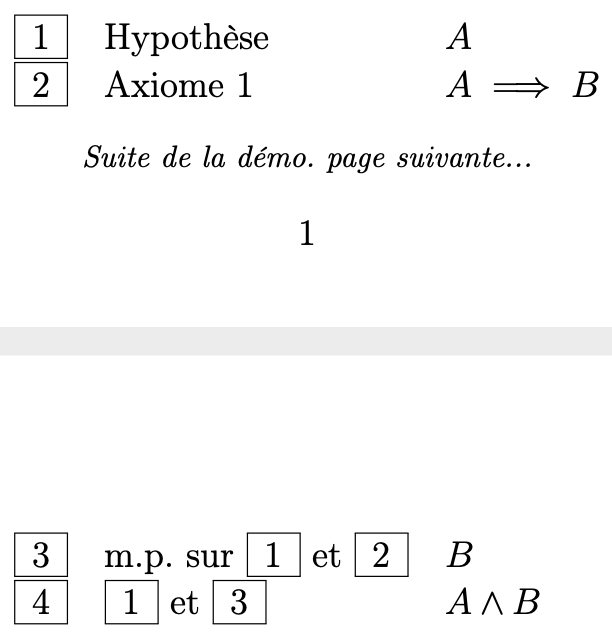
\includegraphics[scale = .5]{demo-explained-univ-broken[fr].png}}
\end{center}
%\section{Logique et fondements}

%\subsection{Détailler un \og vrai \fg{} raisonnement}

\subsubsection{Un tableau pour le collège et le lycée} \label{explain-hard-proof-for-youngs}


\newparaexample{Avec les réglages par défaut}

L'environnement étoilé \env{demoexplain*} est différent de l'environnement \env{demoexplain} puisqu'il sert à indiquer trois choses et non juste deux comme le montre l'exemple suivant
\footnote{
	C'est pour cela qu'est proposé une version étoilée de l'environnement et non l'utilisation d'une option de l'environnement non étoilé. 
}.
Par contre, la syntaxe est très similaire.
Notez au passage la possibilité d'utiliser \macro{newline} pour forcer un retour à la ligne dans une cellule.

\begin{latexex-flat}
\begin{demoexplain*}
    \demostep
        $ABC$ est un triangle
        \newline équilatéral 
      & Dans un triangle équilatéral, les trois angles mesurent $60$\textdegree. 
      & $\anglein{ABC} = 60$\textdegree     
    \demostep
        Voir la conséquence \explref*{1} .
      & Simple calcul avec conversion en radians.
      & $\dfrac{1}{3} \anglein{ABC} = \dfrac{\pi}{9}$
\end{demoexplain*}
\end{latexex-flat}


% ---------------------- %


\newparaexample{Avec toutes les options}

Le système de référence marche ici aussi.
Par contre \env{demoexplain*} ne propose que \verb+start+ comme clé optionnelle avec le même fonctionnement que pour \env{demoexplain}.

\begin{latexex-flat}
\begin{demoexplain*}[start = last]
    \demostep[demo-first-geo-fact]
        $ABC$ est un triangle \newline équilatéral 
      & Dans un triangle équilatéral, les trois angles mesurent $60$\textdegree. 
      & $\anglein{ABC} = 60$\textdegree     
    \demostep
        Voir la conséquence \explref{demo-first-geo-fact} .
      & Simple calcul avec conversion en radians.
      & $\dfrac{1}{3} \anglein{ABC} = \dfrac{\pi}{9}$
\end{demoexplain*}
\end{latexex-flat}


% ---------------------- %


\subsubsection{Un tableau sur plusieurs pages}

Un tableau devant utiliser plusieurs pages sera scindé comme ci-dessous sans perte d'information
\footnote{
	Tout le travail est fait par l'environnement \env{longtable} du package éponyme.
}.

\begin{center}
	\frame{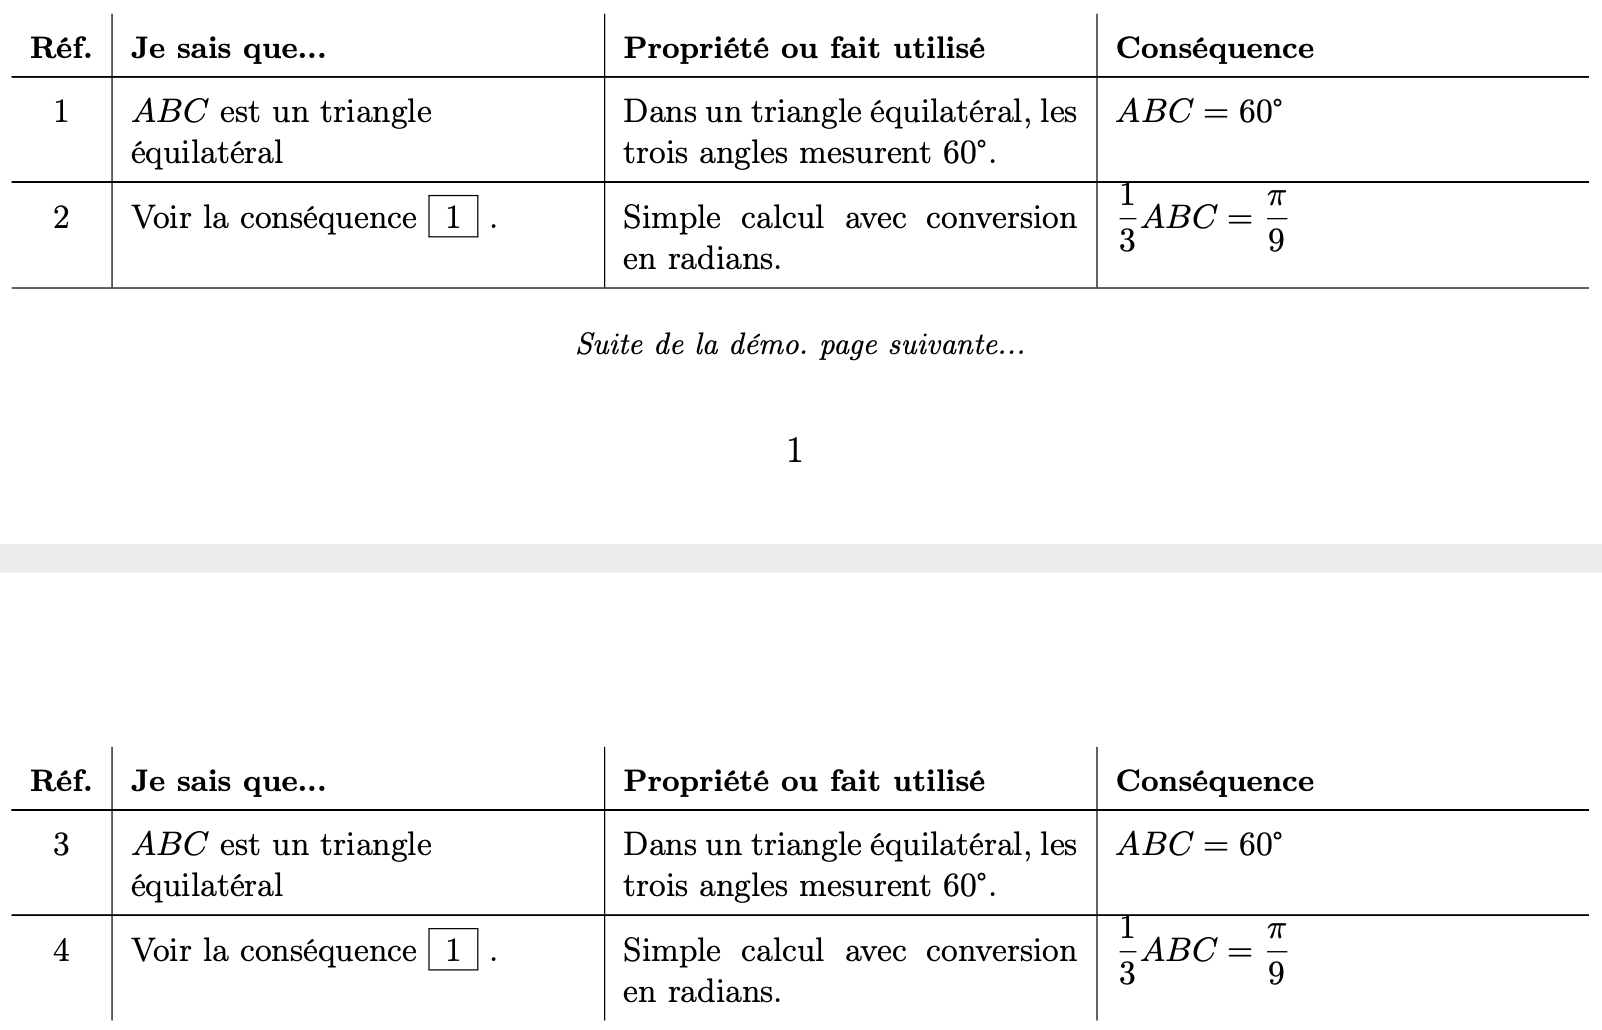
\includegraphics[scale = .5]{demo-explained-middleschool-broken[fr].png}}
\end{center}
%\section{Logique et fondements}

%\subsection{Détailler un raisonnement}
\section{Ensembles et applications}

\subsection{Différents types d'ensembles}

\subsubsection{Ensembles versus accolades}

\newparaexample{}

\begin{latexex}
$\setgene{1 ; 3 ; 5}$ .
\end{latexex}


% ---------------------- %


\newparaexample{}

Dans l'exemple suivant on utilise l'option \prefix{sb} pour \whyprefix{s}{mall} \whyprefix{b}{races} soit \inenglish{petites accolades}.

\begin{latexex}
$\setgene {\dfrac{1}{3} ; \dfrac{5}{7} ; 
           \dfrac{9}{11}}$

$\setgene*{\dfrac{1}{3} ; \dfrac{5}{7} ;
           \dfrac{9}{11}}$
\end{latexex}


% ---------------------- %


\subsubsection{Ensembles pour la géométrie} \label{set-geo}

\newparaexample{}

\begin{latexex}
$\setgeo{C}$ ,
$\setgeo{D}$ ou
$\setgeo{d}$
\end{latexex}

\begin{remark}
	Pour le moment, il n'est pas possible de taper \verb+$\setgeo{ABC}$+ avec plusieurs lettres.
\end{remark}


% ---------------------- %


\newparaexample{Avec des indices}

\begin{latexex}
$\setgeo*{C}{1}$ ou
$\setgeo*{C}{2}$
\end{latexex}


% ---------------------- %


\subsubsection{Ensembles probabilistes}

\newparaexample{}

\begin{latexex}
$\setproba{E}$ ou
$\setproba{G}$
\end{latexex}

\begin{remark}
	Pour le moment, il n'est pas possible de taper \verb+$\setproba{ABC}$+ avec plusieurs lettres.
\end{remark}


% ---------------------- %


\newparaexample{Avec des indices}

\begin{latexex}
$\setproba*{E}{1}$ ou
$\setproba*{E}{2}$
\end{latexex}


% ---------------------- %


\subsubsection{Ensembles pour l'algèbre générale}

\newparaexample{}

\begin{latexex}
$\setalge{A}$ ,
$\setalge{K}$ ,
$\setalge{h}$ ou
$\setalge{k}$
\end{latexex}

\begin{remark}
	Pour le moment, il n'est pas possible de taper \verb+$\setalge{ABC}$+ avec plusieurs lettres.
\end{remark}


% ---------------------- %


\newparaexample{Avec des indices}

\begin{latexex}
$\setalge*{k}{1}$ ou $\setalge*{k}{2}$
\end{latexex}


% ---------------------- %


\subsection{Ensembles classiques en mathématiques et en informatique théorique} 

\subsubsection{La liste complète}

Dans l'exemple suivant,
$\PP$ désigne l'ensemble des nombres premiers,
$\HH$ celui des quaternions,
$\OO$ celui des octonions et
$\FF$ un ensemble de nombres flottants \emph{(notation à préciser suivant le contexte)}.

\begin{latexex}
$\nullset$

$\NN$ , $\ZZ$ , $\PP$

$\DD$ , $\QQ$ , $\RR$ , $\CC$

$\HH$ , $\OO$

$\FF$
\end{latexex}


% ---------------------- %


\subsubsection{Ensembles classiques suffixés}

L'ensemble $\RR$ nous permet de voir tous les cas possibles. 

\begin{latexex}
$\RRn$ , $\RRp$ , $\RRs$ 

$\RRsn$ , $\RRsp$
\end{latexex}


Nous avons utilisé les suffixes \prefix{n} pour \whyprefix{n}{égatif}, \prefix{p} pour \whyprefix{p}{ositif} et \prefix{s} pour \whyprefix{s}{tar} soit \inenglish{étoile}. Il y a aussi les suffixes composites \prefix{sn} et \prefix{sp}.

\medskip

Notez qu'il est interdit d'utiliser \verb+$\CCn$+ pour $\setspecial{\CC}{n}$ car l'ensemble $\CC$ ne possède pas de structure ordonnée standard. Jetez un oeil à la section suivante pour apprendre à taper $\setspecial{\CC}{n}$ si vous en avez besoin. L'interdiction est ici purement sémantique !

\medskip

\begin{remark}
	La table \ref{table:suffixes-sets} \vpageref{table:suffixes-sets} montre les associations autorisées entre ensembles classiques et suffixes.
\end{remark}

% == Table of suffixes - START == %

\begin{table}[h]
    \caption{Suffixes}
    \begin{center}
        \begin{tabular}{c|c|c|c|c|c}
              & \verb+n+ & \verb+p+ & \verb+s+ & \verb+sn+ & \verb+sp+ \\
            \hline \makecell{\macro{NN}} &          &          & $\times$ &          &          \\
            \hline \makecell{\macro{PP}} &          &          &          &          &          \\
            \hline \makecell{\macro{ZZ}\\\macro{DD}\\\macro{QQ}\\\macro{RR}} & $\times$ & $\times$ & $\times$ & $\times$ & $\times$ \\
            \hline \makecell{\macro{CC}\\\macro{HH}\\\macro{OO}} &          &          & $\times$ &          &          \\
            \hline \makecell{\macro{FF}} & $\times$ & $\times$ & $\times$ & $\times$ & $\times$ \\
        \end{tabular}
    \end{center}
    \label{table:suffixes-sets}
\end{table}

% == Table of suffixes - END == %


% ---------------------- %


\subsection{Des suffixes à la carte}

\paragraph{Exemple d'utilisation}

Dans cet exemple, il faut savoir que le 2\ieme{} argument ne peut prendre que les valeurs \prefix{n}, \prefix{p}, \prefix{s}, \prefix{sn} ou \prefix{sp}.

\begin{latexex}
$\setspecial{\CC}{n}$ ,
$\setspecial{\HH}{sp}$ ou
$\setspecial*{\setproba{P}}{n}$
\end{latexex}


% ---------------------- %
% \section{Sets}

\subsection{Intervalles}

\subsubsection{Intervalles réels - Notation française (?\,)}

\newparaexample{}

Dans cet exemple, la syntaxe fait référence à 
\whyprefix{O}{pened} et \whyprefix{C}{losed}
pour
\inenglish{ouvert et fermé}.
Nous verrons que \prefix{CC} et \prefix{OO} sont contractés en \prefix{C} et \prefix{O}.
Notez au passage que la macro utilisée résout un problème d'espacement vis à vis du signe $=$ .

\begin{latexex}
$I = ]a ; b] = \intervalOC{a}{b}$
\end{latexex}


% ---------------------- %


\newparaexample{}

Les crochets s'étendent verticalement automatiquement. Pour empêcher cela, il suffit d'utiliser la version étoilée de la macro.
Dans ce cas, les crochets restent tout de même un peu plus grands que des crochets utilisés directement. Voici un exemple.

\begin{latexex}
$\displaystyle
 \intervalC{ \frac{1}{2} }{ 1^{2^{3}} }
 =
 [ \frac{1}{2} ; 1^{2^{3}} ]
 =
 \intervalC*{ \frac{1}{2} }{ 1^{2^{3}} }$
\end{latexex}


% ---------------------- %


\subsubsection{Intervalles réels - Notation américaine}

\newparaexample*{}

Dans cet exemple, la syntaxe fait référence à \whyprefix{P}{arenthèse}. Cette notation est utilisée États Unis.

\begin{latexex}
$\intervalPC{a}{b} = \intervalOC{a}{b}$
et
$\intervalP{a}{b} = \intervalO{a}{b}$.
\end{latexex}


% ---------------------- %


\subsubsection{Intervalles discrets d'entiers}

\newparaexample*{}

Dans l'exemple, la syntaxe fait référence à $\ZZ$ l'ensemble des entiers relatifs.

\begin{latexex}
 $\ZintervalC{-1}{4} 
  \eqdef
  \{ -1 ; 0 ; 1 ; 2 ; 3 ; 4 \}$
 
 $\ZintervalC{-1}{4} 
= \ZintervalO{-2}{5}$.
\end{latexex}


% ---------------------- %
% \section{Sets}

\subsection{Unions et intersections}

\newparaexample{Des unions}

Ci-dessous est utilisée la macro \macro{bigcup} proposée par le package \verb+amssymb+.

\begin{latexex}
$A \cup B$

$\dcup_{k=1}^{n} A_k$

$\bigcup_{k=1}^{n} B_k$

$\displaystyle \bigcup_{k=1}^{n} C_k$
\end{latexex}


% ---------------------- %


\newparaexample{Des unions disjointes}

Ci-dessous sont utilisées les macros \macro{sqcup} et \macro{bigsqcup} proposée par le package \verb+amssymb+.

\begin{latexex}
$A\sqcup B$

$\dsqcup_{k=1}^{n} A_k$

$\bigsqcup_{k=1}^{n} B_k$

$\displaystyle \bigsqcup_{k=1}^{n} C_k$
\end{latexex}


% ---------------------- %


\newparaexample{Des intersections}

Ci-dessous est utilisée la macro \macro{bigcap} proposée par le package \verb+amssymb+.

\begin{latexex}
$A \cap B$

$\dcap_{k=1}^{n} A_k$

$\bigcap_{k=1}^{n} B_k$

$\displaystyle \bigcap_{k=1}^{n} C_k$
\end{latexex}


% ---------------------- %
% \section{Sets}

\subsection{Cardinal, image et compagnie}

\newparaexample{Cardinal}

\begin{latexex}
$\card* E = \card E$
\end{latexex}


% ---------------------- %


\newparaexample{Image et compagnie}

\begin{latexex}
$\ker f$ , $\dom f$ ,
$\im f$ ou $\codom f$
\end{latexex}


% ---------------------- %
%\section{Logique et fondements}

\subsection{Application totale, partielle, injective, surjective et/ou bijective} \label{section:application}

Voici des symboles qui, bien que très techniques, facilitent la rédaction de documents à propos des applications totales ou partielles
\footnote{
	$a: E \to F$ est une application totale si $\forall x \in E$, $\existsone y \in F$ tel que $y = a(x)$. 
	Plus généralement, $f: E \to F$ est une application partielle si $\forall x \in E$, $\existmulti{\leq 1} y \in F$ tel que $y = f(x)$, autrement dit soit $f(x)$ existe dans $F$, soit $f$ n'est pas définie en $x$.
}
\emph{(on parle aussi d'applications, sans qualificatif, et de fonctions)}.


% ---------------------- %


\newparaexample{Applications totales}

\begin{latexex-flat}
$f: A \to B$ est une application totale, c'est à dire définie sur $A$ tout entier.

$i: C \onetoone D$ est une application totale injective.

$s: E \onto F$ est une application totale surjective.

$b: G \biject H$ est une application totale bijective.
\end{latexex-flat}


% ---------------------- %


\newparaexample{Applications partielles}

\begin{latexex-flat}
$f: A \pto B$ est une application partielle, c'est à dire définie sur
un sous-ensemble de $A$.

$i: C \ponetoone D$ est une application partielle injective.

$s: E \ponto F$ est une application partielle surjective.

$b: G \pbiject H$ est une application partielle bijective.
\end{latexex-flat}


% ---------------------- %
\section{Géométrie}

\subsection{Points et lignes}

\subsubsection{Points}

\newparaexample{Sans indice}

\begin{latexex}
$\pt{I}$
\end{latexex}


% ---------------------- %


\newparaexample{Avec un indice}

\begin{latexex}
$\pt*{I}{1}$ ou
$\pt*{I}{2}$
\end{latexex}


% ---------------------- %


\subsubsection{Lignes}

\newparaexample{Les droites}

Dans l'exemple suivant, le préfixe \prefix{g} est pour \whyprefix{g}{éometrie} tandis que \prefix{p} est pour \whyprefix{p}{oint}.

\begin{latexex}
$\gline{A}{B}$ ,
$\gline{\pt{A}}{\pt{B}}$ ou
$\pgline{A}{B}$
\end{latexex}


% ---------------------- %


\newparaexample{Les segments}

Les macros \macro{segment} et \macro{psegment} ont un comportement similaire à \macro{gline} et \macro{pgline}.

\begin{latexex}
$\segment{A}{B}$ ,
$\segment{\pt{A}}{\pt{B}}$ ou
$\psegment{A}{B}$
\end{latexex}


% ---------------------- %


\newparaexample{Les demi-droites}

Dans l'exemple suivant, le préfixe \prefix{h} est pour \whyprefix{h}{alf}  soit \inenglish{moitié}.

\begin{latexex}
$\hgline{A}{B}$ ,
$\hgline{\pt{A}}{\pt{B}}$ ou
$\phgline{A}{B}$
\end{latexex}


% ---------------------- %


\newparaexample{D'autres demi-droites}

Ce qui suit nécessite d'utilise l'argument optionnel de \macro{gline} et \macro{pgline}. La valeur \prefix{OC} provient de \whyprefix{O}{pened} -- \whyprefix{C}{losed} soit \inenglish{ouvert -- fermé}.

\begin{latexex}
$\gline[OC]{A}{B}$ ,
$\gline[OC]{\pt{A}}{\pt{B}}$ ou
$\pgline[OC]{A}{B}$
\end{latexex}


\begin{remark}
	Les segments utilisent en fait l'option \prefix{C} et les demi-droites standard l'option \prefix{CO}.
	La valeur par défaut est \prefix{O}.
\end{remark}


% ---------------------- %


\subsubsection{Droites parallèles ou non}

Les opérateurs \macro{parallel} et \macro{nparallel} utilisent des obliques au lieu de barres verticales comme le montre l'exemple qui suit où \macro{stdnparallel} est un alias de \macro{nparallel} fourni par le package \verb+amssymb+, et \macro{stdparallel} est un alias de la version standard de \macro{parallel} proposée par \LaTeX{}.

\begin{latexex}
$\pgline{A}{B} \parallel \pgline{C}{D}$
au lieu de
$\pgline{A}{B}
 \stdparallel \pgline{C}{D}$

$\pgline{E}{F} \nparallel \pgline{G}{H}$
au lieu de
$\pgline{E}{F}
 \stdnparallel \pgline{G}{H}$
\end{latexex}


% ---------------------- %
% \section{Géométrie}

\subsection{Vecteurs}

\subsubsection{Les écrire}

\newparaexample{}

\begin{latexex}
$\vect{ABCDEF}$  ,
$\vect*{e}{rot}$ ou
$\vect{e_{rot}}$
\end{latexex}


% ---------------------- %


\newparaexample{}

\begin{latexex}
$\vect{i}$ ou
$\vect*{j}{2}$
\end{latexex}


% ---------------------- %
% \section{Géométrie}

%\subsection{Vecteurs}

\subsubsection{Norme}

Ci-dessous l'argument optionnel de \macro{vnorm} vaut \prefix{b} par défaut pour \whyprefix{b}{ig} soit \inenglish{gros} mais l'on peut aussi utiliser \prefix{s} pour \whyprefix{s}{mall} soit \inenglish*{petit}. Par contre \macro{vnorm} n'a pas d'option.

\begin{latexex}
 $\norm{\vect{i}} = \vnorm{i}$

 $\norm   {\dfrac{2}{7} \vect*{e}{k}}
= \norm[s]{\dfrac{2}{7} \vect*{e}{k}}$
\end{latexex}


\begin{remark}
	Le code \LaTeX{} pour des doubles barres extensibles ou non vient directement de ce message : \url{https://tex.stackexchange.com/a/43009/6880}.
\end{remark}


% ---------------------- %
% \section{Géométrie}

%\subsection{Vecteurs}

\subsubsection{Produit scalaire}

\newparaexample{Version longue}

\begin{latexex}
$\dotprod{\dfrac{1}{2} \vect{u}}%
         {\vect{v}}$
\end{latexex}


% ---------------------- %


\newparaexample{Écriture \og à la physicienne \fg}

Dans l'exemple suivant, l'option \prefix{r} est pour \whyprefix{r}{after} soit \inenglish{chevron}, et dans \prefix{sr} le \prefix{s} est pour \whyprefix{s}{mall} soit \inenglish{petit}. Les physiciens aiment bien cette notation.

\begin{latexex}
$\dotprod[r] {\dfrac{1}{2} \vect{u}}%
             {\vect{v}}$

$\dotprod[sr]{\dfrac{1}{2} \vect{u}}%
             {\vect{v}}$
\end{latexex}


% ---------------------- %


\newparaexample{Version courtes mais restrictive}

Dans l'exemple suivant, le préfixe \prefix{v} est pour \whyprefix{v}{ecteur}.

\begin{latexex}
$\vdotprod    {u}{v}$
 
$\vdotprod[r] {u}{v}$ comme
$\vdotprod[sr]{u}{v}$
\end{latexex}


% ---------------------- %

%
%\newparaexample{Écriture formelle développée}
%
%Ce qui suit peut rendre service... ou pas.
%Dans l'exemple ci-dessous \prefix{exp} est pour \whyprefix{exp}{and} c'est à dire \inenglish{développer}, \prefix{c} pour \macro{cdot} et enfin \prefix{t} pour \macro{times}.
%
%\begin{latexex}
%$\dotprod[exp]{\vect{u}}{\vect{v}}$
%
%$\vdotprod[cexp]{u}{v}$
%
%$\vdotprod[texp]{u}{v}$
%\end{latexex}


% ---------------------- %
% \section{Géométrie}

%\subsection{Vecteurs}

\subsubsection{Produit vectoriel}

\paragraph{Exemple 1 - Écriture symbolique - Version longue}

\begin{latexex}
$\crossprod{\dfrac{1}{2} \vect{i}}%
           {\vect{j}}$ 
\end{latexex}


% ---------------------- %


\paragraph{Exemple 2 - Écriture symbolique - Version courte mais restrictive}

\begin{latexex}
$\vcrossprod{i}{j}$
\end{latexex}


% ---------------------- %


\paragraph{Exemple 3 - Explication des calculs}

Dans l'exemple suivant, le préfixe \prefix{calc} est pour \whyprefix{calc}{uler} et \prefix{v} pour \whyprefix{v}{ecteur}.

\begin{latexex}
$\calccrossprod {\vect{u}}{x }{y }{z }%
                {\vect{v}}{x'}{y'}{z'}
 =
 \vcalccrossprod{u       }{x }{y }{z }%
                {v       }{x'}{y'}{z'}$

$\vcalccrossprod{AB}{x_B - x_A}%
                    {y_B - y_A}%
                    {z_B - z_A}%
                {CD}{x_D - x_C}%
                    {y_D - y_C}%
                    {z_D - z_C}$
\end{latexex}


Avec un public averti on peut juste proposer les coordonnées sans les décorations comme ci-après via la version étoilée de \macro{vcalccrossprod} mais ceci fonctionne aussi avec \macro{calccrossprod}.

\begin{latexex}
$\vcalccrossprod*{u}{x }{y }{z }%
                 {v}{x'}{y'}{z'}$
\end{latexex}


Enfin si les vecteurs vous gênent il suffira d'utiliser l'option \verb+novec+ pour \verb+no+ \whyprefix{vec}{tor} soit \inenglish{pas de vecteur} comme ci-après.
Ceci fonctionne aussi pour la macro \macro{calccrossprod}.
Il peut sembler un peu lourd d'avoir des arguments pour des vecteurs non affichés mais ce choix permet à l'usage de faire des copier-coller redoutables d'efficacité !

\begin{latexex}
$\vcalccrossprod[novec]{u}{x }{y }{z }%
                       {v}{x'}{y'}{z'}
 =
 \vcalccrossprod*[novec]{u}{x }{y }{z }%
                        {v}{x'}{y'}{z'}$
\end{latexex}


% ---------------------- %


\paragraph{Exemple 4 - Les coordonnées  \og détaillées \fg}

Pour avoir le détail directement dans des coordonnées vous pouvez faire appel à la macro \macro{coordcrossprod} où le préfixe \prefix{coord} fait référence à \whyprefix{coord}{onnée}
\footnote{
	En coulisse on utilise la macro \macro{coord} présentée dans la section \ref{coordinates} page \pageref{coordinates}. 
}.
On peut utiliser des options pour choisir certains paramètres de mise en forme.

\begin{latexex}
$\coordcrossprod{\dfrac{1}{2}x}{y }{z }%
                {x'           }{y'}{z'}$

$\coordcrossprod[vb]%
                {\dfrac{1}{2}x}{y }{z }%
                {x'           }{y'}{z'}$

$\coordcrossprod[sp,c]%
                {\dfrac{1}{2}x}{y }{z }%
                {x'           }{y'}{z'}$
\end{latexex}


Voici les options disponibles. Nous expliquons ensuite comment les utiliser.
\begin{enumerate}
	\item \prefix{p} vient de \whyprefix{p}{arenthèses}. Ceci donnera une écriture horizontale.

	\item \prefix{b} vient de \whyprefix{b}{rackets} soit \inenglish{crochets}. Ceci donnera une écriture horizontale.

	\item \prefix{sp} et \prefix{sb} produisent des délimiteurs non extensibles en mode horizontal.
	      Ici \prefix{s} vient de \whyprefix{s}{mall} soit \inenglish{petit}.

	\item \prefix{vp} et \prefix{vb} produisent des écritures verticales.
	      Ici \prefix{v} vient de \whyprefix{v}{ertical}.

	\medskip

	\item \prefix{s} tout seul demande d'utiliser un espace pour séparer les facteurs de chaque produit.

	\item \prefix{t} tout seul demande d'utiliser \macro{times} comme opérateur de multiplication.

	\item \prefix{c} tout seul demande d'utiliser \macro{cdot} comme opérateur de multiplication.
\end{enumerate}


On peut indiquer des options vis à vis du mode vertical ou horizontal avec des délimiteurs extensibles ou non éventuellement, ou bien sur le symbole pour les produits. On peut aussi combiner deux de ces typs de choix en les séparant par une virgule ce qui fait un total de $6\times3 = 18$ combinaisons possibles.
La valeur par défaut est \verb+p,s+.


\bigskip


\textbf{Attention !}
Les produits sont produits stupidement. Autrement dit ce sera à vous d'ajouter des parenthèses là où il y en aura besoin sinon vous obtiendrez des horreurs comme celle ci-dessous.
    
\begin{latexex}
$\coordcrossprod[vb]{x_B - x_A}%
                    {y_B - y_A}%
                    {z_B - z_A}%
                    {x_D - x_C}%
                    {y_D - y_C}%
                    {z_D - z_C}$
\end{latexex}

Ici nous n'avons pas d'autre choix que de corriger le tir nous-même.
Ceci étant indiqué, ce genre de situation est très rare dans la vraie vie mathématique où l'on évite d'avoir à calculer un produit vectoriel avec des expressions compliquées.
    
\begin{latexex}
$\coordcrossprod[vb]{(x_B - x_A)}%
                    {(y_B - y_A)}%
                    {(z_B - z_A)}%
                    {(x_D - x_C)}%
                    {(y_D - y_C)}%
                    {(z_D - z_C)}$
\end{latexex}


% ---------------------- %
% \section{Géométrie}

%\subsection{Vecteurs}

\subsubsection{Plan -- Déterminant de deux vecteurs} \label{colinearity-criteria}

\newparaexample{Version décorée}

Dans l'exemple suivant, le préfixe \prefix{calc} est pour \whyprefix{calc}{uler}.

\begin{latexex}
$\calcdetplane{\vect{u}}{x }{y }%
              {\vect{v}}{x'}{y'}$
ou
$\calcdetplane{\vect{AB}}%
              {x_B - x_A}{y_B - y_A}%
              {\vect{CD}}%
              {x_D - x_C}{y_D - y_C}$
\end{latexex}


% ---------------------- %


\newparaexample{Version non décorée}

\begin{latexex}
$\calcdetplane*{\vect{u}}{x }{y }%
               {\vect{v}}{x'}{y'}$
\end{latexex}


% ---------------------- %


\newparaexample{Rédaction raccourcie pour les vecteurs}

Dans l'exemple suivant, le préfixe \prefix{v} est pour \whyprefix{v}{ecteur}.

\begin{latexex}
$\vcalcdetplane{u}{x }{y }%
               {v}{x'}{y'}
 =
 \vcalcdetplane*{u}{x }{y }%
                {v}{x'}{y'}$
\end{latexex}


% ---------------------- %


\newparaexample{Versions sans les vecteurs}

Dans l'exemple suivant, on utilise la valeur \verb+novec+ pour l'argument optionnel de \macro{vcalcdetplane} qui par défaut est \verb+vec+ pour pour \whyprefix{vec}{teur}.
À l'usage ceci permet des copier-coller très efficaces !


\begin{latexex}
 $\vcalcdetplane[novec] {u}{x }{y }%
                        {v}{x'}{y'}
= \vcalcdetplane*[novec]{u}{x }{y }%
                        {v}{x'}{y'}$
\end{latexex}


\begin{remark}
	Ce qui précède marche aussi avec les macros \macro{calcdetplane} et \macro{calcdetplane*}.
\end{remark}


% ---------------------- %


\newparaexample{Calcul développé}

Grâce à l'argument optionnel de \macro{calcdetplane} ou \macro{vcalcdetplane}, il est aussi possible d'obtenir le résultat développé du calcul comme ci-après
où \prefix{exp} est pour \whyprefix{exp}{and} soit \inenglish{développer}, \prefix{c} pour \macro{cdot} et enfin \prefix{t} pour \macro{times}.
Même si les vecteurs ne sont pas utilisés pour la mise en forme, on obtient ici une méthode très pratique à l'usage car permettant de faire des copier-coller.

\begin{latexex}
$\vcalcdetplane[exp]{u}{x }{y }%
                    {v}{x'}{y'}$

$\vcalcdetplane[cexp]{u}{x }{y }%
                     {v}{x'}{y'}$

$\vcalcdetplane[texp]{u}{x }{y }%
                     {v}{x'}{y'}$
\end{latexex}


\begin{remark}
	Ce qui précède marche aussi avec les versions étoilées.
\end{remark}


\textbf{Attention !}
Le développement effectué est stupide. Autrement dit ce sera à vous d'ajouter des parenthèses là où il y en aura besoin sinon vous obtiendrez des horreurs comme celle qui suit.
    
\begin{latexex}
$\vcalcdetplane[exp]{AB}%
                    {x_B - x_A}%
                    {y_B - y_A}%
                    {CD}%
                    {x_D - x_C}%
                    {y_D - y_C}$
\end{latexex}

Ici nous n'avons pas d'autre choix que de régler le problème à la amin. Ce genre de situation n'est pas rare dans la vraie vie mathématique.
    
\begin{latexex}
$\vcalcdetplane[exp]{AB}%
                    {(x_B - x_A)}%
                    {(y_B - y_A)}%
                    {CD}%
                    {(x_D - x_C)}%
                    {(y_D - y_C)}$
\end{latexex}


% ---------------------- %
%\section{Géométrie}

\subsection{Coordonnées} \label{coordinates}

\newparaexample{Des coordonnées seules}

\verb+lymath+ propose, via un argument optionnel, six façons différentes de rédiger des coordonnées seules \emph{(nous verrons après des macros pour les coordonnées d'un point et celles d'un vecteur afin de produire un code \LaTeX{} plus sémantique)}. Commençons par les écritures horizontales où vous noterez l'utilisation de \verb+|+ pour séparer les coordonnées dont le nombre peut être quelconque.

\begin{latexex}
$\coord    {\dfrac{1}{3} | -4 | 0}$ ou
$\coord[sp]{\dfrac{1}{3} | -4 | 0}$

$\coord[b] {\dfrac{1}{3} | -4 | 0}$ ou
$\coord[sb]{\dfrac{1}{3} | -4 | 0}$
\end{latexex}


Il existe en plus deux versions verticales.

\begin{latexex}
$\coord[vp]{3 | -4}$ ou
$\coord[vb]{3 | -4}$
\end{latexex}


Voici d'où viennent les noms des options.
\begin{enumerate}
	\item \prefix{p}, qui est aussi la valeur par défaut, vient de \whyprefix{p}{arenthèses}.

	\item \prefix{b} vient de \whyprefix{b}{rackets} soit \inenglish{crochets}.

	\item \prefix{s} pour \whyprefix{s}{mall} soit \inenglish{petit} permet d'avoir des délimiteurs non extensibles en mode horizontal car par défaut ils le sont.

	\item \prefix{v} pour \whyprefix{v}{ertical} demande de produire une écriture verticale.
\end{enumerate}


% ---------------------- %


\newparaexample{Coordonnées d'un point}

La macro \macro{pcoord} avec \prefix{p} pour  \whyprefix{p}{oint} prend un argument supplémentaire avant les coordonnées qui est le nom d'un point qui sera mis en forme par la macro \macro{pt}. Si vous ne souhaitez pas que \macro{pt} soit appliquée, il suffit de passer via la version étoilée \macro{pcoord*}.

\begin{latexex}
$\pcoord{A}{3 | -4 | 0 | -1}$ ou
$\pcoord*{\Sigma}{7 | 9 | 8}$
\end{latexex}


Toutes les options disponibles avec \macro{coord} le sont aussi avec  \macro{pcoord}. 

\begin{latexex}
$\pcoord[b]{A}{3 | -4 | 0 | -1}$ ou
$\pcoord*[b]{\Sigma}{7 | 9 | 8}$
\end{latexex}



% ---------------------- %


\newparaexample{Coordonnées d'un vecteur}

Le fonctionnement de \macro{vcoord} est similaire à celui de \macro{pcoord} si ce n'est que c'est la macro \macro{vect} qui sera appliquée si besoin.

\begin{latexex}
$\vcoord{u}{3 | -4}$ ou
$\vcoord*{\dfrac{1}{2} \vect{u}}%
         {3 | -4}$

$\vcoord[vp]{u}{3 | -4}$ ou
$\vcoord*[vp]{\dfrac{1}{2} \vect{u}}%
             {3 | -4}$
\end{latexex}


% ---------------------- %
% \section{Géométrie}

\subsection{Nommer un repère}

\newparaexample{La méthode basique}

Commençons par la manière la plus basique d'écrire un repère \textit{(nous verrons d'autres méthodes qui peuvent être plus efficaces)}.

\begin{latexex}
$\axes{\pt{O} %
     | \pt{I} | \pt{J}}$
\end{latexex}


% ---------------------- %


\newparaexample{La méthode basique en version étoilée}

Dans l'exemple ci-dessous, on voit que la version étoilée produit des petites parenthèses.
\begin{latexex}
$\axes{\pt{O} %
     | \dfrac{7}{3} \vect{i} %
     | \vect{j}}$
ou
$\axes*{\pt{O} %
     | \dfrac{7}{3} \vect{i} %
     | \vect{j}}$
\end{latexex}


% ---------------------- %


\newparaexample{La méthode basique en dimension quelconque}

Il faut au minimum deux "morceaux" séparés par des barres \verb+|+, cas de la dimension $1$, mais il n'y a pas de maximum, cas d'une dimension quelconque $n > 0$.

\begin{latexex}
$\axes{\pt{O} %
     | \vect*{i}{1} %
     | \vect*{i}{2} %
     | \vect*{i}{3} %
     | \dots %
     | \vect*{i}{9} %
     | \vect*{i}{10} %
     | \vect*{i}{11} %
     | \vect*{i}{12}}$
\end{latexex}


% ---------------------- %


\newparaexample{Repère affine}

Dans l'exemple suivant, le préfixe \prefix{p} est pour \whyprefix{p}{oint}.

\begin{latexex}
$\paxes{O | I | J | K}$
au lieu de
$\axes{\pt{O} %
     | \pt{I} | \pt{J} | \pt{K}}$
\end{latexex}


% ---------------------- %


\newparaexample{Repère vectoriel (méthode 1)}

Dans l'exemple suivant, le préfixe \prefix{v} est pour \whyprefix{v}{ecteur}.

\begin{latexex}
$\vaxes{\pt{O} | i | j}$
au lieu de
$\axes{\pt{O} | \vect{i} | \vect{j}}$
\end{latexex}


% ---------------------- %


\newparaexample{Repère vectoriel (méthode 2)}

Dans l'exemple suivant, le préfixe \prefix{pv} permet de combiner ensemble les fonctionnalités proposées par les préfixes \prefix{p} et \prefix{v}.

\begin{latexex}
$\pvaxes{O | i | j}$
au lieu de
$\axes{\pt{O} | \vect{i} | \vect{j}}$
\end{latexex}


% ---------------------- %
% \section{Géométrie}

\subsection{Arcs circulaires}

\newparaexample{}

\begin{latexex}
$\circarc{ABCDEF}$ ,
$\circarc*{A}{rot}$ ou
$\circarc{A_{rot}}$
\end{latexex}


% ---------------------- %


\newparaexample{}

\begin{latexex}
$\circarc{i}$ ou
$\circarc*{j}{2}$
\end{latexex}


% ---------------------- %
% \section{Géométrie}

\subsection{Angles}

\subsubsection{Angles géométriques \og intérieurs \fg}

\newparaexample{}

\begin{latexex}
$\anglein {ABCDEF}$

$\anglein* {A}{rot}$

$\anglein {A_{rot}}$
\end{latexex}


% ---------------------- %


\newparaexample{Cacher les points du i et du j}

\begin{latexex}
$\anglein{i}$ et
$\anglein*{j}{2}$
\end{latexex}


% ---------------------- %
% \section{Géométrie}

%\subsection{Angles}

\subsubsection{Angles orientés de vecteurs}

\paragraph{Sans chapeau - Version longue}

L'option par défaut est \prefix{p} pour \whyprefix{p}{arenthèse}.
Dans \prefix{sp} le \prefix{s} est pour \whyprefix{s}{mall} soit \inenglish{petit}.
 
\begin{latexex}
$\angleorient    {\dfrac{1}{2} \vect{i}}%
                 {\vect{j}}$

$\angleorient[sp]{\dfrac{1}{2} \vect{i}}%
                 {\vect{j}}$
\end{latexex}


% ---------------------- %


\paragraph{Sans chapeau - Version courte mais restrictive}

Dans l'exemple suivant, le préfixe \prefix{v} est pour \whyprefix{v}{ecteur} qui permet de simplifier la saisie quand l'on a juste des vecteurs nommés avec des lettres
\emph{(notez que l'option \prefix{sp} n'apporte rien de nouveau)}.

\begin{latexex}
$\vangleorient    {i}{j}$ comme
$\vangleorient[sp]{i}{j}$
\end{latexex}


% ---------------------- %


\paragraph{Avec un chapeau}

Dans l'exemple suivant, \prefix{h} est pour \whyprefix{h}{at} soit \inenglish{chapeau}.
Notez au passage que \prefix{sh} produit juste des parenthèses petites mais ce choix de nom simplifie l'utilisation de la macro \emph{(c'est mieux que \prefix{hsp} par exemple)}.

\begin{latexex}
$\angleorient[h] {\dfrac{1}{2} \vect{i}}%
                 {\vect{j}}$

$\angleorient[sh]{\dfrac{1}{2} \vect{i}}%
                 {\vect{j}}$

$\vangleorient[h] {i}{j}$ comme
$\vangleorient[sh]{i}{j}$
\end{latexex}


% ---------------------- %
\section{Analyse}

\subsection{Constantes et paramètres}

\subsubsection{Constantes classiques}

\paragraph{La liste complète}

% List of classical constants - START

\begin{latexex}
$\ggamma$ , $\ppi$ , $\ttau$ ,
$\ee$ , $\ii$ , $\jj$ 
et $\kk$ où $\ttau = 2 \ppi$
\end{latexex}

% List of classical constants - END


\begin{remark}
	Faites attention car \verb+{\Large $\ppi \neq \pi$}+ produit {\Large $\ppi \neq \pi$}. Comme vous le constatez, les symboles ne sont pas identiques. Ceci est vraie pour toutes les constantes grecques.
\end{remark}


% ---------------------- %


\subsubsection{Constantes latines personnelles}

\newparaexample*{}

La macro \macro{param} est surtout là pour une utilisation pédagogique.

\begin{latexex}
$\param{a} x^2 + \param{b} x + \param{c}$
ou
$a x^2 + b x + c$
\end{latexex}


% ---------------------- %
% \section{Analysis}

\subsection{La fonction valeur absolue}

\newparaexample*{}

\begin{latexex}
$\abs{2}$ ,
$\abs {\dfrac{3}{5}}$ ou
$\abs*{\dfrac{3}{5}}$
\end{latexex}


\begin{remark}
	Le code \LaTeX{} vient directement de ce poste : \url{https://tex.stackexchange.com/a/43009/6880}.
\end{remark}


% ---------------------- %
% \section{Analysis}

\subsection{Fonctions nommées spéciales}

\subsubsection{Sans paramètre}

\newparaexample*{}

Quelques fonctions nommées supplémentaires où \prefix{fch} est pour \whyprefix{f}{rench} soit \inenglish{français} \emph{(ce choix a été fait pour éviter des incompatibilités avec quelques autres packages)}. La liste complète des fonctions nommées est donnée un peu plus bas dans une section dédiée.

\begin{latexex}
$\fch x \neq ch x$ ,
$\ppcm(x;y)$ ou
$\lg x$
\end{latexex}


% ---------------------- %


\subsubsection{Avec un paramètre}

\newparaexample*{}

\begin{latexex}
$\logb{2} x = \lg x$ ou
$\expb{6} y = 6^y$
\end{latexex}


% ---------------------- %


\subsubsection{Toutes les fonctions nommées en plus}

\vspace{-1em}

\begin{multicols}{2}
% Table of all - START
\verb+pgcd+ : $\pgcd\dots$

\verb+ppcm+ : $\ppcm\dots$

\verb+acos+ : $\acos\dots$

\verb+asin+ : $\asin\dots$

\verb+atan+ : $\atan\dots$

\verb+arccosh+ : $\arccosh\dots$

\verb+arcsinh+ : $\arcsinh\dots$

\verb+arctanh+ : $\arctanh\dots$

\verb+acosh+ : $\acosh\dots$

\verb+asinh+ : $\asinh\dots$

\verb+atanh+ : $\atanh\dots$

\verb+fch+ : $\fch\dots$

\verb+fsh+ : $\fsh\dots$

\verb+fth+ : $\fth\dots$

\verb+afch+ : $\afch\dots$

\verb+afsh+ : $\afsh\dots$

\verb+afth+ : $\afth\dots$

\verb+expb{p}+ : $\expb{p}\dots$

\verb+logb{p}+ : $\logb{p}\dots$
% Table of all - END
\end{multicols}
% \section{Analysis}

\subsection{Des notations complémentaires pour des suites spéciales}

\newparaexample*{}

\begin{latexex}
$\seqplus{F}{1}{2}$

$\seqhypergeo{F}{1}{2}$

$\seqsuprageo{F}{1}{2}{3}{4}$
pour les fous\dots :-)
\end{latexex}


% ---------------------- %
% \section{Analysis}

\subsection{Calcul différentiel}

\subsubsection{\texorpdfstring{Les opérateurs $\pp{}$ et $\dd{}$}%
                               {Les opérateurs "d rond" et "d droit"}}

\newparaexample{}

\begin{latexex}
$\dd{t} = \dd[1]{t}$ ou $\dd[n]{x}$

$\pp{t} = \pp[1]{t}$ ou $\pp[n]{x}$
\end{latexex}


% ---------------------- %


\subsubsection{Dérivations totales d'une fonction -- Version longue mais polymorphe}

\newparaexample{Différentes écritures possibles}

La macro \macro{der} est stricte du point de vue sémantique car on doit lui fournir la fonction, l'ordre de dérivation et la variable de dérivation
\emph{(voir la section \ref{short-der} qui présente la macro \macro{sder} permettant une rédaction efficace pour obtenir $\sder[e]{f}{1}$ ou $\sder{f}{1}$)}.
Voici plusieurs mises en forme faciles à taper via l'option de \macro{der}.
Attention bien entendu à n'utiliser l'option par défaut \prefix{u} qu'avec un ordre de dérivation de valeur naturelle connue !

\begin{latexex}
 $\der   {f}{3}{x}
= \der[e]{f}{3}{x}$

 $\der[i] {u}{k}{x}
= \der[f] {u}{k}{x}
= \der[sf]{u}{k}{x}$
\end{latexex}


On peut aussi ajouter autour de la fonction des parenthèses extensibles ou non.
Ci-dessous on montre aussi une écriture du type \emph{\og opérateur fonctionnel \fg}.

\begin{latexex}
 $\der[osf,sp]{\frac{1}{2} uv}{k}{x}
= \der[of,p]  {\dfrac{1}{2} uv}{k}{x}$
\end{latexex}


\begin{remark}
	Expliquons les valeurs des options.
	\begin{enumerate}
		\item \prefix{u}, la valeur par défaut, est pour \whyprefix{u}{suel} soit l'écriture avec les primes. Cette option ne marchera pas avec un nombre symbolique de dérivations. 

		\item \prefix{e} est pour \whyprefix{e}{xposant}.

		\item \prefix{i} est pour \whyprefix{i}{ndice}.

		\item \prefix{f} est pour \whyprefix{f}{raction} avec aussi \prefix{sf} pour une écriture réduite où \prefix{s} est pour \whyprefix{s}{mall} soit \inenglish{petit}.

		\item \prefix{of} et \prefix{osf} utilisent le préfixe \prefix{o} pour \whyprefix{o}{pérateur}.
		
		\smallskip
		\item \prefix{p} est pour \whyprefix{p}{arenthèse} : dans ce cas les parenthèses seront extensibles.

		\item \prefix{sp} est pour des parenthèses non extensibles.
	\end{enumerate}
\end{remark}


% ---------------------- %


\newparaexample{Pas de uns inutiles}

\begin{latexex}
 $\der[i ]{u}{1}{x}
= \der[f ]{u}{1}{x}
= \der[sf]{u}{1}{x}
= \der[of]{u}{1}{x}$
\end{latexex}


\begin{remark}
	Voici comment forcer les exposants $1$ si besoin.

	\begin{latexex}
 $\der[i ]{u}{\,\!1}{x}
= \der[f ]{u}{\,\!1}{x}
= \der[sf]{u}{\,\!1}{x}
= \der[of]{u}{\,\!1}{x}$
\end{latexex}
\end{remark}


% ---------------------- %


\subsubsection{Dérivations totales d'une fonction -- Version courte pour les écritures standard} \label{short-der}

Dans l'exemple suivant le code manque de sémantique car on n'indique pas la variable de dérivation.
Ceci étant dit à l'usage la macro \macro{sder} rend de grands services.
Ici le préfixe \prefix{s} est pour \whyprefix{s}{imple} voire \whyprefix{s}{impliste}...
Voici des exemples où de nouveau l'option par défaut \prefix{u} ne sera fonctionnelle qu'avec un ordre de dérivation de valeur naturelle connue !

\begin{latexex}
 $\sder{f}{1} = \der{f}{1}{x}$

 $\sder{f}{1}
= \sder[e]{f}{1}$

 $\sder[sp ]{\dfrac{1}{2} uv}{2}
= \sder[e,p]{\dfrac{1}{2} uv}{2}$
\end{latexex}


\begin{remark}
	Ici les seules options disponibles sont \prefix{u}, \prefix{e}, \prefix{p} et \prefix{sp}.
\end{remark}


% ---------------------- %


\subsubsection{L'opérateur de dérivation totale}

Ce qui suit peut rendre service au niveau universitaire.
Les options possibles sont \verb+f+, valeur par défaut, \verb+sf+ et \verb+i+ avec les mêmes significations que pour la macro \macro{der}.

\begin{latexex}
 $\derope    {k}{x}
= \derope[sf]{k}{x}
= \derope[i] {k}{x}$

 $\derope    {1}{x}
= \derope[sf]{1}{x}
= \derope[i] {1}{x}$
\end{latexex}


% ---------------------- %
% \section{Analysis}

%\subsection{Calcul différentiel}

\subsubsection{Dérivations partielles}

\newparaexample{Différentes écritures possibles}

La macro \macro{pder}
\footnote{
	\macro{partial} existe déjà pour obtenir $\partial$.
}
avec \prefix{p} pour \whyprefix{p}{artielle}
permet de rédiger des dérivées partielles en utilisant facilement plusieurs mises en forme via une option qui vaut \verb+f+ par défaut.
Cette macro attend une fonction, les dérivées partielles effectuées et l'ordre total de dérivation.
Voici les deux types de mise en forme où vous noterez comment \verb+x | y^2+ est interprété.

\begin{latexex}
 $\pder    {f}{x | y^2}{3}
= \pder[sf]{f}{x | y^2}{3}$
ou
 $\pder[i] {f}{x | y^2}{3}$
\end{latexex}


On peut aussi ajouter autour de la fonction des parenthèses extensibles ou non.
Ci-dessous on montre aussi une écriture du type \emph{\og opérateur fonctionnel \fg}.

\begin{latexex}
 $\pder[of] {f}{x | y^2}{}
= \pder[osf]{f}{x | y^2}{}$
ou
 $\pder[i,sp]{u + v}{x | y^2}{}$
\end{latexex}


\begin{remark}
	Les options disponibles sont 
	\verb+f+, \verb+sf+, \verb+of+, \verb+osf+, \verb+i+, \verb+p+ et \verb+sp+  
	avec des significations similaires à celles pour la macro \macro{der}.
\end{remark}


% ---------------------- %


\newparaexample{Pas de uns inutiles}

\begin{latexex}
 $\pder    {u}{x}{1}
= \pder[sf]{u}{x}{1}
= \pder[i] {u}{x}{1}$
\end{latexex}


% ---------------------- %


\subsubsection{L'opérateur de dérivation partielle}

Ce qui suit peut rendre service au niveau universitaire.
Les options possibles sont \verb+f+, valeur par défaut, \verb+sf+ et \verb+i+ avec les mêmes significations que pour la macro \macro{der}.

\begin{latexex}
 $\pderope    {x | y^2}{3}
= \pderope[sf]{x | y^2}{3}
= \pderope[i] {x | y^2}{3}$
\end{latexex}


% ---------------------- %
% \section{Analysis}

\subsection{Calcul intégral}

\subsubsection{Intégrales multiples}

Commençons par un point important : le package réduit les espacements entres des symboles $\int$ successifs. Voici un exemple.

\begin{latexex}
$\displaystyle
 \int \int \int 
 F(x;y;z) \dd{x} \dd{y} \dd{z}$

$\displaystyle
 \int_{a}^{b} \int_{c}^{d} \int_{e}^{f} 
 F(x;y;z) \dd{x} \dd{y} \dd{z}$
\end{latexex}


\begin{remark}
	Par défaut, \LaTeX{} affiche
	$\displaystyle
	 \stdint \stdint \stdint
	 F(x;y;z) \dd{x} \dd{y} \dd{z}$
    et
    $\displaystyle
	 \stdint_{a}^{b} \stdint_{c}^{d} \stdint_{e}^{f}
     F(x;y;z) \dd{x} \dd{y} \dd{z}$.
    Nous avons obtenu ce résultat en utilisant \macro{stdint} qui est l'opérateur proposé de façon standard par \LaTeX.
\end{remark}


% ---------------------- %


\subsubsection{Un opérateur d'intégration clés en main}

\newparaexample{À quoi bon ?}

Le 1\ier{} exemple qui suit semblera être une hérésie pour les habitués de \LaTeX{} mais rappelons que le but de \verb+lymath+ est de rendre les documents facilement modifiables globalement ou localement comme le montre le 2\ieme{} exemple.

\begin{latexex}
 $\displaystyle
  \integrate{a}{b}{f(x)}{x}
= \int_{x=a}^{x=b} f(x) \dd{x}$

 $\displaystyle
  \integrate*{a}{b}{f(x)}{x}
  \eqdef
  \integrate{a}{b}{f(x)}{x}$
\end{latexex}


\newparaexample{Le mode \texttt{displaystyle}}

La macro \macro{dintegrate*} présentée ci-dessous possède aussi une version non étoilée \macro{dintegrate}.

\begin{latexex}
 $\dintegrate*{a}{b}{f(x)}{x}
= \integrate*{a}{b}{f(x)}{x}$
\end{latexex}


% ---------------------- %


\subsubsection{L'opérateur crochet}


\newparaexample{}

\begin{latexex}
 $\hook{a}{b}{F(x)}{x}
  \eqdef F(b) - F(a)$

 $\dintegrate*{a}{b}{f(x)}{x}
= \hook*{a}{b}{F(x)}{x}$

\end{latexex}


\begin{remark}
	Il faut savoir que \macro{hook} signifie \inenglish{crochet} mais la bonne traduction du terme mathématique est en fait \emph{\og square bracket \fg}. Ceci étant dit l'auteur de \verb+lymath+ trouve plus efficace d'utiliser \macro{hook} comme nom de macro.
\end{remark}


% ---------------------- %


\newparaexample{Des crochets non extensibles}

Dans l'exemple suivant, on utilise l'option \prefix{sb} pour \whyprefix{s}{mall} \whyprefix{b}{rackets} soit \inenglish{petits crochets}. Les options sont disponibles à la fois pour \macro{hook} et \macro{hook*}.


\begin{latexex}
 $\hook*{a}{b}%
        {\dfrac{x - 1}{5 + x^2}}{x}
= \hook*[sb]%
        {a}{b}%
        {\dfrac{x - 1}{5 + x^2}}{x}$
\end{latexex}


% ---------------------- %


\newparaexample{Un trait vertical épuré}

Via les options \prefix{r} et \prefix{sr} pour \whyprefix{s}{mall} et \whyprefix{r}{ull} soit \inenglish*{petit} et \inenglish{trait}, on obtient ce qui suit.

\begin{latexex}
 $\hook[r] {a}{b}%
           {\dfrac{x - 1}{5 + x^2}}{x}
= \hook[sr]{a}{b}%
           {\dfrac{x - 1}{5 + x^2}}{x}$
\end{latexex}


% ---------------------- %
% \section{Analysis}

\subsection{Tableaux de variation et de signe}

\subsubsection{Les bases}

\paragraph{Comment ça marche ?}

Tout le boulot est fait par le package \verb+tkz-tab+ auquel on impose le choix d'une pointe de flèche plus visible via le réglage suivant \verb+\tkzTabSetup[arrowstyle = triangle 60]+.

\medskip

Nous donnons quelques exemples classiques d'utilisation proches ou identiques de certains proposés dans la documentation de \verb+tkz-tab+ \emph{(les codes ont été mis en forme pour faciliter la compréhension de la syntaxe à suivre)}.
Reportez vous à la documentation de \verb+tkz-tab+ pour des compléments d'information : vous y trouverez des réglages très fins.


% ---------------------- %


\newparaexample{Avec des signes}

\begin{latexex-flat}
\begin{tikzpicture}
    \tkzTabInit{
        $x$       / 0.75 , % Facteur d'échelle de 0.75 pour la hauteur de la 1er ligne.
        $\cos(x)$ / 1      % Facteur d'échelle de  1   pour la hauteur de la 2e ligne.
    }{
                $0$     , $\frac{\pi}{2}$     , $\pi$  % Valeurs utiles de x.
    }
    \tkzTabLine{    , + , z               , - ,      } % Signes et zéro.
\end{tikzpicture}
\end{latexex-flat}


% ---------------------- %


\newparaexample{Avec des variations (sans cadre)}

\begin{latexex-flat}
\begin{tikzpicture}
    \tkzTabInit[nocadre]{
        $x$    / 0.75 ,
        $f(x)$ / 1.5
    }{
               $-\infty$ , $p$        , $+\infty$
    }
    \tkzTabVar{+ /       , - / $f(p)$ , + /      } % Variations via position / valeur.
\end{tikzpicture}
\end{latexex-flat}


% ---------------------- %


\newparaexample{Variations via une dérivée (sans cadre)}

\begin{latexex-flat}
\begin{tikzpicture}
    \tkzTabInit[nocadre]{
        $x$       / 0.75 ,
        $\cos(x)$ / 1    ,
        $\sin(x)$ / 1.5
    }{
                $0$     , $\frac{\pi}{2}$     , $\pi$
    }
    \tkzTabLine{    , + , z               , - ,      }
    \tkzTabVar {- / 0   , + / 1               , - / 0}
\end{tikzpicture}
\end{latexex-flat}


% ---------------------- %


\newparaexample{Une image intermédiaire avec une seule flèche}

\begin{latexex-flat}
\begin{tikzpicture}
    \tkzTabInit{
        $x$     / 0.75 ,
        $3 x^2$ / 1    ,
        $x^3$   / 1.5
    }{
                $-\infty$         , $0$     , $+\infty$
    }
    \tkzTabLine{              , + , 0   , + ,              }
    \tkzTabVar {- / $-\infty$     , R       , + / $+\infty$}
    %
    \tkzTabIma{1}{3}{2} % Position entre les 1re et 3e valeurs puis rang relatif.
              {$0$}     % Valeur de l'image.
\end{tikzpicture}
\end{latexex-flat}


% ---------------------- %


\newparaexample{Valeurs interdites et valeurs supplémentaires}

\begin{latexex-flat}
\begin{tikzpicture}
    \tkzTabInit[espcl = 6]{    % Largeur entre les valeurs du tableau.
        $x$            / 0.75 ,
        $\dfrac{1}{x}$ / 1.25 ,
        $\ln$          / 1.75
    }{
                $0$                , $+\infty$
    }
    \tkzTabLine{d              , + ,              }
    \tkzTabVar {D- / $-\infty$     , + / $+\infty$}
    %
    \tkzTabVal{1}{2}{0.35}  % Position entre les 1re et 2e valeurs puis en proportion.
              {1}{0}        % x_1 et f(x_1)
    \tkzTabVal{1}{2}{0.65}  % Position entre les 1re et 2e valeurs puis en proportion.
              {$\ee$}{1}    % x_2 et f(x_2)
\end{tikzpicture}
\end{latexex-flat}

Voici un autre exemple pour comprendre comment utiliser \macro{tkzTabVal} avec en plus l'option \verb+draw+ qui peut rendre service.

\begin{latexex-flat}
\begin{tikzpicture}
    \tkzTabInit[espcl = 4]{
        $x$     / 0.75 ,
        $f'(x)$ / 1    ,
        $f(x)$  / 1.5
    }{
                $0$                , $\ee$         , $+\infty$
    }
    \tkzTabLine{d              , + , 0         , - ,          }
    \tkzTabVar {D- / $-\infty$     , + / $\ee$     , - / $0$  }
    %
    \tkzTabVal[draw]{1}{2}{0.5}  % Position entre les 1re et 2e valeurs au milieu.
                    {$1$}{$\frac{1}{\ee}$}
    \tkzTabVal[draw]{2}{3}{0.5}  % Position entre les 2e et 3e valeurs au milieu.
                    {$\ee^2$}{$1$}
\end{tikzpicture}
\end{latexex-flat}


% ---------------------- %


\newparaexample{Signe à partir des variations (un peu de pédagogie...)}

Il est assez facile de produire des choses très utiles pédagogiquement comme ce qui suit en se salissant un peu les mains avec du code TikZ.

\begin{center}
\begin{tikzpicture}
    \tkzTabInit[espcl = 4]{
        $x$    / 0.75 ,
        $f(x)$ / 1.5
    }{
               $-\infty$ , $-1$     , $2$ , $+\infty$
    }
    \tkzTabVar{- /       , + / $-9$ , - / , + /      }
    %
    \tkzTabVal[draw]{3}{4}{0.5} % Position entre les 3e et 4e valeurs au milieu.
              {$3$}{$0$}
\end{tikzpicture}
\end{center}

On en déduit le signe de la fonction $f$.

\begin{center}
\begin{tikzpicture}
    \tkzTabInit[
        espcl = 4,
%        help       % <-- Pour voir les noms des noeuds.
    ]{
        $x$    / 0.75 ,
        $f(x)$ / 1
    }{
        $-\infty$ , , , $+\infty$  % ATTENTION ! Ne pas oublier de virgules.
    }
    %
    \node at ($(N31)!0.5!(N40)$){$3$};
    \node at ($(M31)!0.5!(M32)$){$0$};
    \node at ($(M31)!0.5!(N42)$){$+$};
    \node at ($(N11)!0.5!(M32)$){$-$};
\end{tikzpicture}
\end{center}


Voici le code du 1\ier{} tableau où le placement de la valeur $3$ au milieu entre $2$ et $+\infty$ va nous simplifier le travail pour le 2\ieme{} tableau.

\medskip

\begin{latexex-alone}
\begin{tikzpicture}
    \tkzTabInit[espcl = 4]{
        $x$    / 0.75 ,
        $f(x)$ / 1.5
    }{
               $-\infty$ , $-1$     , $2$ , $+\infty$
    }
    \tkzTabVar{- /       , + / $-9$ , - / , + /      }
    %
    \tkzTabVal[draw]{3}{4}{0.5} % Position entre les 3e et 4e valeurs au milieu.
              {$3$}{$0$}
\end{tikzpicture}
\end{latexex-alone}


Pour produire lee code du 2\ieme{} tableau, il a été utilisé au préalable ce qui suit en activant l'option \verb@help@ qui demande à \verb@tkz-tab@ d'afficher les noms de noeuds au sens TikZ qui ont été créés.
Ceci permet alors d'utiliser ces noeuds pour des dessins TikZ faits maison
\footnote{
    C'est grâce à ce mécanisme que \prefix{lymath} peut proposer des outils explicatifs des tableaux de signe : voir la section suivante.
}.
	
\medskip

\begin{latexex-flat}
\begin{tikzpicture}
    \tkzTabInit[
        espcl = 4,
        help       % <-- Pour voir les noms des noeuds.
    ]{
        $x$    / 0.75 ,
        $f(x)$ / 1
    }{
       $-\infty$ , $-1$ , $2$ , $+\infty$
    }
\end{tikzpicture}
\end{latexex-flat}


Maintenant que ls noms des noeuds sont connus, il devient facile de produire le code ci-après.
Bien noter l'usage de valeurs utiles \og vides \fg{} de $x$ ainsi que les mystiques \verb@\node at ($(A)!0.5!(B)$)@ permettant de placer un noeud au milieu entre les deux noeuds \verb@A@ et \verb@B@. 

\medskip

\begin{latexex-alone}
\begin{tikzpicture}
    \tkzTabInit[
        espcl = 4,
%        help       % <-- Pour voir les noms des noeuds.
    ]{
        $x$    / 0.75 ,
        $f(x)$ / 1
    }{
        $-\infty$ , , , $+\infty$  % ATTENTION ! Ne pas oublier de virgules.
    }
    %
    \node at ($(N31)!0.5!(N40)$){$3$};
    \node at ($(M31)!0.5!(M32)$){$0$};
    \node at ($(M31)!0.5!(N42)$){$+$};
    \node at ($(N11)!0.5!(M32)$){$-$};
\end{tikzpicture}
\end{latexex-alone}


% ---------------------- %


\newparaexample{Convexité et concavité symbolisées dans les variations}

Voici un autre exemple s'utilisant la machinerie TikZ afin d'indiquer dans les variations la convexité et la concavité via des flèches incurvées \emph{(cette convention est proposée dans la sous-section \emph{\og Exemple utilisant l'option \macro{help} \fg} de la section \emph{\og Gallerie \fg}  de la documentation de \prefix{tkz-tab})}.

\begin{center}
\begin{tikzpicture}
    \tkzTabInit[
        espcl = 3
%        help       % <-- Pour voir les noms des noeuds.
    ]{
        $x$   / 0.75 ,
        $f''$ / 1    ,
        $f'$  / 2    ,
        $f$   / 3
    }{
                $-\infty$          , $0$          , $+\infty$
    }
    \tkzTabLine{               , - , z        , + ,              }
    \tkzTabVar {+ / $+\infty$      , - / $-2$     , + / $+\infty$}

    \tkzTabVal[draw]{1}{2}{.5}{$x_1$}{$0$}
    \tkzTabVal[draw]{2}{3}{.5}{$x_2$}{$0$}

    \begin{scope}[->, > = triangle 60]
        \coordinate (Middle1) at ($(N13)!0.5!(N14)$);
        \coordinate (Middle2) at ($(N23)!0.5!(N24)$);
        \coordinate (Middle3) at ($(N33)!0.5!(N34)$);
        \path (N13) -- (N23) node[midway,below=6pt](N){};
        %
        \draw ([above=6pt]Middle1)
              to [bend left=45] ([left=1pt]N);
        \draw ([right=3pt]N)
              to [bend left=45] ([above=6pt]Middle2) ;
        \draw ([below right=3pt]Middle2)
              to [bend left=-45] ([above=6pt]M24) ;
        \draw ([above right=6pt]M24)
              to [bend right=40] ([below left=6pt]Middle3);
    \end{scope}
\end{tikzpicture}
\end{center}

Le code utilisé est le suivant.

\begin{latexex-alone}
\begin{tikzpicture}
    \tkzTabInit[
        espcl = 3
%        help       % <-- Pour voir les noms des noeuds.
    ]{
        $x$   / 0.75 ,
        $f''$ / 1    ,
        $f'$  / 2    ,
        $f$   / 3
    }{
                $-\infty$          , $0$          , $+\infty$
    }
    \tkzTabLine{               , - , z        , + ,              }
    \tkzTabVar {+ / $+\infty$      , - / $-2$     , + / $+\infty$}

    \tkzTabVal[draw]{1}{2}{.5}{$x_1$}{$0$}
    \tkzTabVal[draw]{2}{3}{.5}{$x_2$}{$0$}

    \begin{scope}[->, > = triangle 60]
        \coordinate (Middle1) at ($(N13)!0.5!(N14)$);
        \coordinate (Middle2) at ($(N23)!0.5!(N24)$);
        \coordinate (Middle3) at ($(N33)!0.5!(N34)$);
        \path (N13) -- (N23) node[midway,below=6pt](N){};
        %
        \draw ([above=6pt]Middle1)
              to [bend left=45] ([left=1pt]N);
        \draw ([right=3pt]N)
              to [bend left=45] ([above=6pt]Middle2) ;
        \draw ([below right=3pt]Middle2)
              to [bend left=-45] ([above=6pt]M24) ;
        \draw ([above right=6pt]M24)
              to [bend right=40] ([below left=6pt]Middle3);
    \end{scope}
\end{tikzpicture}
\end{latexex-alone}
%% \section{Analysis}
%
%\subsection{Tableaux de variation et de signe}

\subsubsection{Décorer facilement un tableau}

\paragraph{Motivation}

Considérons le tableau suivant et imaginons que nous voulions l'expliquer à un débutant.

\begin{center}
\begin{tikzpicture}
    \tkzTabInit[
        lgt   = 3.5,  % Il faut de la place pour le dernier produit !
        espcl = 2.5   % On réduit la largeur des colonnes pour les signes.
    ]{
        $x$                             / 0.75 ,
        Signe de \\ $2 x - 3$           / 1.5  ,
        Signe de \\ $-x + 5$            / 1.5  ,
        Signe de \\ $(2 x - 3)(-x + 5)$ / 1.5
    }{
                $-\infty$     , $\frac{3}{2}$     , $5$     , $+\infty$
    }
    \tkzTabLine{          , - , z              , + , t   , + ,          }
    \tkzTabLine{          , + , t              , + , z   , - ,          }
    \tkzTabLine{          , - , z              , + , z   , - ,          }
\end{tikzpicture}
\end{center}

Deux options s'offrent à nous pour justifier comment a été rempli le tableau.

\begin{enumerate}
    \item Classiquement on résout par exemple juste les deux inéquations $2 x - 3 > 0$ et $-x + 5 > 0$ puis on complète les deux premières lignes
    \footnote{
        Notons que cette approche est un peu scandaleuse car il faudrait en toute rigueur aussi résoudre
        $2 x - 3 < 0$ , $-x + 5 < 0$ , $2 x - 3 = 0$ et $-x + 5 = 0$.
        Personne ne le fait car l'on pense aux variations d'une fonction affine. Dans ce cas pourquoi ne pas juste utiliser ce dernier argument?
        C'est ce que propose la 2\ieme{} méthode.
    }
    pour en déduire la dernière via la règle des signes d'un produit.

    \item On peut proposer une méthode moins sujette à la critique qui s'appuie sur la représentation graphique d'une fonction affine en produisant le tableau suivant.
\end{enumerate}

\begin{center}
\begin{tikzpicture}
    \tkzTabInit[
        lgt   = 3.5,  % Il faut de la place pour le dernier produit !
        espcl = 2.5   % On réduit la largeur des colonnes pour les signes.
    ]{
        $x$                             / 0.75 ,
        Signe de \\ $2 x - 3$           / 1.5  ,
        Signe de \\ $-x + 5$            / 1.5  ,
        Signe de \\ $(2 x - 3)(-x + 5)$ / 1.5
    }{
                $-\infty$     , $\frac{3}{2}$     , $5$     , $+\infty$
    }
    \tkzTabLine{          , - , z              , + , t   , + ,          }
    \tkzTabLine{          , + , t              , + , z   , - ,          }
    \tkzTabLine{          , - , z              , + , z   , - ,          }

    \comLine[gray]{0}{$\leftarrow$ Valeurs utiles de $x$}

    \graphSign{1}{ax+b, ap}{$\frac{3}{2}$}
    \graphSign{2}{ax+b, an}{$5$}

    \comLine[gray]{3}{$\leftarrow$ Signe d'un produit.}
\end{tikzpicture}
\end{center}


Pour produire le 2\ieme{} tableau, en plus du code \verb#tkz-tab# pour le tableau de signe qui utilise les réglages optionnels \verb#lgt = 3.5# et 
\verb#espcl = 2.5# de \macro{tkzTabInit}
\footnote{
	Ceci permet d'avoir de la place dans la 1\iere{} colonne pour le dernier produit et de réduire la largeur des colonnes pour les signes.
},
il a fallu ajouter les lignes données ci-dessous où sont utilisées les macros \macro{graphSign} et \macro{comLine} proposées par \verb+lymath+ \emph{(la syntaxe simple à suivre sera expliquée dans la section suivante)}.

\medskip

\begin{latexex-alone}
\begin{tikzpicture}
    % ---------------------------------------------------- %
    % -- Code tkz-tab pour les signes non reproduit ici -- %
    % ---------------------------------------------------- %
    \comLine[gray]{0}{$\leftarrow$ Valeurs utiles de $x$}

    \graphSign{1}{ax+b, ap}{$\frac{3}{2}$}
    \graphSign{2}{ax+b, an}{$5$}

    \comLine[gray]{3}{$\leftarrow$ Signe d'un produit.}
\end{tikzpicture}
\end{latexex-alone}


\begin{remark}
	Les lignes pour les signes doivent utiliser un coefficient minimal de \verb#1.5# pour la hauteur afin d'éviter que la superposition des graphiques. 
\end{remark}


% ---------------------- %


\paragraph{Commenter une ligne}

L'ajout de commentaires courts se fait via la macro \macro{comLine} pour \whyprefix{com}{ment a line} soit \inenglish{commenter une ligne}
\footnote{
    L'auteur de \prefix{lymath} n'est absolument pas un fan de la casse en bosses de chameau mais par souci de cohérence avec ce que propose \prefix{tkz-tab}, le nom \macro{comLine} a été proposé à la place de \macro{comline}.
}.
Cette macro possède un argument optionnel et deux obligatoires.

\begin{enumerate}
    \item \textbf{L'argument optionnel.}
          \,\,
          Il permet de choisir la couleur du texte.
          
          \smallskip
          
          Ci-dessus, nous avons utilisé \verb#\comLine[gray]{0}{...}# pour avoir un texte en gris.


    \medskip
    \item \textbf{Le 1\ier{} argument.}
          \,\,
          Il donne le numéro de ligne avec la convention de prendre $0$ pour numéro de la toute 1\iere{} ligne contenant les valeurs utiles de la variable.
          
          \smallskip
          
          \verb#\comLine{3}{...}# correspond donc à la 3\ieme{} ligne de signes ou moins intuitivement à la 4\ieme{} ligne pour un humain non codeur.

    \medskip
    \item \textbf{Le 2\ieme{} argument.}
          \,\,
          Il contient le texte du commentaire sans retour à la ligne possible. Voir page \pageref{grapgsign-com-two-lines} le tout dernier exemple de cette section qui montre comment écrire sur deux lignes.
\end{enumerate}


% ---------------------- %


\paragraph{Graphiques pour expliquer des signes}

Pour le moment, la macro \macro{graphSign} propose deux types de graphiques
\footnote{
    Le choix de la casse en bosses de chameau a été expliqué pour la macro \macro{comLine}.
}.
Rappelons au passage que la convention est de prendre $0$ pour numéro de la toute 1\iere{} ligne contenant les valeurs utiles de la variable.

\begin{enumerate}
    \item \textbf{Fonctions affines non constantes.}
          
          \smallskip

          Pour les fonctions du type $f(x) = a x + b$ avec $a \neq 0$, nous devons connaître le signe de $a$ et la racine $r$ de $f$.
          
          \smallskip

          Le codage est assez simple.
          Par exemple, \verb#\graphSign{2}{ax+b, an}{$5$}# indique pour la 2\ieme{} ligne d'ajouter le graphique d'une fonction affine, ce qu'indique le code \verb#ax+b# sans espace, avec la condition $a < 0$ via \prefix{an} pour \prefix{a négatif}, et enfin avec $5$ pour racine.
          
          \smallskip

          Donc si l'on veut ajouter pour la 4\ieme{} ligne de signe le graphique de $f(x) = 3x$, on utilisera dans ce cas \verb#\graphSign{4}{ax+b, ap}{$0$}# où \prefix{ap} pour \prefix{a positif} code la condition $a > 0$.


    % ==================== %


    \medskip
    \item \textbf{Fonctions trinômiales du 2\ieme{} degré.}
          
          \smallskip

          Pour les fonctions du type $f(x) = a x^2 + b x + c$ avec $a \neq 0$, nous devons connaître le signe de $a$, celui du discriminant $\Delta = b^2 - 4ac$, ce dernier pouvant être nul, et les racines réelles éventuelles du trinôme $f$.

          \smallskip

          Voici comment coder ceci.
          Par exemple \verb#\graphSign{5}{ax2+bx+c, an, dp}{$r_1$}{$r_2$}# indique d'ajouter dans la 5\ieme{} ligne le graphique d'un trinôme du 2\ieme{} degré, via le code \verb#ax2+bx+c# sans espace, avec les conditions $a < 0$ et $\Delta > 0$, via \prefix{an} et \prefix{dp}, le trinôme ayant $r_1$ et $r_2$ pour racines réelles.

          \smallskip

          En plus de \prefix{dn} et \prefix{dp}, il y a \prefix{dz} pour \prefix{discriminant zéro}.
          Ainsi pour indiquer dans la 3\ieme{} ligne le graphique associé à $f(x) = - 4 x^2$, on utilisera \verb#\graphSign{3}{ax2+bx+c, an, dz}{$0$}#.

          \smallskip

          Enfin le graphique associé au trinôme $f(x) = 7 x^2 + 3$, qui est sans racine réelle, s'obtiendra dans la 4\ieme{} ligne via \verb#\graphSign{4}{ax2+bx+c, ap, dn}#.

\end{enumerate}


% ---------------------- %


\newparaexample{Un exemple avec une parabole}

Il devient très facile de proposer un tableau décoré comme le suivant.

\begin{center}
\begin{tikzpicture}
    \tkzTabInit[
        lgt   = 3   , % Il faut de la place pour le dernier produit !
        espcl = 1.5
    ]{
        $x$                        / 0.75 ,
        Signe de \\ $-x+3$         / 1.5  ,
        Signe de \\ $f(x)$         / 1.5  ,
        Signe de \\ $x^2 + 3x - 4$ / 1.5  ,
        Signe de \\ $-x^2 + x - 4$ / 1.5  ,
        Signe du \\ produit        / 1.5
    }{%
                $-\infty$     , $-4$     , $1$     , $3$ , $+\infty$
    }

    \tkzTabLine{          , + , t    , + , t   , + , z   , -        }
    \tkzTabLine{          , - , z    , + , z   , + , z   , -        }
    \tkzTabLine{          , - , z    , + , z   , - , t   , -        }
    \tkzTabLine{          , - , t    , - , t   , - , t   , -        }

    \tkzTabLine{          , - , z    , - , z   , + , z   , +        }

    \comLine[gray]{0}{\kern1.75em Schémas}
    
    \graphSign{1}{ax+b, an}{$3$}
    \comLine  {2}{Voir Q.1-a)}
    \graphSign{3}{ax2+bx+c, ap, dp}{$-4$}{$1$} % Deux racines réelles.
    \graphSign{4}{ax2+bx+c, an, dn}            % Aucune racine réelle.

    \comLine[gray]{5}{$\leftarrow$ Conclusion}
\end{tikzpicture}
\end{center}


En plus des deux exemples de schémas de paraboles, il faut noter dans le code supplémentaire ajouté l'utilisation de \verb#\kern1.75em# dans \verb#\comLine[gray]{0}{\kern1.75em Schémas}# afin de mettre un espace horizontal précis pour centrer à la main le texte.

\medskip

\begin{latexex-alone}
\begin{tikzpicture}
    % ---------------------------------------------------- %
    % -- Code tkz-tab pour les signes non reproduit ici -- %
    % ---------------------------------------------------- %
    \comLine[gray]{0}{\kern1.75em Schémas}
    
    \graphSign{1}{ax+b, an}{$3$}
    \comLine  {2}{Voir Q.1-a)}
    \graphSign{3}{ax2+bx+c, ap, dp}{$-4$}{$1$} % Deux racines réelles.
    \graphSign{4}{ax2+bx+c, an, dn}            % Aucune racine réelle.

    \comLine[gray]{5}{$\leftarrow$ Conclusion}
\end{tikzpicture}
\end{latexex-alone}


% ---------------------- %


\newparaexample{Commenter des variations} \label{grapgsign-com-two-lines}

Pour finir, indiquons que les outils de décoration marchent aussi pour les tableaux de variation.
Voici un exemple possible d'utilisation où le retour à la ligne a été obtenue affreusement, ou pas, via \verb#\parbox{12em}{Les limites sont hors programme pour cette année.}#.

\begin{center}
\begin{tikzpicture}
    \tkzTabInit[espcl = 3]{
        $x$     / 0.75 ,
        $f'(x)$ / 1    ,
        $f(x)$  / 1.5
    }{
                $0$                , $\ee$         , $+\infty$
    }
    \tkzTabLine{d              , + , 0         , - ,          }
    \tkzTabVar {D- / $-\infty$     , + / $\ee$     , - / $0$  }
    %

    \comLine{2}{%
    	\parbox{12em}{Les limites sont hors programme pour cette année.}%
	}
\end{tikzpicture}
\end{center}


% ---------------------- %
% \section{Analysis}

\subsection{Comparaison asymptotique de suites et de fonctions}

\subsubsection{\texorpdfstring{Les notations $\bigO{}$ et $\smallO{}$}%
                              {Les notations "grand O" et "petit O"}}

\newparaexample{}

Les notations suivantes sont dues à Landau.

\begin{latexex}
$\bigO{}$ ou $\smallO{}$
\end{latexex}


% ---------------------- %


\newparaexample{}

\begin{latexex}
$\bigO{x} \neq \smallO{x}$ ou
$e^{t + \smallO{t}} = e^{\bigO{t}}$
\end{latexex}


% ---------------------- %


\subsubsection{\texorpdfstring{La notation $\bigomega{}$}%
                              {La notation "grand Omega"}}

\newparaexample{}

La notation suivante est due à Hardy et Littlewood.

\begin{latexex}
$\bigomega{}$
\end{latexex}


% ---------------------- %


\newparaexample{}

Dans l'exemple suivant, $f(n) = \bigomega{g(n)}$ signifie :
$\exists (m, n_0)$ tel que $n \geqslant n_0$ implique $f(n) \geqslant m g(n)$.

\begin{latexex}
$f(n) = \bigomega{g(n)}$
\end{latexex}


% ---------------------- %


\subsubsection{\texorpdfstring{La notation $\bigtheta{}$}%
                              {La notation "grand Theta"}}

\newparaexample{}

\begin{latexex}
$\bigtheta{}$
\end{latexex}


% ---------------------- %


\newparaexample{}

Dans l'exemple suivant, $f(n) = \bigtheta{g(n)}$ signifie : $\exists (m, M, n_0)$ tel que $m g(n) \leqslant f(n) \leqslant M g(n)$ dès que $n \geqslant n_0$.

\begin{latexex}
$f(n) = \bigtheta{g(n)}$
\end{latexex}


% ---------------------- %
\section{Probabilité}

\subsection{Probabilité \og simple \fg}

\newparaexample{}

\begin{latexex}
$\proba{A}$
\end{latexex}


% ---------------------- %


\newparaexample{Choisir le nom de la probabilité}

\begin{latexex}
$\proba[P]{A}$
\end{latexex}


% ---------------------- %


\subsection{Probabilité conditionnelle}

\newparaexample{Les deux écritures classiques}

La 1\iere{} notation, qui est devenue standard, permet de comprendre l'ordre des arguments.
\begin{latexex}
 $\probacond {B}{A}
= \probacond*{B}{A}$
\end{latexex}


% ---------------------- %


\newparaexample{Obtenir la formule de définition}

Le suffixe \prefix{exp} est pour \whyprefix{exp}{and} soit \inenglish{développer}
\footnote{
	Pour ne pas alourdir l'utilisation de \macro{probacond}, il a été choisi d'utiliser un suffixe au lieu d'un système de multi-options.
}.

\begin{latexex}
 $\probacondexp {B}{A}
= \probacondexp*{B}{A}$
\end{latexex}


% ---------------------- %


\newparaexample{Choisir le nom de la probabilité}

\begin{latexex}
 $\probacond    [P]{B}{A}
= \probacond*   [P]{B}{A}
= \probacondexp*[P]{B}{A}
= \probacondexp [P]{B}{A}$
\end{latexex}


% ---------------------- %


\subsection{Espérance}

\newparaexample*{}

\prefix{expval} vient de \whyprefix{exp}{ected} \whyprefix{val}{ue} soit \inenglish{espérance}.
\begin{latexex}
$\expval{X}$
\end{latexex}


% ---------------------- %


\paragraph{Choisir le nom de l'espérance}

\begin{latexex}
$\expval[E_1]{X}$
\end{latexex}


% ---------------------- %
%\section{Probabilité}

\subsection{Arbres pondérés}

\paragraph{Que se passe-t-il en coulisse ?}

Le gros du travail est fait par le package \verb+forest+ qui utilise \verb+TiKz+. Ceci permet de faire des choses sympathiques comme dans le 2\ieme{} exemple ci-dessous.


% ---------------------- %


\newparaexample{Le cas type}

Dans le code suivant l'environnement \verb+probatree+ utilise en coulisse celui nommé \verb+forest+ du package \verb+forest+. Des réglages spécifiques sont faits pour obtenir le résultat ci-après.
À cela s'ajoutent les styles spéciaux \verb+pweight+, \verb+apweight+ et \verb+bpweight+ qui facilitent l'écriture des pondérations sur les branches
\footnote{
    \texttt{pweight} vient de \emph{\og probability \fg} et \emph{\og weight\fg} soit \emph{\og probabilité \fg} et \emph{\og poids\fg} en anglais.
    Quant à \texttt{a} et \texttt{b} au début de \texttt{apweight} et \texttt{bpweight} respectivement, ils viennent de \emph{\og above \fg} et \emph{\og below\fg} soit \emph{\og dessus \fg} et \emph{\og dessous\fg} en anglais.
}.

\begin{latexex}
\begin{probatree}
    [
        [$A$, pweight = $a$
            [$B$, pweight = $b$]
            [$C$, pweight = $c$]
        ]
        [$D$, bpweight = $d$
            [$E$, apweight = $e$]
            [$F$, bpweight = $f$]
        ]
    ]
\end{probatree}
\end{latexex}


% ---------------------- %


\newparaexample{Des poids cachés partout}

On peut cacher tous les poids via l'environnement étoilé \verb+probatree*+ sans avoir à retaper un arbre où les pondérations ont déjà été indiquées.

\begin{latexex}
\begin{probatree*}
    [$A$, pweight = $a$
        [$B$, pweight = $b$]
        [$C$, pweight = $c$]
    ]
\end{probatree*}
\end{latexex}


% ---------------------- %


\newparaexample{Des poids cachés localement}

Pour ne cacher que certains poids, il faudra utiliser, à la main, le style \verb+pweight*+ comme dans l'exemple ci-dessous.

\begin{latexex}
\begin{probatree}
    [
        [$A$, pweight = $a$
            [$B$, pweight* = $b$]
            [$C$, pweight  = $c$]
        ]
        [$D$, pweight* = $d$]
    ]
\end{probatree}
\end{latexex}


% ---------------------- %


\newparaexample{Un signe $=$ et/ou une virgule dans les étiquettes}

Vous ne pouvez pas utiliser directement un signe $=$ ou une virgule dans les étiquettes des branches. L'astuce pour contourner cette limitation consiste juste à mettre le contenu de l'étiquette dans des accolades.

\begin{latexex}
\begin{probatree}
    [
        [$A$, apweight = {$a = 0,1$}]
        [$B$, bpweight = $b$]
    ]
\end{probatree}
\end{latexex}


% ---------------------- %


\newparaexample{Des cadres facilement}

Via la clé \verb+frame+, il est très aisé d'encadrer un sous-arbre comme le montre l'exemple suivant. Dans l'exemple ci-après nous utilisons la bidouille \verb+{},s sep = 1.3cm+ qui évite que les cadres se superposent.

\begin{latexex}
\begin{probatree}
    [{}, s sep = 1.3cm 
     % Astuce pour espacer les cadres.
        [$A$, pweight = $a$,
              frame   = red
            [$B$, pweight = $b$]
            [$C$, pweight = $c$]
        ]
        [$D$, pweight = $d$,
              frame   = blue
            [$E$, pweight = $e$
                [$F$, pweight = $f$]
                [$G$, pweight = $g$]
            ]
            [$H$, pweight = $h$
                [$I$, pweight = $i$]
                [$J$, pweight = $j$]
            ]
        ]
    ]
\end{probatree}
\end{latexex}


% ---------------------- %


\newparaexample{Des cadres faits à la main}

En utilisant la machinerie de \verb+TiKz+ il est facile de décorer un arbre de probabilité comme ci-dessous où le cadre s'appuie sur trois noeuds nommés. Notons que cet exemple est tout simplement infaisable avec la clé \verb+frame+.

\begin{latexex}
\begin{probatree}
    [
        [$A$, pweight = $a$,
              name    = nA
            [$B$, pweight = $b$,
                  name    = nB
                [$C$, pweight = $c$]
                [$D$, pweight = $d$]
               ]
            [$F$, pweight = $f$,
                  name    = nF]
        ]
        [$G$, pweight = $g$]
    ]
    \node[draw = orange,
          thick,
          rounded corners,
          fit = (nA)(nB)(nF)] {};
\end{probatree}
\end{latexex}







% ---------------------- %


%\paragraph{Exemple 7 -- Indiquer un chemin}
%
%L'exemple suivant demande un peu plus d'implication mais de nouveau tout est obtenu via la machinerie de \verb+TiKz+.
%
%\begin{latexex}
%\begin{probatree}
%    [{}, name = start
%        [$A$, pweight = $a$, 
%              name    = nA
%            [$B$, pweight = $b$]
%            [$C$, pweight = $c$,
%                  name    = nC]
%        ]
%        [$D$, pweight = $d$,
%            [$E$, pweight = $e$]    
%            [$F$, pweight = $f$]
%        ]
%    ]
%    \draw[blue,
%          rounded corners,
%          dashed,
%          line width=0.7pt]          
%    (start.90) --
%    (nA.135) --
%    (nA.45) --
%    (nC.45) --
%    (nC.315) --
%    (nC.225) --
%    (nA.315) --
%    (nA.225) --
%    (start.315) --
%    (start.180) --
%    (start.90);
%\end{probatree}
%\end{latexex}


% ---------------------- %
\section{Arithmétique}

\subsection{Opérateurs de base}

Pour des raisons d'expressivité des codes \LaTeX{}, les opérateurs binaires \macro{divides}, \macro{ndivides} et \macro{modulo} ont été ajoutés comme alias respectifs de \macro{mid}, \macro{nmid} et \macro{bmod} qui sont proposés par le package \verb+amssymb+. Un opérateur \macro{nequiv} a été aussi ajouté.

\begin{latexex}
$10 \divides 150$ au lieu de
$10 | 150$

$10 \ndivides 154$ au lieu de
$10 \not| 154$

$a \nequiv b \modulo p
 \iff
 p \ndivides (a - b)$.
\end{latexex}


% ---------------------- %
%\subsection{Arithmétiques}

\subsection{Fractions continuées}

\subsubsection{Fractions continuées standard}

\newparaexample*{}

Dans l'exemple suivant, la notation en ligne semble être due à Alfred Pringsheim. La notation à gauche utilise toujours le maximum d'espace pour améliorer la lisibilité.

\begin{latexex-flat}
 $\contfrac {u_0 | u_1 | u_2 | \dots | u_n}
= \contfrac*{u_0 | u_1 | u_2 | \dots | u_n}$
\end{latexex-flat}


% ---------------------- %


\subsubsection{Fractions continuées généralisées}

\newparaexample*{}

Voici comment écrire une fraction continuée généralisée.

\begin{latexex-flat}
 $\displaystyle
  \contfracgene {a | b | c | d | e | f | \dots | y | z}
= \contfracgene*{a | b | c | d | e | f | \dots | y | z}$
\end{latexex-flat}


% ---------------------- %


\subsubsection{Comme une fraction continuée isolée}

\newparaexample*{}

La raison d'être de la macro ci-dessous vient juste de son usage en interne.

\begin{latexex}
$\singlecontfrac{a}{b}$
pour les fous\dots :-)
\end{latexex}


% ---------------------- %


\subsubsection{\texorpdfstring{L'opérateur $\contfracope$}%
                               {L'opérateur K}}

\newparaexample{}

La notation suivante est proche de celle qu'utilisait Carl Friedrich Gauss.

\begin{latexex-flat}
 $\displaystyle
  \contfracope_{k=1}^{n} (b_k:c_k)
= \cfrac{b_1}%
        {\contfracgene{c_1 | b_2 | c_2 | b_3 | \dots | b_n | c_n}}$
\end{latexex-flat}


\begin{remark}
    La lettre $\contfracope $vient de "kettenbruch" qui signifie "fraction continuée" en allemand.
\end{remark}


% ---------------------- %


\newparaexample{}

\begin{latexex-flat}
 $\displaystyle
  u_0 + \contfracope_{k=1}^{n} (1:u_k)
= \contfrac{u_0 | u_1 | u_2 | \dots | u_n}$
\end{latexex-flat}


% ---------------------- %
\section{Algèbre}

\subsection{Polynômes, séries formelles et compagnie}

\subsubsection{Polynômes et fractions polynômiales}

\newparaexample{Polynômes}

\begin{latexex}
$\setpoly{\RR}{X}$ ou
$\setpoly{\RR}{X | Y | Z}$
\end{latexex}


% ---------------------- %


\newparaexample{Fractions polynômiales}

\begin{latexex}
$\setpolyfrac{\QQ}{T}$ ou
$\setpolyfrac{\QQ}%
             {S_1 | S_2 | \dots | S_k}$
\end{latexex}


% ---------------------- %


\subsubsection{Séries formelles et leurs corps de fractions}

\newparaexample{Séries formelles}

\begin{latexex}
$\setserie{\CC}{X}$ ou
$\setserie{\CC}{T | O | P}$
\end{latexex}


% ---------------------- %


\newparaexample{Corps des fractions de séries formelles}

\begin{latexex}
$\setseriefrac{\ZZ}{X}$ ou
$\setseriefrac{\ZZ}{Z | T | O | P}$
\end{latexex}


% ---------------------- %


\subsubsection{Polynômes de Laurent et séries formelles de Laurent}

\newparaexample{Polynômes de Laurent}

Ci-dessous, la notation $\setpolylaurent{\RR}{X_1 | X_2}$ n'est pas standard.

\begin{latexex}
$\setpolylaurent{\RR}{X} \eqdef
 \setpoly{\RR}{X | X^{-1}}$

$\setpolylaurent{\RR}{X_1 | X_2} \eqdef
 \setpoly{\RR}{X_1 | X_1^{-1} %
             | X_2 | X_2^{-1}}$
\end{latexex}


% ---------------------- %


\newparaexample{Séries formelles de Laurent}

Ci-dessous, la notation $\setserielaurent{\QQ}{X_1 | X_2}$ n'est pas standard.

\begin{latexex}
$\setserielaurent{\QQ}{X} \eqdef
 \setserie{\QQ}{X | X^{-1}}$

$\setserielaurent{\QQ}{X_1 | X_2} \eqdef
 \setserie{\QQ}{X_1 | X_1^{-1} %
              | X_2 | X_2^{-1}}$
\end{latexex}


% ---------------------- %
%\section{Algèbre}

\subsection{Matrices}

Tout le boulot ou presque est fait par l'excellent package \verb+nicematrix+
\footnote{
	On impose l'option \texttt{transparent}.
} 
avec l'ajout
d'une macro
%de deux macros
\emph{\og maison \fg} à but pédagogique.
Veuillez vous reporter à la documentation de \verb+nicematrix+ pour savoir comment s'y prendre en général.


% ---------------------- %


\subsubsection{\texorpdfstring{Calculs expliqués des déterminants $2 \times 2$}%
                              {Calculs expliqués des déterminants 2x2}}

\newparaexample*{}

Dans l'exemple suivant, le préfixe \prefix{c} est pour \whyprefix{c}{alculer} et \prefix{two} signifie \inenglish{deux}
\footnote{
	En coulisse on utilise les outils pour le critère de colinéarité présentés dans la section \ref{colinearity-criteria}.
}.

\begin{latexex}
 $\calcdettwo*    {a}{c}%
                  {b}{d}
= \calcdettwo     {a}{c}%
                  {b}{d}
= \calcdettwo[exp]{a}{c}%
                  {b}{d}$
\end{latexex}


\begin{remark}
	Il existe deux autres types de développement.
	\begin{enumerate}
		\item $\calcdettwo[cexp]{a}{c}{b}{d}$ s'obtient via l'option \verb+cexp+.
		
		\item $\calcdettwo[texp]{a}{c}{b}{d}$ s'obtient via l'option \verb+texp+
	\end{enumerate}
	\prefix{exp} est pour \whyprefix{exp}{and} soit \inenglish{développer}, \prefix{c} pour \macro{cdot} et enfin \prefix{t} pour \macro{times}.
\end{remark}


% ---------------------- %


\subsubsection{Quelques exemples pour bien démarrer}

\newparaexample{Vu dans la documentation de \texttt{nicematrix}}

\begin{latexex}
$\begin{pmatrix}
    1      & \cdots & \cdots & 1      \\
    0      & \ddots &        & \vdots \\
    \vdots & \ddots & \ddots & \vdots \\
    0      & \cdots & 0      & 1
\end{pmatrix}$
\end{latexex}


% ---------------------- %


\newparaexample{}

\begin{latexex}
$\begin{vmatrix}
    1      & \cdots & \cdots & 1      \\
    0      & \ddots &        & \vdots \\
    \vdots & \ddots & \ddots & \vdots \\
    0      & \cdots & 0      & 1
\end{vmatrix}$
\end{latexex}


% ---------------------- %


\newparaexample{}

\begin{latexex}
$\begin{bmatrix}
    1      & \cdots & \cdots & 1      \\
    0      & \ddots &        & \vdots \\
    \vdots & \ddots & \ddots & \vdots \\
    0      & \cdots & 0      & 1
\end{bmatrix}$
\end{latexex}


% ---------------------- %


\newparaexample{Vu dans la documentation de \texttt{nicematrix}}

\begin{latexex}
$\begin{pNiceMatrix}[name = mymatrix]
     1 & 2 & 3 \\
     4 & 5 & 6 \\
     7 & 8 & 9
 \end{pNiceMatrix}$

 \tikz[remember picture,
       overlay]
 \draw[red]
     (mymatrix-2-2) circle (2.5mm);
\end{latexex}


% ---------------------- %


\newparaexample{Vu dans la documentation de \texttt{nicematrix}}

\begin{latexex}
$\left(
     \begin{NiceArray}{CCCC:C}
         1  & 2  & 3  & 4  & 5  \\
         6  & 7  & 8  & 9  & 10 \\
         11 & 12 & 13 & 14 & 15
     \end{NiceArray}
 \right)$
\end{latexex}$


% ---------------------- %


\newparaexample{Proposition de l'auteur de \texttt{nicematrix} suite à une discussion par mail}

\begin{latexex}
% Besoin du package ``ifthen``.
\newcommand\aij{%
  a_{\arabic{iRow}\arabic{jCol}}%
}

$\begin{bNiceArray}{*{5}{>{%
     \ifthenelse{\value{iRow}>0}{\aij}{}%
 }C}}[
     first-col,
     first-row,
     code-for-first-row
       = \mathbf{\arabic{jCol}},
     code-for-first-col
       = \mathbf{\arabic{iRow}}
   ]
       & & & & & \\
       & & & & & \\
       & & & & &
 \end{bNiceArray}$
\end{latexex}$


% ---------------------- %


\newparaexample{Avec des calculs automatiques}

\begin{latexex}
\newcounter{cntaij}
\newcommand\aij{%
    \setcounter{cntaij}{\value{iRow}}%
    \addtocounter{cntaij}{\value{jCol}}%
    \addtocounter{cntaij}{-1}%
    \arabic{cntaij}%
}

Si $a_{ij} = i + j - 1$ alors

$(a_{ij})_{1 \leq i \leq 3 ,
           1 \leq j \leq 5}
 =
 \begin{bNiceArray}{*{5}{>{\aij}C}}
     & & & & \\
     & & & & \\
     & & & &
 \end{bNiceArray}$
\end{latexex}
\newpage

\section{Historique}

Nous ne donnons ici qu'un très bref historique récent
\footnote{
	On ne va pas au-delà de un an depuis la dernière version.
}
de \verb+lymath+ à destination de l'utilisateur principalement.
Tous les changements sont disponibles uniquement en anglais dans le dossier \verb+change-log+ : voir le code source de \verb+lymath+ sur \verb+github+.

\begin{description}
% Changes shown - START

    \medskip
    \item[2020-07-05] Nouvelle version mineure \verb+1.2.0-beta+.
    
    \begin{itemize}[itemsep=.5em]
        \item \topic*{Tableaux de signe et de variation}
              il est maintenant possible d'ajouter des graphiques expliquant le signe d'une fonction affine ou d'une fonction trinômiale du 2\ieme{} degré.
    \end{itemize}
% ------------------------ %

    \medskip
    \item[2020-06-27] Nouvelle version mineure \verb+1.1.0-beta+.
    
    \begin{itemize}[itemsep=.5em]
        \item \topic{Logique}
        \begin{itemize}[itemsep=.5em]
            \item Suppression des environnements \env{aexplain} et \env{aexplain*}.
    
                  \smallskip
    
                  Leurs mises en forme restent accessibles respectivement via les options \verb+style = ar+ et \verb+style = sar+ de l'environnement \env{explain}.
    
    
            \item L'environnement \env{explain} propose des options de type \texttt{clé-valeur}.
    
    
            \item Ajout de petits commentaires pour les étapes via \macro{comthis} et si besoin \macro{comthis*}.
    
    
            \item Modification de \macro{explnext*} pour le mode universitaire sans flèche via l'ajout de \macro{exptxtupdown} qui gère la mise en forme de deux explications non vides.
                  Ceci a pour effet l'alignement du rendu avec l'opérateur.
    
    
            \item Les environnements \env{demoexplain} et \env{demoexplain*} utilisent \env{longtable} en coulisse afin de pouvoir écrire un tableau sur plusieurs pages.
        \end{itemize}
    \end{itemize}

% ------------------------ %

    \medskip
    \item[2020-06-21] Nouvelle version majeure \verb+1.0.0-beta+.
    
    \begin{itemize}[itemsep=.5em]
        \item Le changement vers une nouvelle version majeure se justifie par de nouvelles règles strictes pour définir les signatures des macros. À l'avenir ces règles seront appliquées tout le temps sauf dans de très rares cas.
        \begin{center}
    		\bfseries\itshape
    		Ceci a créé beaucoup de nouvelles façons de rédiger.
        \end{center}
    
    
    
    % ------------------------ %
    
    
        \separation
        \item \topic*{Algèbre linéaire}
              \macro{calcdettwo} est un outil pédagogique pour expliquer le calcul d'un déterminant $2\times2$.
    
    
    % ------------------------ %
    
    
        \separation
        \item \topic{Analyse}
        \begin{itemize}[itemsep=.5em]
            \item Calcul intégral.
            
            \begin{itemize}[itemsep=.5em, label=$\rightarrow$]
                \item \macro{integrate} et \macro{dintegrate} servent à rédiger des intégrales simples.
    
                \item \macro{hook} s'utilise différemment : on doit taper \macro{hook\{a\}\{b\}\{F(x)\}\{x\}} avec l'obligation de donner la variable.
                
                \item \macro{hook} marche avec des options.
                      Du coup \macro{vhook} and \macro{vhook*} ont été supprimées mais les mises en forme correspondantes existent toujours via \macro{hook[r]} et \macro{hook[sr]}.
    	    \end{itemize}
    	    
    	    % :::::::::::::::::::::::: %
            
            \item Dérivées totales.
            
            \begin{itemize}[itemsep=.5em, label=$\rightarrow$]
                \item Il ne reste plus que trois macros : \macro{sder}, \macro{der} et \macro{derope}.
    
                \item \macro{sder} et \macro{sder[e]} remplacent \macro{derpow*} et \macro{derpow} avec en plus la possibilité d'ajout automatique de parenthèses pour faire comme avec \macro{derpar*}, \macro{derpar}, \macro{sderpar*} et \macro{sderpar} avant.
    
    
                \item \macro{der} s'utilise en indiquant la variable de dérivation. Cette macro propose différentes options pour différentes mises en forme 
                      \emph{(on peut toujours obtenir la même chose que ce que proposaient \macro{derfrac}, \macro{derfrac*} et \macro{dersub})}.
    
                \item \macro{derope} sert à écrire un opérateur fonctionnel.
    	    \end{itemize}
    
    	    % :::::::::::::::::::::::: %
    
            \item Dérivées partielles.
            
            \begin{itemize}[itemsep=.5em, label=$\rightarrow$]
                \item Il ne reste plus que deux macros : \macro{pder} et \macro{pderope}.
    
                \item \macro{pder} possède des options permettant d'obtenir le même résultat qu'avec les anciennes macros \macro{partialfrac} et \macro{partialsub}.
    
                \item La mise en forme proposée par \macro{partialprime} n'a pas été gardée.
    
                \item \macro{pderope} sert à écrire un opérateur fonctionnel.
    	    \end{itemize}
        \end{itemize}
    
    
    % ------------------------ %
    
    
        \separation
        \item \topic{Arithmétique}
        \begin{itemize}[itemsep=.5em]
            \item \macro{notdivides} a été renommée \macro{ndivides}.
    
            \item Ajout de \macro{nequiv}.
        \end{itemize}
    
    
    % ------------------------ %
    
    
        \separation
        \item \topic{Géométrie}
        \begin{itemize}[itemsep=.5em]
            \item \macro{calcdetplane}, \macro{calcdetplane*}, \macro{vcalcdetplane} et \macro{vcalcdetplane*} permettent de détailler le calcul du déterminant de deux vecteurs en dimension $2$ \emph{(utile pour le critère de colinéarité)}.
    
    	    % :::::::::::::::::::::::: %
    
            \item \macro{calccrossprod}, \macro{calccrossprod*}, \macro{vcalccrossprod} et \macro{vcalccrossprod*} permettent de détailler le calcul du produit vectoriel de deux vecteurs en dimension $3$.
    
            \item \macro{coordcrossprod} permet d'obtenir formellement les coordonnées d'un produit vectoriel avec des formats du type $(y z' - z y' , z x' - x z ' , x y' - y x')$.
    
    		% :::::::::::::::::::::::: %
    
            \item Angles orientés.
            
            \begin{itemize}[itemsep=.5em, label=$\rightarrow$]
                \item \macro{angleorient} devient l'unique macro pour rédiger des angles orientés de différentes façons via des options.
                
                \item \macro{angleorient*}  a été remplacée par \macro{angleorient[sp]}.
                
                \item \macro{hangleorient}  a été remplacée par \macro{dotprod[h]}.
                      
                \item \macro{hangleorient*} a été remplacée par \macro{dotprod[sh]}.
    	    \end{itemize}
    
    	    % :::::::::::::::::::::::: %
    
            \item Produit scalaire.
            
            \begin{itemize}[itemsep=.5em, label=$\rightarrow$]
                \item \macro{dotprod} devient l'unique macro pour rédiger des produits scalaires de différentes façons grâce à des options.
                
                \item \macro{adotprod}  a été remplacée par \macro{dotprod[a]}.
    
                \item \macro{adotprod*} a été remplacée par \macro{dotprod[sa]}.
    	    \end{itemize}
    
    	    % :::::::::::::::::::::::: %
    
            \item Coordonnées.
            
            \begin{itemize}[itemsep=.5em, label=$\rightarrow$]
                \item Il faut passer via l'une des macros : \macro{coord}, \macro{pcoord}, \macro{pcoord*}, \macro{vcoord} et \macro{vcoord*}.
                      Toutes ces macros proposent des options pour choisir la mise en forme : des parenthèse en mode horizontal, des crochets en mode vertical...
    
                \item \macro{coord} est pour des coordonnées seules.
    
                \item \macro{pcoord} et \macro{pcoord*} sont pour un point avec ses coordonnées.
    
                \item \macro{vcoord} et \macro{vcoord*} sont pour un vecteur avec ses coordonnées.
    
                \item La version étoilée \macro{coord*} a été supprimée. 
    	    \end{itemize}
    
    
    
            \item Norme.
            
            \begin{itemize}[itemsep=.5em, label=$\rightarrow$]
                \item \macro{norm} fonctionne maintenant avec des options.
                      Du coup \macro{norm*} a été supprimée mais la mise en forme correspondante existe toujours via \macro{norm[s]}.
    
    			\item \macro{vnorm} évite d'avoir à utiliser \macro{vect} pour des vecteurs juste nommés.
    	    \end{itemize}
        \end{itemize}
    
    
    % ------------------------ %
    
    
        \separation
        \item \topic{Logique}
        \begin{itemize}[itemsep=.5em]
            \item La macro \macro{explain} a été supprimée pour être remplacée par l'environnement \env{explain} qui est redoutable d'efficacité pour détailler un calcul ou un raisonnement simple.
            
            \item \env{explain} est complété par les deux environnements \env{aexplain} et \env{aexplain*} qui utilisent des flèches pour les indications.
    
            \item Les environnements \env{demoexplain} et \env{demoexplain*} permettent de rédiger de \emph{\og vraies \fg} démonstrations via des tableaux efficaces.
    
            \item Toutes les macros négatives avec pour préfixe \prefix{not} auparavant utilisent maintenant juste le préfixe \prefix{n}.
    
            \item Tous les opérateurs de comparaison ont une version négative.
        \end{itemize}
    
    
    % ------------------------ %
    
    
        \separation
        \item \topic{Probabilités}
        \begin{itemize}[itemsep=.5em]
            \item \macro{probacond**} et \macro{dprobacond**} sont devenues \macro{probacondexp*} et \macro{probacondexp} respectivement.
            
            \item \macro{expval} est une nouvelle macro pour l'écriture symbolique de l'espérance d'une  variable aléatoire.
        \end{itemize}
    \end{itemize}
    

% ------------------------ %

    \medskip
    \item[2020-06-08] Nouvelle version mineure \verb+0.7.0-beta+.
    
    \begin{itemize}[itemsep=.5em]
        \item \topic{Analyse}
        \begin{itemize}[itemsep=.5em]
            \item Pour éviter des conflits avec d'autres packages les renommages suivants ont dû être faits.
            \begin{itemize}[itemsep=.5em, label=$\rightarrow$]
                \item \macro{ch} et \macro{ach} sont devenus \macro{fch} et \macro{afch} où \prefix{f} est pour \whyprefix{f}{rench}.
    
                \item \macro{sh} et \macro{ash} sont devenus \macro{fsh} et \macro{afsh}.
    
                \item \macro{th} et \macro{ath} sont devenus \macro{fth} et \macro{afth}.
            \end{itemize}
    
    		\item Les macros \macro{acosh}, \macro{asinh} et \macro{atanh} ont été ajoutées.
    
     		\item \macro{derpar} et \macro{derpar*} servent à rédiger des dérivées avec des parenthèses extensibles. En coulisse, \macro{derpow} et \macro{derpow*} sont appelées.
    
            Pour utiliser des parenthèses non extensibles, on passera par \macro{sderpar} et \macro{sderpar*} où \prefix{s} est pour \whyprefix{s}{mall}.
    
    		\item Ajout de \macro{stdint} pour rendre public l'opérateur intégral proposé par défaut par \LaTeX.
        \end{itemize}
    
    
    % ------------------------ %
    
    
        \item \topic{Géométrie}
        \begin{itemize}[itemsep=.5em]
            \item La macro \macro{pts} a été supprimée car sans signification sémantique puisqu'un point peut être nommé avec deux lettres.
    
            \item Les macros \macro{gline} et \macro{pgline} servent à indiquer des droites définies par deux points.
    
            \item La macro \macro{hgline}, avec \prefix{h} pour \whyprefix{h}{alf}, est pour les demi-droites définies par deux points.
    
            \item La macro \macro{segment} est utile pour les segments définis par deux points.
        \end{itemize}
    
    
    % ------------------------ %
    
    
        \item \topic{Logique}
        \begin{itemize}[itemsep=.5em]
            \item Pour les inégalités, on peut maintenant utiliser le décorateur \verb+plot+.
    
    		\item Ajout des versions négatives des opérateurs logiques verticaux.
        \end{itemize}
    
    
    % ------------------------ %
    
    
        \item \topic{Probabilités}
        \begin{itemize}[itemsep=.5em]
            \item Ajout de \macro{proba} pour écrire des probabilités.
    
    		\item Le comportement de \macro{probacond} a été modifié pour le rendre plus logique.
        \end{itemize}
    \end{itemize}

% ------------------------ %

    \medskip
    \item[2019-10-21] Nouvelle version sous-mineure \verb+0.6.3-beta+.
    
    \begin{itemize}[itemsep=.5em]
        \item \topic{Analyse}
        \begin{itemize}[itemsep=.5em]
            \item \macro{hypergeo} est devenu \macro{seqhypergeo}.
    
            \item \macro{suprageo} est devenu \macro{seqsuprageo}.
        \end{itemize}
    
    
    % ------------------------ %
    
    
        \item \topic*{Ensembles}
              \macro{CSinterval} a été déplacée dans le package \verb+lyalgo+ disponible à l'adresse \url{https://github.com/bc-latex/ly-algo}.
    
    
    % ------------------------ %
    
    
        \item \topic*{Géométrie}
              \macro{notparallel} est devenu \macro{nparallel}.
    
    
    % ------------------------ %
    
    
        \item \topic{Logique}
        \begin{itemize}[itemsep=.5em]
            \item \macro{eqdef**} a été supprimé. Voir la macro \macro{Store*} du package \verb+lyalgo+.
    
            \item Différentes versions de l'opérateur $\exists$ via \macro{existsone} et \macro{existmulti} avec leurs versions négatives \macro{nexistsone} et \macro{nexistmulti}.
    
            \item Deux nouvelles macros \macro{eqplot} et \macro{eqappli} pour indiquer une équation de courbe et l'application d'une identité à des variables. Ceci s'accompagne de l'ajout des macros \macro{textopplot} et \macro{textopappli}.
    
            \item Ajout des formes négatives \macro{niff}, \macro{nimplies} et \macro{nliesimp}.
    
            \item Les décorations \verb+cons+, \verb+appli+ et \verb+choice+ sont utilisables avec les opérateurs \macro{iff}, \macro{implies} et \macro{liesimp} et leurs formes négatives.
    
            \item Une macro \macro{textoptest} a été ajoutée afin de rendre personnalisable tous les textes décorant les symboles.
        \end{itemize}
    \end{itemize}

% ------------------------ %

    \medskip
    \item[2019-10-14] Nouvelle version sous-mineure \verb+0.6.2-beta+.
    
    \begin{itemize}[itemsep=.5em]
        \item \topic{Algèbre}
        \begin{itemize}[itemsep=.5em]
            \item \macro{polyset} est devenu \macro{setpoly}.
    
            \item \macro{polyfracset} est devenu \macro{setpolyfrac}.
    
            \item \macro{serieset} est devenu \macro{setserie}.
    
            \item \macro{seriefracset} est devenu \macro{setseriefrac}.
    
            \item \macro{polylaurentset} est devenu \macro{setpolylaurent}.
    
            \item \macro{serielaurentset} est devenu \macro{setserielaurent}.
        \end{itemize}
    \end{itemize}

% ------------------------ %

    \medskip
    \item[2019-10-13] Nouvelle version sous-mineure \verb+0.6.1-beta+.
    
    \begin{itemize}[itemsep=.5em]
        \item \topic{Ensembles}
        \begin{itemize}[itemsep=.5em]
            \item \macro{algeset} est devenu \macro{setalge}.
    
            \item \macro{geoset} est devenu \macro{setgeo}.
    
            \item \macro{geneset} est devenu \macro{setgene}.
    
            \item \macro{probaset} est devenu \macro{setproba}.
    
            \item \macro{specialset} est devenu \macro{setspecial}.
        \end{itemize}
    
    
    % ------------------------ %
    
    
        \item \topic*{Logique}
    	      la macro \macro{explain} possède maintenant un argument optionnel pour indiquer l'espacement avant le symbole.
              Ceci s'accompagne de la suppression des macros obsolètes \macro{explain*} et \macro{textexplainspacebefore}.
    
    
    % ------------------------ %
    
    
        \item \topic{Probabilité}
        \begin{itemize}[itemsep=.5em]
            \item Les macros \macro{probacond} et \macro{probacond*} n'ont plus d'argument optionnel. Pour obtenir l'écriture fractionnaire, il faut utiliser \macro{probacond**} ou \macro{dprobacond**}.
    
            \item Les environnements \verb+probatree+ et \verb+probatree*+ ont trois nouvelles clés.
                  La clé \verb+frame+ permet d'encadrer un sous-arbre, et les clés \verb+apweight+ et \verb+bpweight+ permettent d'écrire des poids dessus/dessous une branche.
        \end{itemize}
    \end{itemize}

% ------------------------ %

    \medskip
    \item[2019-10-10] Nouvelle version mineure \verb+0.6.0-beta+.
    
    \begin{itemize}[itemsep=.5em]
        \item \topic*{Ensembles}
        	  pour l'informatique théorique la macro \macro{CSinterval} permet d'obtenir quelque chose comme \verb+a..b+.
    
    
    % ------------------------ %
    
    
        \item \topic*{Géométrie}
              la macro \macro{notparallel} a été rajoutée.
    
    
    % ------------------------ %
    
    
        \item \topic*{Logique}
              il y a deux nouvelles macros sémantiques \macro{neqid} et \macro{eqchoice}.
    
    
    % ------------------------ %
    
    
        \item \topic{Probabilités}
        \begin{itemize}[itemsep=.5em]
            \item Les macros \macro{probacond} et \macro{probacond*} servent à écrire des probabilités conditionnelles.
    
            \item Les environnements \verb+probatree+ et \verb+probatree*+ simplifient la production d'arbres probabilistes pondérés ou non.
        \end{itemize}
    \end{itemize}

% ------------------------ %

    \medskip
    \item[2019-09-27] Nouvelle version mineure \verb+0.5.0-beta+.
    
    \begin{itemize}[itemsep=.5em]
        \item \topic*{Arithmétique}
              ajout des opérateurs \macro{divides}, \macro{notdivides} et \macro{modulo}.
    
    
    % ------------------------ %
    
    
        \item \topic*{Divers}
               ajout des macros \macro{dsum} et \macro{dprod} qui sont vis à vis de \macro{sum} et \macro{prod} des équivalents de \macro{dfrac} pour \macro{frac}.
    
    
    % ------------------------ %
    
    
        \item \topic{Géométrie}
        \begin{itemize}[itemsep=.5em]
            \item \macro{pts} permet d'indiquer plusieurs points.
    
            \item \macro{parallel} utilise des obliques pour symboliser le parallélisme au lieu de barres verticales.
        \end{itemize}
    
    
    % ------------------------ %
    
    
        \item \topic{Logique}
        \begin{itemize}[itemsep=.5em]
            \item La version doublement étoilée \macro{eqdef**} donne une deuxième écriture symbolique d'un symbole égal de type définition \emph{(cette notation vient du langage B)}.
    
            \item Ajout de \macro{liesimp} comme alias de \macro{Longleftarrow}.
    
            \item Les macros \macro{vimplies}, \macro{viff} et \macro{vliesimp} sont des versions verticales de \macro{implies}, \macro{iff} et \macro{liesimp}.
    
            \item Comme pour les égalités, il existe les macros \macro{impliestest}, \macro{iffhyp} ... etc.
        \end{itemize}
    \end{itemize}

% ------------------------ %

    \medskip
    \item[2019-09-06] Nouvelle version mineure \verb+0.4.0-beta+.
    
    \begin{itemize}[itemsep=.5em]
        \item \topic*{Algèbre linéaire}
              intégration du package \verb+nicematrix+ pour écrire des matrices.
    
    
    % ------------------------ %
    
    
        \item \topic*{Analyse}
              intégration du package \verb+tkz-tab+ pour rédiger des tableaux de variations et de signes.
    
    
    % ------------------------ %
    
    
        \item \topic*{Logique et fondements}
              différents types de signes d'inéquation et de non égalité pour des cas de test, d'hypothèse faite et de condition à vérifier.
    
    \end{itemize}

% ------------------------ %

% Changes shown - END 
\end{description}


\newpage
\section{Toutes les fiches techniques} \label{techincal-ids}


\subsection{Quelques modifications générales}

\subsubsection{Deux séparateurs d'arguments par défaut}

\IDmacro*{lymathsep}{0}

\IDmacro*{lymathsubsep}{0}

\subsubsection{Espace et fractions}

\IDmacro*{frac}{2}

\IDmacro*{dfrac}{2}

\extraspace

\IDmacro*{stdfrac}{2}

\IDmacro*{stddfrac}{2}


\IDarg{1} le numérateur.

\IDarg{2} le dénominateur.
\subsubsection{Espace et racines n-ièmes d'un réel}

\IDmacro{sqrt}{1}{1}

\IDmacro{stdsqrt}{1}{1}


\IDoption{} l'indice à indiquer pour une racine n-ième.

\IDarg{} le radicande, c'est à dire ce qui sera écrit sous le radical.
\subsubsection{Espace après la négation logique}

\IDmacro*{neg}{0}

\IDmacro*{stdneg}{0}
\subsubsection{Sommes et produits en mode ligne}

Les macros suivantes sans argument ont un comportement spécifique vis à vis des mises en index et en exposant. 


\separation


\IDmacro*{dprod}{0}

\IDmacro*{dsum}{0}
\subsection{Logique et fondements}

\subsubsection{Opérateurs décorés -- Les textes}

% == Technical infos - Texts - START == %

\foreach \k in {textopappli, textopchoice, textopcond, textopcons, textopdef, textophyp, textopid, textopplot, textoptest}{

	\IDmacro*{\k}{0}

}

% == Technical infos - Texts - END == %


% ---------------------- %


\subsubsection{Opérateurs décorés -- Comparaisons algébriques}

% == Technical infos - Operators - START == %

\foreach \k in {eqdef, eqdef*, eqid, eqid*, eqplot, eqappli, eqchoice, eqcond, eqcons, eqhyp, eqtest}{

    \IDmacro*{\k}{0}
}
                
\separation

\foreach \k in {neqid, neqplot, neqappli, neqchoice, neqcond, neqcons, neqhyp, neqtest}{

    \IDmacro*{\k}{0}
}
                
\separation

\foreach \k in {lessplot, lessappli, lesschoice, lesscond, lesscons, lesshyp, lesstest}{

    \IDmacro*{\k}{0}
}
                
\separation

\foreach \k in {nlessplot, nlessappli, nlesschoice, nlesscond, nlesscons, nlesshyp, nlesstest}{

    \IDmacro*{\k}{0}
}
                
\separation

\foreach \k in {leqplot, leqappli, leqchoice, leqcond, leqcons, leqhyp, leqtest}{

    \IDmacro*{\k}{0}
}
                
\separation

\foreach \k in {nleqplot, nleqappli, nleqchoice, nleqcond, nleqcons, nleqhyp, nleqtest}{

    \IDmacro*{\k}{0}
}
                
\separation

\foreach \k in {gtrplot, gtrappli, gtrchoice, gtrcond, gtrcons, gtrhyp, gtrtest}{

    \IDmacro*{\k}{0}
}
                
\separation

\foreach \k in {ngtrplot, ngtrappli, ngtrchoice, ngtrcond, ngtrcons, ngtrhyp, ngtrtest}{

    \IDmacro*{\k}{0}
}
                
\separation

\foreach \k in {geqplot, geqappli, geqchoice, geqcond, geqcons, geqhyp, geqtest}{

    \IDmacro*{\k}{0}
}
                
% == Technical infos - Operators - END == %
\subsubsection{Opérateurs décorés -- Pour la logique}

% == Decorated versions - START == %

\foreach \k in {iff, iffappli, iffchoice, iffcond, iffcons, iffhyp, ifftest}{
	\IDmacro*{\k}{0}

}
    
\separation

\foreach \k in {niff, niffappli, niffchoice, niffcond, niffcons, niffhyp, nifftest}{
	\IDmacro*{\k}{0}

}
    
\separation

\foreach \k in {implies, impliesappli, implieschoice, impliescond, impliescons, implieshyp, impliestest}{
	\IDmacro*{\k}{0}

}
    
\separation

\foreach \k in {nimplies, nimpliesappli, nimplieschoice, nimpliescond, nimpliescons, nimplieshyp, nimpliestest}{
	\IDmacro*{\k}{0}

}
    
\separation

\foreach \k in {liesimp, liesimpappli, liesimpchoice, liesimpcond, liesimpcons, liesimphyp, liesimptest}{
	\IDmacro*{\k}{0}

}
    
\separation

\foreach \k in {nliesimp, nliesimpappli, nliesimpchoice, nliesimpcond, nliesimpcons, nliesimphyp, nliesimptest}{
	\IDmacro*{\k}{0}

}
    
% == Decorated versions - END == %


% ---------------------- %



\subsubsection{Opérateurs de logique \og verticaux \fg}

% == Vertical versions - START == %

\foreach \k in {viff, vimplies, vliesimp}{

	\IDmacro*{\k}{0}

	\IDmacro*{n\k}{0}

    \extraspace
}

% == Vertical versions - END == %

\subsubsection{\texorpdfstring{Versions alternatives du quantificateur $\exists$}%
                          {Versions alternatives du quantificateur existentiel}}

\IDmacro*{existmulti}{1}

\IDmacro*{nexistmulti}{1}

\IDarg{1} une écriture mathématique servant à préciser la portée du quantificateur.


\separation


\IDmacro*{existsone}{0}

\IDmacro*{nexistsone}{0}




\subsubsection{Détailler un raisonnement simple} 

\IDenv{explain}{1}

\IDoption{} la valeur utilise une syntaxe de type clé-valeur. Voici les différentes clés disponibles.

\begin{enumerate}
	\item \verb+ope+ sert à définir l'opérateur utilisé dans tout l'environnement qui sera rédigé en mode mathématique. 
	      La valeur par défaut est \verb+{=}+ \emph{(et non juste \texttt{=})}.

	\item \verb+style+ sert à définir le style de mise en forme. Voici les différentes valeurs possibles.
	      \begin{enumerate}
	      		\item \prefix{u}, la valeur par défaut, est pour \whyprefix{u}{niversity}.

	      		\item \prefix{ar} est pour \whyprefix{ar}{row}.

	      		\item \prefix{sar} est pour \whyprefix{s}{hort} \whyprefix{ar}{row}.
	      \end{enumerate}

	\item \verb+com+ permet de demander l'alignement ou non des commentaires non étoilés entre eux.
	      \begin{enumerate}
	      		\item \prefix{nal}, la valeur par défaut, est pour \whyprefix{n}{ot} \whyprefix{al}{igned}.

	      		\item \prefix{al} est pour \whyprefix{al}{igned}.

	      \end{enumerate}
\end{enumerate}


\separation


\emph{\textbf{ATTENTION !} La macro \macro{explnext} est à utiliser sans argument au tout début de l'environnement \env{aexplain*}.}

\extraspace

\extraspace

\IDmacro{explnext}{1}{1} où \quad \mwhyprefix{expl}{ain}

\IDoption{} le symbole à utiliser pour une explication, la valeur par défaut étant celle du symbole de l'environnement \env{explain} où \macro{explnext} est utilisé.

\IDarg{} le texte de l'explication qui peut être vide si aucune explication n'est à afficher.


\separation


\IDmacro{explnext*}{1}{2} où \quad \mwhyprefix{expl}{ain}

\IDoption{} le symbole à utiliser pour une explication, la valeur par défaut étant celle du symbole de l'environnement \env{explain} où \macro{explnext} est utilisé.

\IDarg{1} le texte de l'explication pour la 1\iere{} ligne.
          Ce texte peut être vide \emph{(voir l'environnement \env{aexplain} pour la raison de ceci)}.

\IDarg{2} le texte de l'explication pour la 2\ieme{} ligne.
          Ce texte peut être vide \emph{(voir l'environnement \env{aexplain} pour la raison de ceci)}.


\separation


\IDmacro*{comthis}{1} où \quad \mwhyprefix{com}{ment}

\IDmacro*{comthis*}{1} où \quad \mwhyprefix{com}{ment}


\IDarg{} le texte d'un court commentaire.


% ---------------------- %


\subsubsection{Détailler un raisonnement simple -- Mise en forme du texte}

Les macros suivantes sont juste utilisées par l'environnement \env{explain}.


\separation


\IDmacro*{expltxtspacein}{0}


\separation


\IDmacro*{expltxt}{1} où \quad \mwhyprefix{expl}{ain}

\IDarg{} le texte de l'explication que l'on veut mettre en forme.


\separation


\IDmacro*{expltxtdown}{1} où \quad \mwhyprefix{expl}{ain}

\IDarg{} le texte de l'explication du haut vers le bas que l'on veut mettre en forme.


\separation


\IDmacro*{expltxtup}{1} où \quad \mwhyprefix{expl}{ain}

\IDarg{} le texte de l'explication du bas vers le haut que l'on veut mettre en forme.


\separation


\IDmacro*{expltxtupdown}{2} où \quad \mwhyprefix{expl}{ain}

\IDarg{1} le texte de l'explication du haut vers le bas que l'on veut mettre en forme.

\IDarg{1} le texte de l'explication du bas vers le haut que l'on veut mettre en forme.


\separation


\IDmacro*{explcom}{1} où \quad \mwhyprefix{expl}{ain}
                            et \mwhyprefix{com}{ment}

\IDarg{} le texte d'un court commentaire.


\subsubsection{Détailler un \og vrai \fg{} raisonnement via un tableau}

\IDenv{demoexplain}{4}

\IDkey{start} le début de la numérotation des identifiants des justifications.
              La valeur par défaut est \verb+1+ et la valeur spéciale \verb+last+ permet de reprendre la numérotation là où elle s'était arrêtée le dernier environnement \env{demoexplain} ou \env{demoexplain*} utilisé.

\IDkey{hyps} les hypothèses, au format texte, vérifiées au départ.
             Cet argument peut être vide et ne doit pas rentrer en conflit avec l'option \verb+hyp+.

\IDkey{hyp} une unique hypothèse, au format texte, vérifiée au départ.
            Cet argument peut être vide et ne doit pas rentrer en conflit avec l'option \verb+hyps+.

\IDkey{ccl} la conclusion, au format texte, du raisonnement détaillé.
            Cet argument peut être vide.


\separation


\IDenv{demoexplain*}{1}

\IDkey{start} le début de la numérotation des identifiants des justifications.
              La valeur par défaut est \verb+1+ et la valeur spéciale \verb+last+ permet de reprendre la numérotation là où elle s'était arrêtée le dernier environnement \env{demoexplain} ou \env{demoexplain*} utilisé.


\separation


\IDmacro{demostep}{1}{0}

\IDoption{} un texte qui sera utilisé comme label global référençant le numéro d'une justification.


\separation


\IDmacro*{explref}{1}  où \quad \mwhyprefix{expl}{ain}
                             et \mwhyprefix{ref}{erence}

\IDarg{} un numéro de $1$ ou $2$ chiffres qui sera encadré comme le sont les numérotations des indications.


\separation


\IDmacro*{explref*}{1}  où \quad \mwhyprefix{expl}{ain}
                              et \mwhyprefix{ref}{erence}

\IDarg{} un texte correspondant à un label global référençant le numéro d'une justification.


\subsubsection{Détailler un \og vrai \fg{} raisonnement via un tableau - Textes utilisés}

\IDmacro*{textdemoID}{0}     où \quad \mwhyprefix{ID}{entifier}

\IDmacro*{textdemoKNOWN}{0}

\IDmacro*{textdemoPROP}{0}   où \quad \mwhyprefix{PROP}{osition}

\IDmacro*{textdemoCONS}{0}   où \quad \mwhyprefix{CONS}{equence}

\extraspace

\IDmacro*{textdemoHYPS}{0}   où \quad \prefix{HYPS = HYP-othesis (S-everal ones)} 

\IDmacro*{textdemoHYP}{0}    où \quad \prefix{HYP = HYP-othesis (just one)}

\IDmacro*{textdemoCCL}{0}    où \quad \prefix{CCL = C-on-CL-usion}

\extraspace

\IDmacro*{textdemoNEXTPAGE}{0}
\subsection{Ensembles et applications}

\subsubsection{Ensembles versus accolades}

\IDmacro{setgene}{1}{1}

\IDoption{} la valeur par défaut est \verb+b+.  Voici les différentes valeurs possibles.
\begin{enumerate}
	\item \verb+b+ : on utilise des accolades extensibles.

	\item \verb+sb+ : on utilise des accolades non extensibles.
\end{enumerate}

\IDarg{} la définition de l'ensemble.

\IDarg{} la définition de l'ensemble.


% ---------------------- %



\subsubsection{Ensembles pour la géométrie}

\IDmacro*{setgeo}{1}

\IDarg{} un seul caractère \ascii{} indiquant un ensemble géométrique.


\separation


\IDmacro*{setgeo*}{2}

\IDarg{1} un seul caractère \ascii{} indiquant $\setgeo{U}$ dans le nom $\setgeo*{U}{d}$ d'un ensemble géométrique.

\IDarg{2} un texte donnant $d$ dans le nom $\setgeo*{U}{d}$ d'un ensemble géométrique.


% ---------------------- %



\subsubsection{Ensembles probabilistes}

\IDmacro*{setproba}{1}

\IDarg{} un seul caractère \ascii{} majuscule indiquant un ensemble probabiliste.


\separation


\IDmacro*{setproba*}{2}

\IDarg{1} un seul caractère \ascii{} majuscule indiquant $\setproba{U}$ dans le nom $\setproba*{U}{d}$ d'un ensemble probabiliste.

\IDarg{2} un texte donnant $d$ dans le nom $\setproba*{U}{d}$ d'un ensemble probabiliste.


% ---------------------- %



\subsubsection{Ensembles pour l'algèbre générale}

\IDmacro*{setalge}{1}

\IDarg{} soit l'une des lettres  \texttt{h} et \texttt{k}, soit un seul caractère \ascii{} majuscule indiquant un ensemble de type anneau ou corps.


\separation


\IDmacro*{setalge*}{2}

\IDarg{1} un seul caractère \ascii{} indiquant $\setalge{U}$ dans le nom $\setalge*{U}{d}$ d'un ensemble de type anneau ou corps.

\IDarg{2} un texte donnant $d$ dans le nom $\setalge*{U}{d}$ d'un ensemble de type anneau ou corps.


% ---------------------- %



\subsubsection{Ensembles classiques}

% == Docs for classical sets - START == %
\foreach \k in {NN, NNs}{

    \IDmacro*{\k}{0}
}
                
\separation

\foreach \k in {PP}{

    \IDmacro*{\k}{0}
}
                
\separation

\foreach \k in {ZZ, ZZn, ZZp, ZZs, ZZsn, ZZsp}{

    \IDmacro*{\k}{0}
}
                
\separation

\foreach \k in {DD, DDn, DDp, DDs, DDsn, DDsp}{

    \IDmacro*{\k}{0}
}
                
\separation

\foreach \k in {QQ, QQn, QQp, QQs, QQsn, QQsp}{

    \IDmacro*{\k}{0}
}
                
\separation

\foreach \k in {RR, RRn, RRp, RRs, RRsn, RRsp}{

    \IDmacro*{\k}{0}
}
                
\separation

\foreach \k in {CC, CCs}{

    \IDmacro*{\k}{0}
}
                
\separation

\foreach \k in {HH, HHs}{

    \IDmacro*{\k}{0}
}
                
\separation

\foreach \k in {OO, OOs}{

    \IDmacro*{\k}{0}
}
                % == Docs for classical sets - END == %


% ---------------------- %



\subsubsection{Ensembles -- Des suffixes à la carte}

\IDmacro*{setspecial}{2}

\IDmacro*{setspecial*}{2}

\IDarg{1} l'ensemble à "suffixer".

\IDarg{2} l'un des suffixes \prefix{n}, \prefix{p}, \prefix{s}, \prefix{sn} ou \prefix{sp}.
\subsubsection{Intervalles réels - Notation française (?\,)}

Pour toutes les macros ci-dessous, la version non étoilée produit des délimiteurs qui s'étirent si besoin verticalement, tandis que la version étoilée ne le fait pas.


\separation


% Docs for french real intervals - START

\IDmacro*{intervalCO}{2}

\IDmacro*{intervalCO*}{2}

\IDarg{1} borne inférieure $a$ de l'intervalle $\intervalCO{a}{b}$.

\IDarg{2} borne supérieure $b$ de l'intervalle $\intervalCO{a}{b}$.


\separation


\IDmacro*{intervalC}{2}

\IDmacro*{intervalC*}{2}

\IDarg{1} borne inférieure $a$ de l'intervalle $\intervalC{a}{b}$.

\IDarg{2} borne supérieure $b$ de l'intervalle $\intervalC{a}{b}$.


\separation


\IDmacro*{intervalO}{2}

\IDmacro*{intervalO*}{2}

\IDarg{1} borne inférieure $a$ de l'intervalle $\intervalO{a}{b}$.

\IDarg{2} borne supérieure $b$ de l'intervalle $\intervalO{a}{b}$.


\separation


\IDmacro*{intervalOC}{2}

\IDmacro*{intervalOC*}{2}

\IDarg{1} borne inférieure $a$ de l'intervalle $\intervalOC{a}{b}$.

\IDarg{2} borne supérieure $b$ de l'intervalle $\intervalOC{a}{b}$.

% Docs for french real intervals - END


% ---------------------- %



\subsubsection{Intervalles réels - Notation américaine}

Pour toutes les macros ci-dessous, la version non étoilée produit des délimiteurs qui s'étirent si besoin verticalement, tandis que la version étoilée ne le fait pas.


\separation


% Docs for american real intervals - START

\IDmacro*{intervalCP}{2}

\IDmacro*{intervalCP*}{2}

\IDarg{1} borne inférieure $a$ de l'intervalle $\intervalCP{a}{b}$.

\IDarg{2} borne supérieure $b$ de l'intervalle $\intervalCP{a}{b}$.


\separation


\IDmacro*{intervalP}{2}

\IDmacro*{intervalP*}{2}

\IDarg{1} borne inférieure $a$ de l'intervalle $\intervalP{a}{b}$.

\IDarg{2} borne supérieure $b$ de l'intervalle $\intervalP{a}{b}$.


\separation


\IDmacro*{intervalPC}{2}

\IDmacro*{intervalPC*}{2}

\IDarg{1} borne inférieure $a$ de l'intervalle $\intervalPC{a}{b}$.

\IDarg{2} borne supérieure $b$ de l'intervalle $\intervalPC{a}{b}$.

% Docs for american real intervals - END


% ---------------------- %



\subsubsection{Intervalles discrets d'entiers}

Pour toutes les macros ci-dessous, la version non étoilée produit des délimiteurs qui s'étirent si besoin verticalement, tandis que la version étoilée ne le fait pas.


\separation


% Docs for discrete intervals - START

\IDmacro*{ZintervalCO}{2}

\IDmacro*{ZintervalCO*}{2}

\IDarg{1} borne inférieure $a$ de l'intervalle $\ZintervalCO{a}{b}$.

\IDarg{2} borne supérieure $b$ de l'intervalle $\ZintervalCO{a}{b}$.


\separation


\IDmacro*{ZintervalC}{2}

\IDmacro*{ZintervalC*}{2}

\IDarg{1} borne inférieure $a$ de l'intervalle $\ZintervalC{a}{b}$.

\IDarg{2} borne supérieure $b$ de l'intervalle $\ZintervalC{a}{b}$.


\separation


\IDmacro*{ZintervalO}{2}

\IDmacro*{ZintervalO*}{2}

\IDarg{1} borne inférieure $a$ de l'intervalle $\ZintervalO{a}{b}$.

\IDarg{2} borne supérieure $b$ de l'intervalle $\ZintervalO{a}{b}$.


\separation


\IDmacro*{ZintervalOC}{2}

\IDmacro*{ZintervalOC*}{2}

\IDarg{1} borne inférieure $a$ de l'intervalle $\ZintervalOC{a}{b}$.

\IDarg{2} borne supérieure $b$ de l'intervalle $\ZintervalOC{a}{b}$.

% Docs for discrete intervals - END
\subsubsection{Unions et intersections}

\IDmacro*{dcap}{0}

\IDmacro*{dcup}{0}

\IDmacro*{dsqcup}{0}
\subsubsection{Cardinal, image et compagnie}

\IDmacro*{card}{0}

\IDmacro*{card*}{0}


\separation


\IDmacro*{dom}{0}

\IDmacro*{codom}{0}

\IDmacro*{im}{0}

\IDmacro*{ker}{0}
\subsubsection{Application totale, partielle, injective, surjective et/ou bijective}

\vspace{-.75em}
\begin{multicols}{2}
    \IDmacro*{to}{0}
    
    \IDmacro*{onetoone}{0}
    
    \IDmacro*{onto}{0}
    
    \IDmacro*{biject}{0}
    
    \IDmacro*{pto}{0}
    
    \IDmacro*{ponetoone}{0}
    
    \IDmacro*{ponto}{0}
    
    \IDmacro*{pbiject}{0}
\end{multicols}
\subsection{Géométrie}

\subsubsection{Points}

\IDmacro*{pt}{1}

\IDarg{} un texte donnant le nom d'un point.


\separation


\IDmacro*{pt*}{2}

\IDarg{1} un texte indiquant $\pt{UP}$ dans le nom $\pt*{UP}{down}$ d'un point.

\IDarg{2} un texte indiquant $down$ dans le nom $\pt*{UP}{down}$ d'un point.


% ---------------------- %



\subsubsection{Lignes}

\IDmacro{gline}{1}{2}   où \quad \mwhyprefix{g}{eometry}

\IDmacro{pgline}{1}{2}  où \quad \mwhyprefix{p}{oint}
                              et \mwhyprefix{g}{eometry}

\IDoption{} pour indiquer les parenthèses ou crochets à utiliser, les valeurs possibles étant \prefix{O}, valeur par défaut, \prefix{C}, \prefix{CO} et \prefix{OC}.

\IDarg{1} le 1\ier{} point géométrique.

\IDarg{2} le 2\ieme{} point géométrique.


\separation


\IDmacro*{hgline}{2}   où \quad \mwhyprefix{h}{alf}
                             et \mwhyprefix{g}{eometry}

\IDmacro*{phgline}{2}  où \quad \mwhyprefix{p}{oint},
                                \mwhyprefix{h}{alf}
                             et \mwhyprefix{g}{eometry}

\extraspace

\IDmacro*{segment}{2}

\IDmacro*{psegment}{2}  où \quad \mwhyprefix{p}{oint}

\IDarg{1} le 1\ier{} point géométrique.

\IDarg{2} le 2\ieme{} point géométrique.


% ---------------------- %



\subsubsection{Droites parallèles ou non}

\IDmacro*{parallel}{0}

\IDmacro*{nparallel}{0}

\extraspace

\IDmacro*{stdparallel}{0}

\IDmacro*{stdnparallel}{0}
\subsubsection{Vecteurs}

\IDmacro*{vect}{1}

\IDarg{} un texte donnant le nom d'un vecteur.


\separation


\IDmacro*{vect*}{2}

\IDarg{1} un texte indiquant $up$ dans le nom $\vect*{up}{down}$ d'un vecteur.

\IDarg{2} un texte indiquant $down$ dans le nom $\vect*{up}{down}$ d'un vecteur.
\subsubsection{Norme}

\IDmacro{norm}{1}{1}

\IDoption{} la valeur par défaut est \verb+b+. Deux options disponibles.
\begin{enumerate}
	\item \verb+b+ : des doubles barres extensibles sont utilisées.

	\item \verb+s+ : des doubles barres non extensibles sont utilisées.
\end{enumerate}


\IDarg{} le vecteur sur lequel appliquer la norme.


\separation

\IDmacro*{vnorm}{1}

\IDarg{} le nom du vecteur sur lequel appliquer la norme.
\subsubsection{Produit scalaire}

\IDmacro{dotprod}{1}{2}

\IDoption{} la valeur par défaut est \verb+u+ pour \whyprefix{u}{sual} soit \inenglish{habituel}.  Voici les différentes valeurs possibles.
\begin{enumerate}
	\item \verb+u+ : écriture habituelle avec un point.

	\item \verb+r+ : écriture \og à la physicienne \fg{} avec des chevrons extensibles.

	\item \verb+sr+ : écriture \og à la physicienne \fg{} avec des chevrons non extensibles.

%	\item \verb+exp+ : une formule développée avec un espace pour séparer les facteurs de chaque produit.
%
%	\item \verb+cexp+ : comme \verb+exp+ mais avec le symbole $\cdot$ obtenu via \macro{cdot}.
%
%	\item \verb+texp+ : comme \verb+exp+ mais avec le symbole $\times$.
\end{enumerate}

\IDarg{1} le 1\ier{} vecteur qu'il faut taper via la macro \macro{vect}.

\IDarg{2} le 2\ieme{} vecteur qu'il faut taper via la macro \macro{vect}.


\separation


\IDmacro{vdotprod}{1}{2} où \quad \mwhyprefix{v}{ector}

\IDoption{} voir les explications précédentes données pour \macro{dotprod}.

\IDarg{1} le nom du 1\ier{} vecteur sans utiliser la macro \macro{vect}.

\IDarg{2} le nom du 2\ieme{} vecteur sans utiliser la macro \macro{vect}.
\subsubsection{Produit vectoriel}


\IDmacro*{crossprod}{2}

\IDarg{1} le 1\ier{} vecteur qu'il faut taper via la macro \macro{vect}.

\IDarg{2} le 2\ieme{} vecteur qu'il faut taper via la macro \macro{vect}.


\separation


\IDmacro*{vcrossprod}{2} où \quad \mwhyprefix{v}{ector}

\IDarg{1} le nom du 1\ier{} vecteur sans utiliser la macro \macro{vect}.

\IDarg{2} le nom du 2\ieme{} vecteur sans utiliser la macro \macro{vect}.


\separation


\IDmacro*{calccrossprod}{8}  où \quad \mwhyprefix{calc}{ulate}

\IDmacro*{calccrossprod*}{8}  où \quad \mwhyprefix{calc}{ulate}

\IDarg{1} le 1\ier{} vecteur qu'il faut taper via la macro \macro{vect}.

\IDarg{2..4} les coordonnées du 1\ier{} vecteur.

\IDarg{5} le 2\ieme{} vecteur qu'il faut taper via la macro \macro{vect}.

\IDarg{6..8} les coordonnées du 2\ieme{} vecteur.


\separation


\IDmacro*{vcalccrossprod}{8}  où \quad \mwhyprefix{calc}{ulate}
                                    et \mwhyprefix{v}{ector}

\IDmacro*{vcalccrossprod*}{8}  où \quad \mwhyprefix{calc}{ulate}
                                    et \mwhyprefix{v}{ector}

\IDarg{1} le 1\ier{} vecteur sans utiliser la macro \macro{vect}.

\IDarg{2..4} les coordonnées du 1\ier{} vecteur.

\IDarg{5} le 2\ieme{} vecteur sans utiliser la macro \macro{vect}.

\IDarg{6..8} les coordonnées du 2\ieme{} vecteur.


\separation


\IDmacro{coordcrossprod}{1}{6}  où \quad \mwhyprefix{coord}{inate}

\IDoption{} la valeur par défaut est \verb+p,s+. 
            Voici les différentes valeurs possibles pour la mise en forme des coordonnées uniquement \emph{(voir la section \ref{coordinates-tech} page \pageref{coordinates-tech})}.
\begin{enumerate}
	\item \verb+p+ : écriture horizontale avec des parenthèses extensibles.

	\item \verb+sp+ : écriture horizontale avec des parenthèses non extensibles.

	\item \verb+vp+ : écriture verticale avec des parenthèses.

	\item \verb+b+ : écriture horizontale avec des crochets extensibles.

	\item \verb+sb+ : écriture horizontale avec des crochets non extensibles.

	\item \verb+vb+ : écriture verticale avec des crochets.
\end{enumerate}

            Pour les produits, voici ce qui est proposé.
\begin{enumerate}
	\item \prefix{s} : un espace pour séparer les facteurs de chaque produit.

	\item \prefix{t} : \macro{times} comme opérateur de multiplication.

	\item \prefix{c} : \macro{cdot} comme opérateur de multiplication.
\end{enumerate}

            On peut combiner deux types de choix en les séparant par une virgule comme dans \verb+p,s+ la valeur par défaut.


\IDarg{1..3} les coordonnées du 1\ier{} vecteur.

\IDarg{4..6} les coordonnées du 2\ieme{} vecteur.
\subsubsection{Plan -- Déterminant de deux vecteurs}

\IDmacro{calcdetplane}{1}{6}  où \quad \mwhyprefix{calc}{ulate}

\IDmacro{calcdetplane*}{1}{6} où \quad \mwhyprefix{calc}{ulate}


\IDoption{} la valeur par défaut est \verb+vec+. Voici les différentes valeurs possibles.
\begin{enumerate}
	\item \verb+vec+ : les vecteurs sont affichés si besoin.

	\item \verb+novec+ : les vecteurs ne sont jamais affichés.

	\item \verb+exp+ : ceci demande d'afficher une formule développée en utilisant un espace pour séparer les facteurs de chaque produit.

	\item \verb+cexp+ : comme \verb+exp+ mais avec le symbole $\cdot$ obtenu via \macro{cdot}.

	\item \verb+texp+ : comme \verb+exp+ mais avec le symbole $\times$.
\end{enumerate}


\IDarg{1} le 1\ier{} vecteur qu'il faut taper via la macro \macro{vect}.

\IDarg{2} la 1\iere{} coordonnée du 1\ier{} vecteur.

\IDarg{3} la 2\ieme{} coordonnée du 1\ier{} vecteur.

\IDarg{4} le 2\ieme{} vecteur qu'il faut taper via la macro \macro{vect}.

\IDarg{5} la 1\iere{} coordonnée du 2\ieme{} vecteur.

\IDarg{6} la 2\ieme{} coordonnée du 2\ieme{} vecteur.


\separation


\IDmacro{vcalcdetplane}{1}{6}  où \quad \mwhyprefix{calc}{ulate}
                                      et \mwhyprefix{v}{ector}

\IDmacro{vcalcdetplane*}{1}{6} où \quad \mwhyprefix{calc}{ulate}
                                      et \mwhyprefix{v}{ector}


\IDoption{} voir les indications données pour les macros \macro{calcdetplane} et \macro{calcdetplane*}.

\IDarg{1..6} voir les indications données pour les macros \macro{calcdetplane} et \macro{calcdetplane*}.
\subsubsection{Coordonnées} \label{coordinates-tech}

\IDmacro{coord}{1}{1}


\IDoption{} la valeur par défaut est \verb+p+. Voici les différentes valeurs possibles.
\begin{enumerate}
	\item \verb+p+ : écriture horizontale avec des parenthèses extensibles.

	\item \verb+sp+ : écriture horizontale avec des parenthèses non extensibles.

	\item \verb+vp+ : écriture verticale avec des parenthèses.

	\item \verb+b+ : écriture horizontale avec des crochets extensibles.

	\item \verb+sb+ : écriture horizontale avec des crochets non extensibles.

	\item \verb+vb+ : écriture verticale avec des crochets.
\end{enumerate}


\IDarg{} l'argument est une suite de "morceaux" séparés par des barres \verb+|+ , chaque morceau étant une coordonnée. Il peut n'y avoir qu'un seul morceau.


\separation


\IDmacro{pcoord}{1}{2} où \quad \mwhyprefix{v}{ertical}

\IDoption{} voir les indications données pour la macro \macro{coord}.

\IDarg{1} le point auquel sera appliqué automatiquement la macro \macro{pt}.

\IDarg{2} voir les indications données pour l'unique argument obligatoire de la macro \macro{coord}.


\separation


\IDmacro{pcoord*}{1}{2} où \quad \mwhyprefix{v}{ertical}

\IDoption{} voir les indications données pour la macro \macro{coord}.

\IDarg{1} le point auquel ne sera pas appliqué automatiquement la macro \macro{pt}.

\IDarg{2} voir les indications données pour l'unique argument obligatoire de la macro \macro{coord}.


\separation


\IDmacro{vcoord}{1}{2} où \quad \mwhyprefix{v}{ertical}

\IDoption{} voir les indications données pour la macro \macro{coord}.

\IDarg{1} le vecteur sans utiliser la macro \macro{vect}.

\IDarg{2} voir les indications données pour l'unique argument obligatoire de la macro \macro{coord}.


\separation


\IDmacro{vcoord*}{1}{2} où \quad \mwhyprefix{v}{ertical}

\IDoption{} voir les indications données pour la macro \macro{coord}.

\IDarg{1} le vecteur qu'il faut taper via la macro \macro{vect}.

\IDarg{2} voir les indications données pour l'unique argument obligatoire de la macro \macro{coord}.
\subsubsection{Repères}

\IDmacro*{axes}{1}

\IDmacro*{axes*}{1}

\IDarg{} l'argument est une suite de "morceaux" séparés par des barres \verb+|+.

\begin{itemize}[topsep=0pt]
	\item Le premier morceau est l'origine du repère.

	\item Les morceaux suivants sont des points ou des vecteurs qui "définissent" chaque axe.
\end{itemize}


\separation

\IDmacro*{paxes}{1} où \quad \mwhyprefix{p}{oint}

\IDarg{} l'argument est une suite de "morceaux" séparés par des barres \verb+|+.

\begin{itemize}[topsep=0pt]
	\item Le premier morceau est le nom de l'origine du repère sur laquelle la macro-commande \macro{pt} sera automatiquement appliquée.

	\item Viennent ensuite les noms des points "définissant" chaque axe. Pour chacun de ces points la macro-commande \macro{pt} sera automatiquement appliquée.
\end{itemize}


\separation

\IDmacro*{vaxes}{1} où \quad \mwhyprefix{v}{ector}

\IDarg{} l'argument est une suite de "morceaux" séparés par des barres \verb+|+.

\begin{itemize}[topsep=0pt]
	\item Le premier morceau est l'origine du repère.

	\item Viennent ensuite les noms des vecteurs "définissant" chaque axe. Pour chacun de ces vecteurs la macro-commande \macro{vect} sera automatiquement appliquée.
\end{itemize}


\separation

\IDmacro*{pvaxes}{3} où \quad \prefix{pv = p + v}

\IDarg{} l'argument est une suite de "morceaux" séparés par des barres \verb+|+.

\begin{itemize}[topsep=0pt]
	\item Le premier morceau est le nom de l'origine du repère sur laquelle la macro-commande \macro{pt} sera automatiquement appliquée.

	\item Viennent ensuite les noms des vecteurs "définissant" chaque axe. Pour chacun de ces vecteurs la macro-commande \macro{vect} sera automatiquement appliquée.
\end{itemize}
\subsubsection{Arcs circulaires}

\IDmacro*{circarc}{1} où \quad \mwhyprefix{circ}{ular}

\IDarg{} un texte donnant le nom d'un arc circulaire.


\separation


\IDmacro*{circarc*}{2} où \quad \mwhyprefix{circ}{ular}

\IDarg{1} un texte indiquant $up$ dans le nom $\circarc*{up}{down}$ d'un arc circulaire.

\IDarg{2} un texte indiquant $down$ dans le nom $\circarc*{up}{down}$ d'un arc circulaire.
\subsubsection{Angles géométriques \og intérieurs \fg}

\IDmacro*{anglein}{1} où \quad \mwhyprefix{in}{terior}

\IDarg{} un texte donnant le nom d'un angle intérieur.


\separation


\IDmacro*{anglein*}{2} où \quad \mwhyprefix{in}{terior}

\IDarg{1} un texte indiquant $up$ dans le nom $\anglein*{up}{down}$ d'un angle intérieur.

\IDarg{2} un texte indiquant $down$ dans le nom $\anglein*{up}{down}$ d'un angle intérieur.
\subsubsection{Angles orientés de vecteurs}

\IDmacro{angleorient}{1}{2}

\IDoption{} la valeur par défaut est \verb+p+.  Voici les différentes valeurs possibles.
\begin{enumerate}
	\item \verb+p+ : écriture habituelle avec des parenthèses extensibles.

	\item \verb+sp+ : écriture habituelle avec des parenthèses non extensibles.

	\item \verb+h+ : écriture avec un chapeau et des parenthèses extensibles.

	\item \verb+sh+ : écriture avec un chapeau et des parenthèses non extensibles.
\end{enumerate}

\IDarg{1} le premier vecteur qu'il faut taper via la macro \macro{vect}.

\IDarg{2} le second vecteur qu'il faut taper via la macro \macro{vect}.


\separation


\IDmacro{vangleorient}{1}{2} où \quad \mwhyprefix{v}{ector}

\IDoption{} voir les explications précédentes données pour \macro{angleorient}.

\IDarg{1} le nom du premier vecteur sans utiliser la macro \macro{vect}.

\IDarg{2} le nom du second vecteur sans utiliser la macro \macro{vect}.
\subsection{Analyse}

\subsubsection{Constantes classiques}

\vspace{-1em}
\begin{multicols}{2}
% == Docs for contants - START == %

\foreach \k in {ggamma, ppi, ttau, ee, ii, jj, kk}{

	\IDmacro*{\k}{0}

}

% == Docs for contants - END == %
\vfill\null
\end{multicols}


% ---------------------- %



\subsubsection{Constantes latines personnelles}

\IDmacro*{param}{1}

\IDarg{} un texte utilisant l'alphabet latin.
\subsubsection{Valeur absolue}

\IDmacro*{abs}{1}

\IDmacro*{abs*}{1}

\IDarg{} l'expression sur laquelle appliquer la fonction valeur absolue.
\subsubsection{Fonctions nommées sans paramètre}

% List of functions without parameter - START
\foreach \k in {pgcd, ppcm}{

    \IDmacro*{\k}{0}
}
                
\separation

\foreach \k in {acos, asin, atan}{

    \IDmacro*{\k}{0}
}
                
\separation

\foreach \k in {arccosh, arcsinh, arctanh}{

    \IDmacro*{\k}{0}
}
                
\separation

\foreach \k in {acosh, asinh, atanh}{

    \IDmacro*{\k}{0}
}
                
\separation

\foreach \k in {fch, fsh, fth}{

    \IDmacro*{\k}{0}  où \quad \mwhyprefix{{f}}{{rench}}
}
                % List of functions without parameter - END


% ---------------------- %



\subsubsection{Fonctions nommées avec un paramètre}

% List of functions with parameters - START


\IDmacro*{expb}{1}

\IDarg{} la base de l'exponentielle

\separation

\IDmacro*{logb}{1}

\IDarg{} la base du logarithme

% List of functions with parameters - END


% ---------------------- %
\subsubsection{Des suites spéciales}

\IDmacro*{seqplus}{2}

\IDarg{1} l'exposant à droite.

\IDarg{2} l'indice à droite.


\separation


\IDmacro*{seqhypergeo}{2}

\IDarg{1} l'indice à gauche.

\IDarg{2} l'indice à droite.


\separation


\IDmacro*{seqsuprageo}{4}

\IDarg{1} l'indice à gauche.

\IDarg{2} l'indice à droite.

\IDarg{3} l'exposant à droite.

\IDarg{4} l'exposant à gauche.
\subsubsection{Calcul différentiel}

\IDmacro{dd}{1}{1}

\IDmacro{pp}{1}{1}

\IDoption{} utilisée, cette option sera mise en exposant du symbole $\pp{}$ ou $\dd{}$.

\IDarg{} la variable de différentiation à droite du symbole $\pp{}$ ou $\dd{}$.


% ---------------------- %



\subsubsection{Dérivations totales}

\IDmacro{der}{1}{3}

\IDoption{} la valeur par défaut est \verb+u+. 
\begin{enumerate}
	\item \verb+u+ : écriture usuelle avec des primes \emph{(ceci nécessite d'avoir une valeur entière naturelle connue du nombre de dérivations successives)}.

	\item \verb+e+ : écriture via un exposant entre des parenthèses.
	
	\item \verb+i+ : écriture via un indice.

	\item \verb+f+ : écriture via une fraction en mode display.

	\item \verb+sf+ : écriture via une fraction en mode non display.

	\item \verb+of+ : écriture via une fraction en mode display sous la forme d'un opérateur \emph{(la fonction est à côté de la fraction)}.

	\item \verb+osf+ : écriture via une fraction en mode non display sous la forme d'un opérateur \emph{(la fonction est à côté de la fraction)}.

	\smallskip
	\item \verb+p+ : ajout de parenthèses extensibles autour de la fonction.

	\item \verb+sp+ : ajout de parenthèses non extensibles autour de la fonction.
\end{enumerate}


\IDarg{1} la fonction à dériver.

\IDarg{2} l'ordre de dérivation.

\IDarg{3} la variable de dérivation.


\separation


\IDmacro{sder}{1}{2} où \quad \mwhyprefix{s}{imple}

\IDoption{} la valeur par défaut est \verb+u+. Les options disponibles sont \verb+u+, \verb+e+, \verb+p+ et \verb+sp+ : voir la fiche technique de \macro{sder} ci-dessus.

\IDarg{1} la fonction à dériver.

\IDarg{2} l'ordre de dérivation.


% ---------------------- %


\subsubsection{Dérivation totale -- Opérateur fonctionnel}

\IDmacro{derope}{1}{2} où \quad \mwhyprefix{ope}{rator}

\IDoption{} la valeur par défaut est \verb+f+. Les options disponibles sont \verb+f+, \verb+sf+ et \verb+i+ : voir la fiche technique de \macro{der} donnée un peu plus haut.

\IDarg{1} la fonction à dériver.

\IDarg{2} l'ordre de dérivation.
\subsubsection{Dérivations partielles}

\IDmacro{pder}{1}{2} où \quad \mwhyprefix{p}{artial}

\IDoption{} la valeur par défaut est \verb+f+. 
\begin{enumerate}
	\item \verb+f+ : écriture via une fraction en mode display.

	\item \verb+sf+ : écriture via une fraction en mode non display.

	\item \verb+of+ : écriture via une fraction en mode display sous la forme d'un opérateur \emph{(la fonction est à côté de la fraction)}.

	\item \verb+osf+ : écriture via une fraction en mode non display sous la forme d'un opérateur \emph{(la fonction est à côté de la fraction)}.

	\item \verb+i+ : écriture via un indice.

	\smallskip
	\item \verb+p+ : ajout de parenthèses extensibles autour de la fonction.

	\item \verb+sp+ : ajout de parenthèses non extensibles autour de la fonction.
\end{enumerate}


\IDarg{1} la fonction à dériver.

\IDarg{2} les variables utilisées avec leur ordre de dérivation pour la dérivation partielle en utilisant une syntaxe du type \verb+x | y^2 | ...+ qui indique de dériver suivant $x$ une fois, puis suivant $y$ trois fois... etc.

\IDarg{3} l'ordre total de dérivation.


% ---------------------- %


\subsubsection{Dérivation partielle - Opérateur fonctionnel}

\IDmacro{pderope}{1}{2} où \quad \mwhyprefix{p}{artial}
                              et \mwhyprefix{ope}{rator}

\IDoption{} la valeur par défaut est \verb+f+. Les options disponibles sont \verb+f+, \verb+sf+ et \verb+i+ : voir la fiche technique de \macro{pder} juste avant.

\IDarg{1} les variables utilisées avec leur ordre de dérivation via la syntaxe indiquée ci-dessus.

\IDarg{2} l'ordre total de dérivation.
\subsubsection{Intégration -- Le symbole standard}

\IDmacro*{stdint}{0}


% ---------------------- %



\subsubsection{Intégration -- Fonctionnelle d'intégration}

\IDmacro*{integrate}{4}

\IDmacro*{integrate*}{4}

\extraspace

\IDmacro*{dintegrate}{4}   où \quad \mwhyprefix{d}{isplaystyle}

\IDmacro*{dintegrate*}{4}  où \quad \mwhyprefix{d}{isplaystyle}

\IDarg{1} ce qui est en bas du symbole $\int_{\bullet}$ .

\IDarg{2} ce qui est en haut du symbole $\int^{\bullet}$ .

\IDarg{3} la fonction intégrée.

\IDarg{4} suivant quoi on intègre.


% ---------------------- %



\subsubsection{Intégration -- L'opérateur crochet}

\IDmacro{hook}{1}{4}

\IDmacro{hook*}{1}{4}

\IDoption{} la valeur par défaut est \verb+b+. Voici les différentes valeurs possibles.
\begin{enumerate}
	\item \verb+b+ : des crochets extensibles sont utilisés.

	\item \verb+sb+ : des crochets non extensibles sont utilisés.

	\item \verb+r+ : un unique trait vertical extensible est utilisé à droite.

	\item \verb+sr+ : un unique trait vertical non extensible est utilisé à droite.
\end{enumerate}

\IDarg{1} ce qui est en bas du crochet fermant.

\IDarg{2} ce qui est en haut du crochet fermant.

\IDarg{3} la fonction sur laquelle effectuer le calcul.

\IDarg{4} la variable pour les calculs.

\subsubsection{Commenter une ligne}

\IDmacro{calcdetplane}{1}{6}  où \quad \mwhyprefix{calc}{ulate}


\IDoption{} la valeur par défaut est \verb+vec+. Voici les différentes valeurs possibles.
\begin{enumerate}
	\item \verb+vec+ : les vecteurs sont affichés si besoin.

	\item \verb+novec+ : les vecteurs ne sont jamais affichés.

	\item \verb+exp+ : ceci demande d'afficher une formule développée en utilisant un espace pour séparer les facteurs de chaque produit.

	\item \verb+cexp+ : comme \verb+exp+ mais avec le symbole $\cdot$ obtenu via \macro{cdot}.

	\item \verb+texp+ : comme \verb+exp+ mais avec le symbole $\times$.
\end{enumerate}


\IDarg{1} le 1\ier{} vecteur qu'il faut taper via la macro \macro{vect}.

\IDarg{1} le 1\ier{} vecteur qu'il faut taper via la macro \macro{vect}.
\subsubsection{\texorpdfstring{Les notations $\bigO{}$ et $\smallO{}$}%
                          {Les notations "grand O" et "petit O"}}

\IDmacro*{bigO}{1}

\IDmacro*{smallO}{1}

\IDarg{} si l'argument est vide, il est ignoré, sinon il est mis entre des parenthèses après $\bigO{}$ ou $\smallO{}$.


% ---------------------- %



\subsubsection{\texorpdfstring{La notation $\bigomega{}$}%
                          {La notation "grand Omega"}}

\IDmacro*{bigomega}{1}

\IDarg{} si l'argument est vide, il est ignoré, sinon il est mis entre des parenthèses après $\bigomega{}$.


% ---------------------- %



\subsubsection{\texorpdfstring{La notation $\bigtheta{}$}%
                          {La notation "grand Theta"}}

\IDmacro*{bigtheta}{1}

\IDarg{} si l'argument est vide, il est ignoré, sinon il est mis entre des parenthèses après $\bigtheta{}$.
\subsection{Probabilité}

\subsubsection{Probabilité \og simple \fg}

\IDmacro{proba}{1}{1}

\IDoption{} le nom de la probabilité. La valeur par défaut est \verb+p+.

\IDarg{} l'ensemble dont on veut calculer la probabilité.


% ---------------------- %



\subsubsection{Probabilité conditionnelle}

\IDmacro{probacond}{1}{2}

\IDmacro{probacond*}{1}{2}

\extraspace

\IDmacro{probacondexp}{1}{2}

\IDmacro{probacondexp*}{1}{2}


\IDoption{} le nom de la probabilité. La valeur par défaut est \verb+p+.

\IDarg{1} l'ensemble qui donne la condition.

\IDarg{2} l'ensemble dont on veut calculer la probabilité.


% ---------------------- %



\subsubsection{Probabilité -- Espérance}

\IDmacro{expval}{1}{1}

\IDoption{} le nom de la fonction espérance. La valeur par défaut est \verb+E+.

\IDarg{} la variable aléatoire dont on veut calculer l'espérance.
\subsubsection{Probabilité -- Arbres pondérés}

\IDenv*{probatree}

\IDenv*{probatree*}

\Content{} un arbre codé en utilisant la syntaxe supportée par le package \verb+forest+.

\IDkey{pweight} pour écrire un poids sur le milieu d'une branche.

\IDkey{apweight} pour écrire un poids au-dessus le milieu d'une branche.

\IDkey{bpweight} pour écrire un poids en-dessous du milieu d'une branche.

\IDkey{frame} pour encadrer un sous-arbre depuis un noeud vers toutes les feuilles de celui-ci.
\subsection{Arithmétique}

\subsubsection{Arithmétique -- Opérateurs de base}

\IDmacro*{divides}{0}

\IDmacro*{ndivides}{0}

\extraspace

\IDmacro*{nequiv}{0}

\extraspace

\IDmacro*{modulo}{0}
\subsubsection{Fractions continuées standard}

\IDmacro*{contfrac}{1}

\IDmacro*{contfrac*}{1}

\IDarg{} tous les éléments de la fraction continuée séparés par des \verb+|+.


% ---------------------- %



\subsubsection{Fractions continuées généralisées}

\IDmacro*{contfracgene}{1}

\IDmacro*{contfracgene*}{1}

\IDarg{} tous les éléments de la fraction continuée généralisée séparés par des \verb+|+.


% ---------------------- %



\subsubsection{Comme une fraction continuée isolée}

\IDmacro*{singlecontfrac}{2}

\IDarg{1} le pseudo numérateur.

\IDarg{2} le pseudo dénominateur.


% ---------------------- %



\subsubsection{\texorpdfstring{Fractions continuées -- L'opérateur $\contfracope$}%
                          {Fractions continuées -- L'opérateur K}}

La macro suivante sans argument a un comportement spécifique vis à vis des mises en index et en exposant. 


\separation


\IDmacro*{contfracope}{0}
\subsection{Algèbre}

\subsubsection{Polynômes, séries formelles et compagnie}

\IDmacro*{setpoly}{2}

\IDmacro*{setpolyfrac}{2}

\extraspace

\IDmacro*{setserie}{2}

\IDmacro*{setseriefrac}{2}

\extraspace

\IDmacro*{setpolylaurent}{2}

\IDmacro*{setserielaurent}{2}

\IDarg{1} l'ensemble auquel les coefficients appartiennent.

\IDarg{2} cet argument est une suite de "morceaux" séparés par des barres \verb+|+, chaque morceau étant une variable formelle.
\subsubsection{\texorpdfstring{Matrices -- Calculs expliqués des déterminants $2 \times 2$}%
                          {Matrices -- Calculs expliqués des déterminants 3x3}}

\IDmacro{calcdettwo}{1}{4}  où \quad \mwhyprefix{c}{alculate}

\IDmacro{calcdettwo*}{1}{4}  où \quad \mwhyprefix{c}{alculate}

\IDoption{} la valeur par défaut est \verb+std+ pour \verb+standard+. Voici les différentes valeurs possibles.
\begin{enumerate}
	\item \verb+std+ : on utilise l'écriture matricielle.

	\item \verb+exp+ : ceci demande d'afficher une formule développée en utilisant $\times$ pour les produits.

	\item \verb+cexp+ : comme \verb+exp+ mais avec le symbole $\cdot$ obtenu via \macro{cdot}.

	\item \verb+sexp+ : comme \verb+exp+ mais avec un espace pour séparer les facteurs de chaque produit.
\end{enumerate}

\IDarg{1} l'entrée à la position $(1, 1)$

\IDarg{2} l'entrée à la position $(1, 2)$

\extraspace

\IDarg{3} l'entrée à la position $(2, 1)$

\IDarg{4} l'entrée à la position $(2, 2)$                   








%% ---------------------- %
%
%
%\subsubsection{\texorpdfstring{Calculs expliqués des déterminants $3 \times 3$}%
%                              {Calculs expliqués des déterminants 3x3}}
%
%Dans les exemples suivants, le préfixe \prefix{c} reste pour \whyprefix{c}{alculer} et \prefix{three} est pour \inenglish{trois}.
%
%
%% ---------------------- %
%
%
%\subsubsection{Exemple 1 -- Bien pour les débutants}
%
%\begin{latexex}
%$\calcdetthree{a}{c}{c}%
%           {x}{y}{z}%
%           {r}{s}{t}$
%\end{latexex}         
%
%
%% ---------------------- %
%
%
%\subsubsection{Exemple 2 -- Plus efficace à l'usage}
%
%\begin{latexex}
%$\calcdetthree*{a}{c}{c}%
%            {x}{y}{z}%
%            {r}{s}{t}$
%\end{latexex}                      
%
%
%% ---------------------- %
%
%
%\subsubsection{Fi    ches techniques}
%
%\subsubsection{\texorpdfstring{Calculs expliqués des déterminants $3 \times 3$}%
%                          {Calculs expliqués des déterminants 3x3}}
%
%\IDmacro*{calcdetthree}{9}  où \quad \mwhyprefix{c}{alculate}
%
%\IDmacro*{calcdetthree*}{9}  où \quad \mwhyprefix{c}{alculate}
%
%\IDarg{1} l'entrée à la position $(1, 1)$
%
%\IDarg{2} l'entrée à la position $(1, 2)$
%
%\IDarg{3} l'entrée à la position $(1, 3)$
%
%\extraspace
%
%\IDarg{4} l'entrée à la position $(2, 1)$
%
%\IDarg{5} l'entrée à la position $(2, 2)$
%
%\IDarg{6} l'entrée à la position $(2, 3)$
%
%\extraspace
%
%\IDarg{7} l'entrée à la position $(3, 1)$
%
%\IDarg{8} l'entrée à la position $(3, 2)$
%
%\IDarg{9} l'entrée à la position $(3, 3)$
%

% ---------------------- %


\end{document}
